% Options for packages loaded elsewhere
\PassOptionsToPackage{unicode}{hyperref}
\PassOptionsToPackage{hyphens}{url}
%
\documentclass[
]{book}
\usepackage{lmodern}
\usepackage{amssymb,amsmath}
\usepackage{ifxetex,ifluatex}
\ifnum 0\ifxetex 1\fi\ifluatex 1\fi=0 % if pdftex
  \usepackage[T1]{fontenc}
  \usepackage[utf8]{inputenc}
  \usepackage{textcomp} % provide euro and other symbols
\else % if luatex or xetex
  \usepackage{unicode-math}
  \defaultfontfeatures{Scale=MatchLowercase}
  \defaultfontfeatures[\rmfamily]{Ligatures=TeX,Scale=1}
\fi
% Use upquote if available, for straight quotes in verbatim environments
\IfFileExists{upquote.sty}{\usepackage{upquote}}{}
\IfFileExists{microtype.sty}{% use microtype if available
  \usepackage[]{microtype}
  \UseMicrotypeSet[protrusion]{basicmath} % disable protrusion for tt fonts
}{}
\makeatletter
\@ifundefined{KOMAClassName}{% if non-KOMA class
  \IfFileExists{parskip.sty}{%
    \usepackage{parskip}
  }{% else
    \setlength{\parindent}{0pt}
    \setlength{\parskip}{6pt plus 2pt minus 1pt}}
}{% if KOMA class
  \KOMAoptions{parskip=half}}
\makeatother
\usepackage{xcolor}
\IfFileExists{xurl.sty}{\usepackage{xurl}}{} % add URL line breaks if available
\IfFileExists{bookmark.sty}{\usepackage{bookmark}}{\usepackage{hyperref}}
\hypersetup{
  pdftitle={Twitter for Scientists},
  pdfauthor={Daniel S. Quintana},
  hidelinks,
  pdfcreator={LaTeX via pandoc}}
\urlstyle{same} % disable monospaced font for URLs
\usepackage{longtable,booktabs}
% Correct order of tables after \paragraph or \subparagraph
\usepackage{etoolbox}
\makeatletter
\patchcmd\longtable{\par}{\if@noskipsec\mbox{}\fi\par}{}{}
\makeatother
% Allow footnotes in longtable head/foot
\IfFileExists{footnotehyper.sty}{\usepackage{footnotehyper}}{\usepackage{footnote}}
\makesavenoteenv{longtable}
\usepackage{graphicx,grffile}
\makeatletter
\def\maxwidth{\ifdim\Gin@nat@width>\linewidth\linewidth\else\Gin@nat@width\fi}
\def\maxheight{\ifdim\Gin@nat@height>\textheight\textheight\else\Gin@nat@height\fi}
\makeatother
% Scale images if necessary, so that they will not overflow the page
% margins by default, and it is still possible to overwrite the defaults
% using explicit options in \includegraphics[width, height, ...]{}
\setkeys{Gin}{width=\maxwidth,height=\maxheight,keepaspectratio}
% Set default figure placement to htbp
\makeatletter
\def\fps@figure{htbp}
\makeatother
\setlength{\emergencystretch}{3em} % prevent overfull lines
\providecommand{\tightlist}{%
  \setlength{\itemsep}{0pt}\setlength{\parskip}{0pt}}
\setcounter{secnumdepth}{5}
\usepackage{booktabs}
\usepackage[]{natbib}
\bibliographystyle{apalike}

\title{Twitter for Scientists}
\author{Daniel S. Quintana}
\date{September 22, 2020 (version 0.2)}

\begin{document}
\maketitle

{
\setcounter{tocdepth}{1}
\tableofcontents
}
\hypertarget{preface}{%
\chapter*{Preface}\label{preface}}
\addcontentsline{toc}{chapter}{Preface}

\begin{flushleft}
\includegraphics[width=0.8\linewidth,height=0.5\textheight]{images/book_cover} \end{flushleft}

\hypertarget{why-write-a-book-on-twitter-for-scientists}{%
\section*{Why write a book on Twitter for scientists?}\label{why-write-a-book-on-twitter-for-scientists}}
\addcontentsline{toc}{section}{Why write a book on Twitter for scientists?}


\includegraphics{twitter_book_files/figure-latex/unnamed-chunk-2-1.png}

I believe that Twitter can provide extraordinary opportunities for scientists, regardless of their seniority, mentors, or institution. By actively contributing to Twitter, I've kept up-to-date with emerging methods, several doors have opened for research collaborations, and I've been introduced to a supportive community of like-minded scientists. Most important, I've received valuable feedback on my work and been able to share my research to people that would have not otherwise seen it. In fact, if it wasn't for Twitter I don't think I'd still be in academia.

I often give talks on Twitter because I've seen how much it can give early career scientists a leg-up in their careers. However, I've found that these talks are better suited for explaining \emph{why} scientists should get involved with social media, rather than \emph{how} to do it. So that I can focus more on the \emph{why} during these talks, I've wanted to refer audiences to resources on how to use Twitter. However, I haven't been able to find any single source that includes all the important information that I think scientists on Twitter need to know.

So that's why I've written this book.

\hypertarget{a-few-comments-about-this-book-before-we-begin}{%
\section*{A few comments about this book before we begin}\label{a-few-comments-about-this-book-before-we-begin}}
\addcontentsline{toc}{section}{A few comments about this book before we begin}

This book will walk you through the ins and outs of using Twitter, covering three levels: Beginner, Intermediate, and Advanced. Unless specified otherwise, I use the Twitter desktop browser website in my examples and instructions. There are a few small differences between using Twitter on your desktop browser and using Twitter's smartphone apps. However, these apps are similar enough for the instructions in this book to be transferable.

It's also worth noting that while I've tried to make this guide applicable to research scientists across all fields, its written from my perspective as a scientist in the psychological and biomedical sciences, which means some of the examples I use and norms I mention might not be relevant for everyone. Use your best judgement and feel free to pick and choose from the examples I use and the advice given.

Twitter is a platform in flux. It didn't begin with retweets or images, let alone threads and GIFs, so some of the examples in this book may not be relevant in the future. New features are constantly tested in smaller worldwide markets. As I'm writing this, a separate ephemeral timeline, in which tweets disappear after 24 hours, has just been launched in Brazil as a test. This feature might be removed after a few weeks of testing, or could be available for everyone in the coming months.

While it's difficult to predict what Twitter will look like in the future, the broad principles of the platform should remain similar. I will do my best to update this book in the future, in response to Twitter's updates and any changes in norms regarding how scientists use Twitter.

\hypertarget{about-me}{%
\section*{About me}\label{about-me}}
\addcontentsline{toc}{section}{About me}

I'm a research scientist at the University of Oslo, in the area of biological psychology. I was awarded my PhD in Psychology in 2013 at the University of Sydney. I now investigate how the hormone oxytocin influences how we think and feel. I'm also interested in cardiac psychophysiology and meta-science, which is the science of scientific practice. Find out more about my research on \href{https://www.dsquintana.com/}{my website}. As this is a book about Twitter, you will not be surprised to read that I \href{https://twitter.com/dsquintana}{tweet a fair bit}.

I'm the co-host and producer of \href{https://everythinghertz.com/}{\emph{Everything Hertz}}, which is a podcast about methodology and scientific life in the biobehavioral sciences. We talk a lot about Twitter on this show, and its role in scientific practice. Many of our episode topics are also inspired by discussions on Twitter. You can also find me on \href{https://www.youtube.com/user/dsquintana85}{YouTube}, \href{https://www.facebook.com/dsquintana.research}{Facebook}, \href{https://www.instagram.com/dsquintana}{Instagram}, \href{https://www.tiktok.com/@dsquintana}{TikTok}, and \href{https://www.dsquintana.blog/}{my blog}.

I live on an island in the Oslo fjord with my wife and two daughters.

\hypertarget{how-to-cite-this-book}{%
\section*{How to cite this book}\label{how-to-cite-this-book}}
\addcontentsline{toc}{section}{How to cite this book}

Quintana, D.S. (2020). \emph{Twitter for Scientists} {[}eBook edition{]}. Retrieved from \url{https://t4scientists.com/}. DOI: 10.5281/zenodo.3707741

\hypertarget{licence}{%
\section*{Licence}\label{licence}}
\addcontentsline{toc}{section}{Licence}

The online version of this book is licensed under the \href{https://creativecommons.org/licenses/by-nc-sa/4.0/}{Creative Commons Attribution-NonCommercial-ShareAlike 4.0 International License}. I am not affiliated with Twitter and all views in this book are mine only (unless it's a tweet authored by someone else).

\hypertarget{why-you-should-use-twitter}{%
\chapter{Why you should use Twitter}\label{why-you-should-use-twitter}}

Academia is not a meritocracy. Good ideas and hard work aren't necessarily rewarded, and folks that already hold positions of influence are the ones that tend to get \href{https://www.ncbi.nlm.nih.gov/pmc/articles/PMC3017158/}{handed more opportunities}. Small coteries of gatekeepers decide what gets published in academic journals, who gets selected to present their work at conferences, and which research studies get reported in the media.

To build your academic career you need to grow your reputation. But if you are not well-known already then you're at a distinct disadvantage. It's certainly possible to squeeze yourself into this ``attention cycle'', in which success begets success, but this typically takes a consecutive string of lucky decisions with grant applications and manuscript submissions. The corollary of this is that many early career researchers are only one decision away from losing their jobs.

There is a prestige bias for success in grant applications and manuscript submissions. To thwart this, \href{https://www.nature.com/articles/d41586-019-03572-7}{several grant agencies now use a lottery system} for grant applications and some journals blind the identities of authors to reviewers. But such attempts to reduce prestige bias are not the norm, Those not in a position of privilege have had to disproportionately rely on luck, which is a grim situation.

Fortunately, Twitter has turned the prevailing academic system on its head by helping level academia's lopsided playing field.

Prior to the advent of social media, there was no alternative (other than good fortune) to join the attention cycle. The only way to share your work was by navigating gate-keepers in academic publishers or news organizations. The enormous cost of maintaining these infrastructures for distributing information ensured that sharing information outside these established channels was well out of reach for the individual researcher.

With social media, the opportunity to share work is now available to everyone. You don't have to run the unpredictable gauntlet of peer-review for others to learn about your research, because you can now post your ideas on Twitter and share links to preprints. There's no need to get a coveted conference talk invitation for others to hear your work, as you can now also post the audio and video of your talks for anyone to see and hear. Rather than hoping a news organization picks up your press release for a story, you can share blogposts explaining your work, with the type of nuance it deserves.

People can't read your work if they don't know it exists. This statement seems obvious, but historically, scholars would discover new research by reading journals (typically prestigious ones), attending conferences, or via word-of-mouth. Fortunately , there's been a shift in the past few years, whereby growing numbers of scholars have been paying attention to Twitter.

Sure, a sizable number of academics don't use Twitter, but this doesn't matter. By getting your work in front of those academics that do use Twitter, you increase the chances of getting your work featured in these traditional channels for sharing research and joining the attention cycle.

\hypertarget{fast-feedback}{%
\section*{Fast feedback}\label{fast-feedback}}
\addcontentsline{toc}{section}{Fast feedback}

Peer-review is necessary but slow. Once you combine peer-review with the time it takes to plan and run a study, it can take years before your research is published.

But what if your work has serious limitations that your collaborators (or reviewers) missed? Or what if your work isn't even of broad interest to other academics? With the traditional peer-review system, you won't get a good idea of the impact of your work has until it's been available for enough time to begin accruing citations. This time period varies from field-to-field, but for many it can take 12-18 months for citations to start trickling through.

In the traditional publication system, you could spend hundreds of person-hours on project that's not the best use of your time, but you won't discover this until well after you've already completed the work.

Here is example of a tweet asking for feedback, which was at the end of a thread summarising a new preprint that we posted last year.


\includegraphics{twitter_book_files/figure-latex/unnamed-chunk-3-1.png}

After posting this, I got feedback from several people, which ranged from the identification of typos to helpful critiques of our central argument. These critiques improved the paper, which is \href{https://pubmed.ncbi.nlm.nih.gov/32360118/}{now published}. Perhaps these issues around our central argument would have been caught during peer-review, but when this process is limited to three or four reviewers your chances are slimmer than when you open up critique to everyone.

Of course, you can still post your work on preprint servers without posting links on Twitter. But unless you're already well-known, it can be difficult for your work to be discovered. Research on Twitter can go viral very quickly, thanks to retweeting. Unlike sending an email to your colleague (``Look at this new preprint that I found!'') retweeting is effortless, so your work can spread exponentially.

Most people who boast they ``made it'' without social media already had a large platform at was established before the advent of social media or a foundation of privilege---this is especially the case for successful academics. An environment in which the only way to learn about new research is prestigious publications or conferences is difficult to break into, especially when opportunities are limited.

It is difficult to imagine the academic publishing and conference system ecosystems self-correcting to provide more equitable opportunities. When you're in a position of power and the system is tilted to your favour, there is little motivation to make any changes.

Fortunately, social media has toppled the academic monopoly of attention that was once hoarded by a selective group of journals and conferences. Everyone now has a more equitable opportunity to get attention for their research.

\hypertarget{beginner}{%
\chapter{Twitter for beginners}\label{beginner}}

Twitter was originally conceived as a ``micro-blogging'' platform, in which users post short text updates. However, it later evolved into a social network where users interact with others. The core feature of this platform is that users share 280-character text posts, which can include links and other media (e.g., images and videos). It's also easy to add emoji, which can add some personality to your tweets.

\hypertarget{setting-up-your-twitter-profile}{%
\section*{Setting up your Twitter profile}\label{setting-up-your-twitter-profile}}
\addcontentsline{toc}{section}{Setting up your Twitter profile}

After you've \href{https://twitter.com/}{signed up for an account on Twitter}, you should spend a few moments setting up your profile page. It's important you don't skip this step, as people will typically scan your profile page before they follow you to see if you'll be tweeting things that are relevant to their interests.

\hypertarget{choosing-your-username}{%
\subsection*{Choosing your username}\label{choosing-your-username}}
\addcontentsline{toc}{subsection}{Choosing your username}

If you're still hesitant about joining Twitter, sign up so that you can secure a good username, at the very least. The longer you wait before signing up, the less likely you can secure a username to your liking. I've spoken to many people, especially those with more common names, who regret not signing up earlier as they lost their chance for thier preferred username. If possible, try to avoid a long string of numbers at the end of your username, because these types of usernames are often associated with \href{https://en.wikipedia.org/wiki/Twitter_bot}{bot accounts}.

If you can, pick a username that's close to your actual name, as this will make it easier for others to find you. Avoid a username that's associated with your current research area or institution---this might change in the future! Shorter names are also preferable, as these are easier for people to remember and count less towards twitter character limits when other people mention you in their tweets (more on this later in this chapter). All that to say, don't worry if all the possible permutations of your name are taken. You can still use any name that you like for your \emph{display name}. When people see your tweets and your profile, they can see both your username and your display name.

\begin{figure}

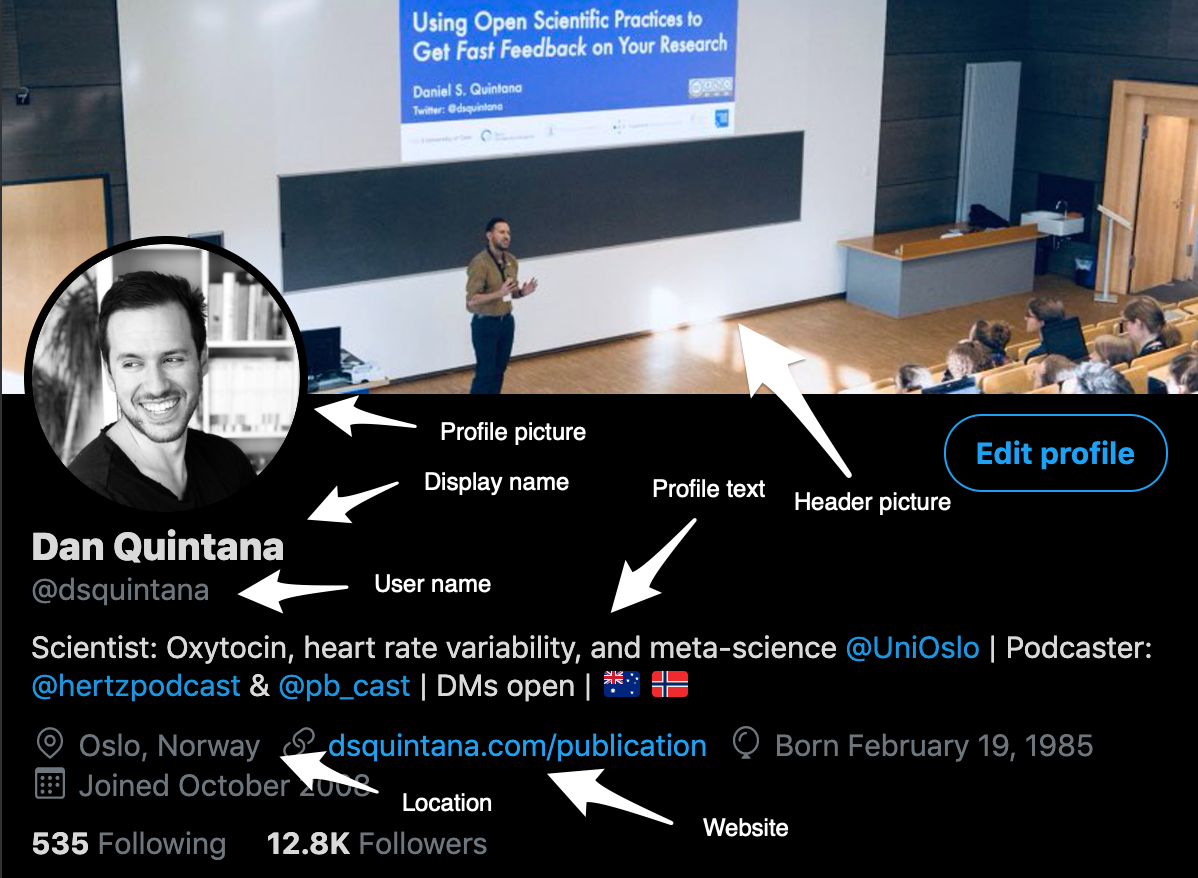
\includegraphics[width=0.8\linewidth]{images/profile} \hfill{}

\caption{The elements of a Twitter profile}\label{fig:unnamed-chunk-5}
\end{figure}

\hypertarget{your-profile-picture}{%
\subsection*{Your profile picture}\label{your-profile-picture}}
\addcontentsline{toc}{subsection}{Your profile picture}

It's important that you change your profile picture to something different from the default profile picture, as this helps reassure others that you're not a bot and also helps people identify you. The most obvious picture to use is one of yourself, but this isn't necessary. You can use an image of anything you want, really. In fact, some scholars have become quite well known for their unconventional profile images.

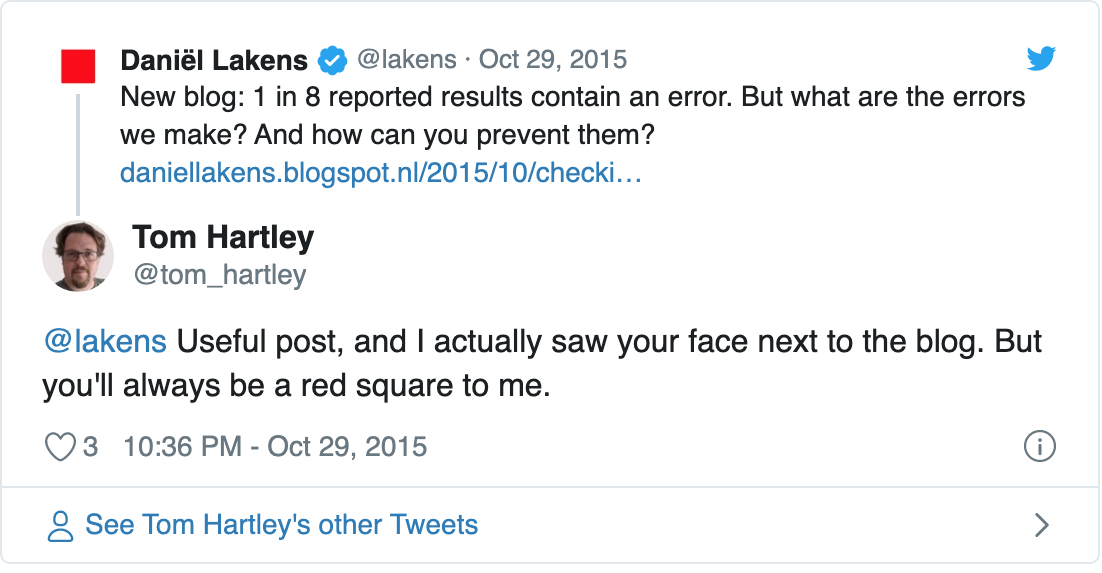
\includegraphics{twitter_book_files/figure-latex/tweet-about-red-square-1.png}

It's fine to change your image every now and then, but don't do this \emph{too} often as people may not easily recognize you when you tweet. Personally, I tend to identify tweets author via the profile image when scrolling through my Twitter feed, and I suspect others do the same.

You can use a JPEG or GIF file with a maximum size of 2MB. As Twitter is used on a range of devices with different screen sizes, Twitter recommends that profile photos are 400x400 pixels. But don't worry if your picture isn't exactly these dimensions.

\hypertarget{your-twitter-header-image}{%
\subsection{Your Twitter header image}\label{your-twitter-header-image}}

This is another opportunity for people to get a sense of what to expect when they follow you. If you would like some inspiration, get a free \href{https://canva.com/}{Canva} account and then search ``Twitter Header'' for some free design templates that use the required dimensions (1500 by 500 pixels).

Another common header image is a landscape shot of the region where you live (or where you grew up). Two other popular options are an image of you giving a presentation, or an image of your latest publication. There aren't any specific rules here, but use the opportunity to share your personality or to give a preview of the sort of things that you'll tweet. Twitter also has its own \href{https://www.flickr.com/photos/twitteroffice/sets/72157643560484885/}{header image gallery}, with images that have the recommended dimensions. You can also find some great images on \href{https://unsplash.com}{Unsplash}, which you can use with or without attribution.

\hypertarget{your-bio}{%
\subsection{Your bio}\label{your-bio}}

Share a short description of your research area and the sorts of thing that people can expect if they follow you. Bios are limited to 160 characters, which isn't a lot. You may also consider including the twitter handle of the institution you work at in your bio.

Feel free to add emoji to give your bio a little more personality. This can give you a few extra characters that you can use. For example, you can also use emoji to highlight your research area. If you are a neuroscientists, say, you could use a brain emoji).

\hypertarget{the-website-link}{%
\subsection{The website link}\label{the-website-link}}

This is another good opportunity for people to learn about you. As an academic, people will be interested to find out about your publications and your current projects. I think every research scientist should have their own website, as people \emph{will} Google you. You may miss out on opportunities, such as speaking invitations, if you don't have a website with your basic details. Many institutions provide staff and students with a profile page, but don't rely on this unless you have a permanent position. These institutional profile pages also tend to be quite inflexible regarding the kind of information that you can include.

If you have some familiarity with R, I've put together an \href{https://www.dsquintana.blog/free-website-in-r-easy/}{easy-to-follow guide} to make your own website for free. You can also use a Google Scholar profile, which you should set up if you haven't already.

\hypertarget{location}{%
\subsection{Location}\label{location}}

It's up to you for how specific you want to be when it comes to specifying your location. Adding your city could be helpful, as people may want to contact and meet you in person if they're traveling through your region. In theory, you don't have to put a single physical location in this field, with some people using this space to include two cities if they regularly commute between them or they want to include their hometown.

\hypertarget{the-anatomy-of-a-tweet}{%
\section*{The anatomy of a tweet}\label{the-anatomy-of-a-tweet}}
\addcontentsline{toc}{section}{The anatomy of a tweet}

Tweets can include text (up to 280 characters), 1-4 images (PNG or JPG), a single GIF, or a video. You can also post both text (including emoji) and one of the types of media described above.

\begin{figure}

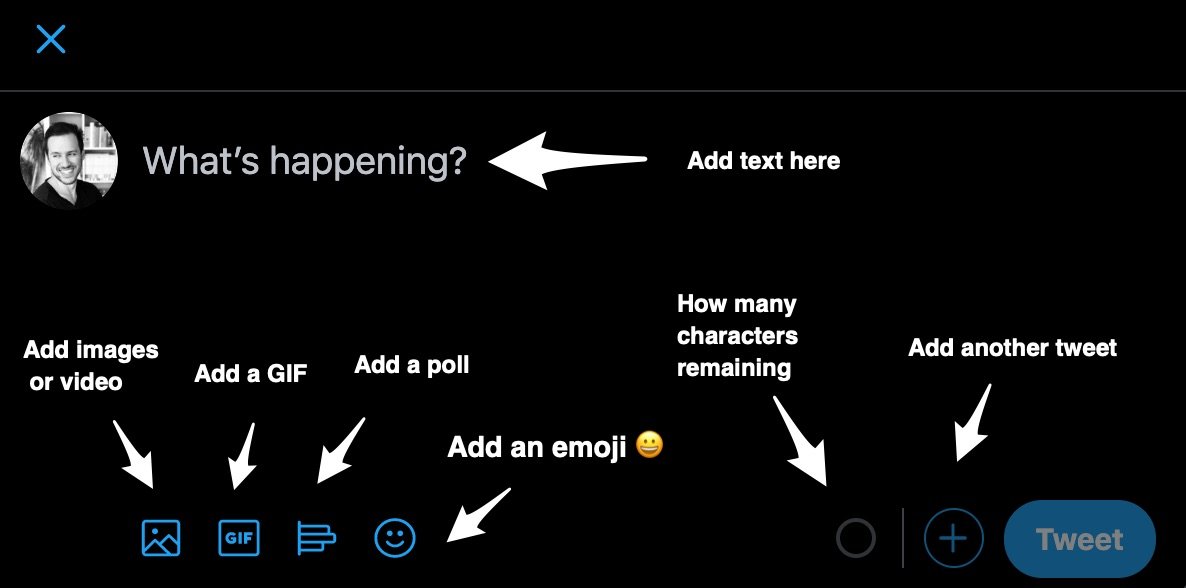
\includegraphics[width=0.8\linewidth]{images/compose} \hfill{}

\caption{The "compose" window.}\label{fig:unnamed-chunk-6}
\end{figure}

You can get pretty creative with emoji in your tweets.

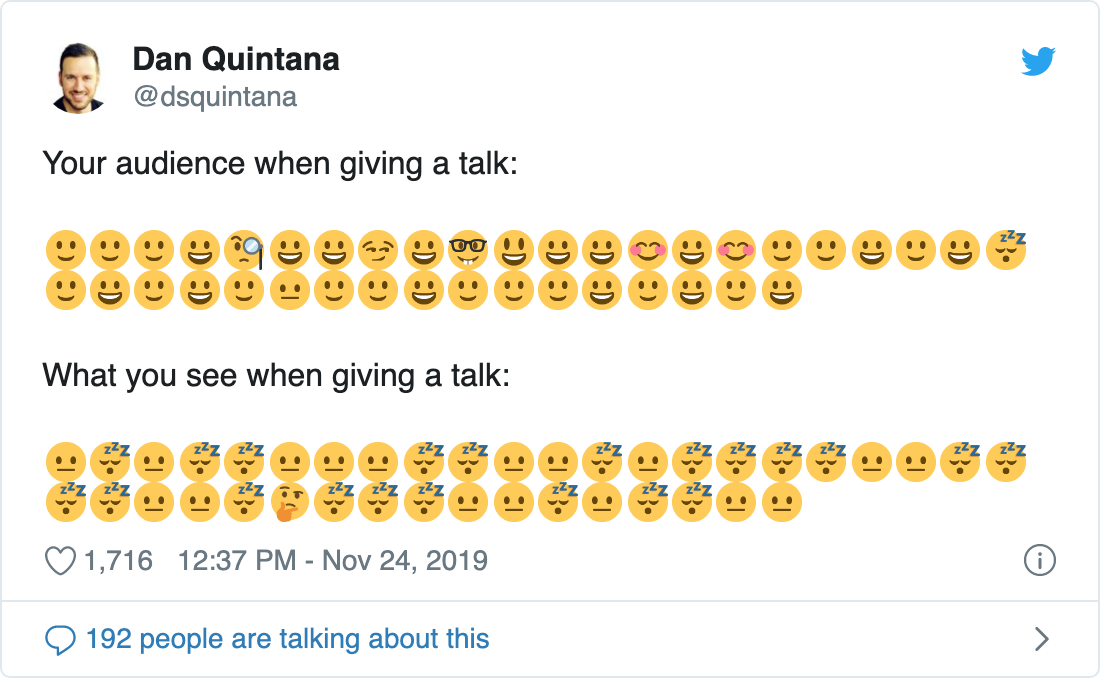
\includegraphics{twitter_book_files/figure-latex/tweet-about-emojis-1.png}

\hypertarget{using-text-in-your-tweets}{%
\subsection{Using text in your tweets}\label{using-text-in-your-tweets}}

Twitter was originally conceived as a SMS-based service, in which you could send text-only tweets via SMS.\footnote{Believe it or not, this SMS tweet-feature \href{https://help.twitter.com/en/using-twitter/twitter-sms}{still exists}.} The majority of tweets are text only, so this is Twitter's bread and butter.

Your text can also include website URLs. Regardless of the size of the URL, Twitter will treat each URL as 23 characters. You can also mention other Twitter users, by writing the `@' symbol, followed by their Twitter username, like this: @dsquintana. When you use the @ symbol and start typing a name, Twitter will try and guess which account you want to write via an autocomplete function. People that you already follow will be at the top of the list. When you mention other twitter users in your tweets, they will receive a notification (unless they have this option turned off).

\hypertarget{the-types-of-images-and-videos-you-can-include-with-your-tweets}{%
\subsection{The types of images and videos you can include with your tweets}\label{the-types-of-images-and-videos-you-can-include-with-your-tweets}}

In terms of static images, you can upload JPG and PNG files. Adding images are a nice way to help make your tweets stand out in people's timelines. Static images can be up to 5MB in size.

If you're looking for images to illustrate a tweet, I recommend doing a search on \href{https://unsplash.com/}{Unsplash}, as you can use these high-quality images without attribution (but you can attribute the photographer if you like). Here's an example of the kind of image you can find on Unsplash.

\begin{figure}

\includegraphics[width=0.8\linewidth]{images/unsplash} \hfill{}

\caption{I found this image on Unsplash by searching with the keyword "science"}\label{fig:unnamed-chunk-7}
\end{figure}

You can also upload GIFs, which are animated images, and search for GIFs directly by clicking on the ``GIF'' symbol when composing a tweet. GIFs have become a very popular way to share moving images. You can also use GIFs as a replacement for more conventional videos. If you're adding GIFs from another source, there's a 15MB limit when uploading from your desktop (5MB if uploading via the Twitter mobile app).

Additionally, you can also upload conventional videos via the Twitter website. Videos cannot be longer than 2 minutes and 20 seconds or larger than 512MB. There are a number of additional limitations when uploading videos via the Twitter website that you should also \href{https://help.twitter.com/en/using-twitter/twitter-videos}{be aware of}. Uploading videos via the Twitter mobile app is less restrictive in terms of file formats, as you can upload both MOV and MP4 files. If you have a video that's longer than two minutes and twenty seconds, you can upload the video to YouTube and then tweet the link to the video. I would also recommend posting a short preview of your YouTube video, as I demonstrate in the \protect\hyperlink{composing-tweets}{next chapter}.

\hypertarget{interacting-with-other-tweets}{%
\section*{Interacting with other tweets}\label{interacting-with-other-tweets}}
\addcontentsline{toc}{section}{Interacting with other tweets}

When you see other tweets in your main feed, you can primarily interact with them three ways: liking, retweeting, and replying.

\hypertarget{liking-tweets}{%
\subsection{Liking tweets}\label{liking-tweets}}

You can `like' a tweet by clicking on the little heart icon. This acknowledges both to the tweet author and to other people that you liked the tweet (e.g.~someone tweeted good news, an interesting article, or shared a funny meme). Liking can also be used as a token of support. For instance, if someone shares bad news, liking the tweet doesn't mean that you \emph{like} the news. Rather, liking the tweet is a show of support for the person who sent the tweet.

Just keep in mind that when you like a tweet, this \emph{might} appear in the feed of people that follow you, but probably won't. Also, others can quickly see which tweets you've liked via the ``Likes'' tab in your profile.

\begin{figure}

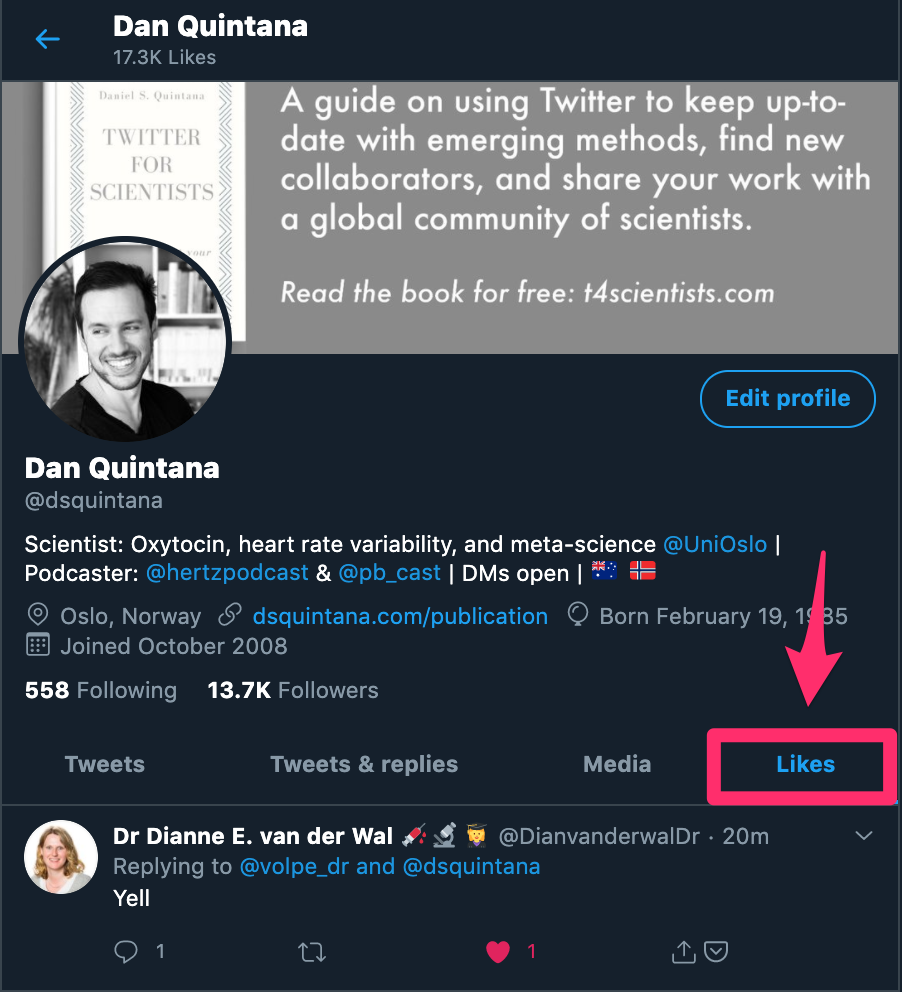
\includegraphics[width=0.8\linewidth]{images/likes} \hfill{}

\caption{The "Likes" column on your profile}\label{fig:unnamed-chunk-8}
\end{figure}

You might also see tweets that people you follow have liked in your feed too. Liking is also a useful way of acknowledging that you've read a tweet that mentioned you when you don't have the time to reply or the tweet doesn't warrant a reply for one reason or another. Remember, you don't \emph{have} to reply to someone who's mentioned you in a tweet, but it's good courtesy to do so\footnote{Of course, this doesn't apply to harmful tweets. In section 5.3 I discuss how to block, mute, and report harmful tweets}.

\hypertarget{retweeting}{%
\subsection{Retweeting}\label{retweeting}}

If you come across a tweet that you think your followers would value, then you can use the Retweet function. When you click on the Retweet button, you'll get two options. The first option is a conventional retweet, which will appear in your follower's timeline, as if one of the users they follow tweeted it. Below is an example of a retweet. Your followers will see that you've retweeted someone else's tweet, like this.

\begin{figure}

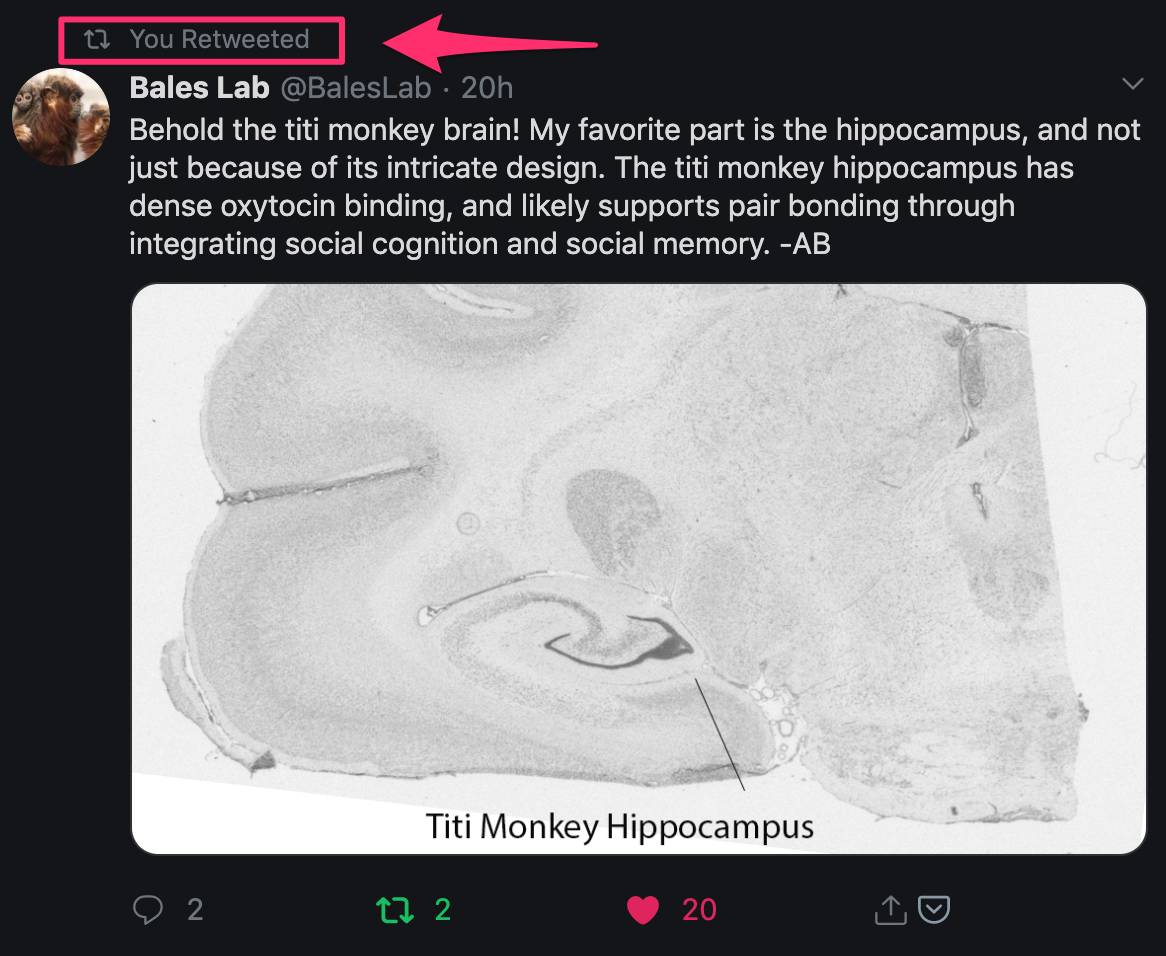
\includegraphics[width=0.8\linewidth]{images/retweet} \hfill{}

\caption{A retweet example}\label{fig:unnamed-chunk-9}
\end{figure}

The second option is to ``Retweet with comment''. This allows you to share the tweet, along with your comment above. This is a good way to describe \emph{why} you're retweeting a particular tweet.

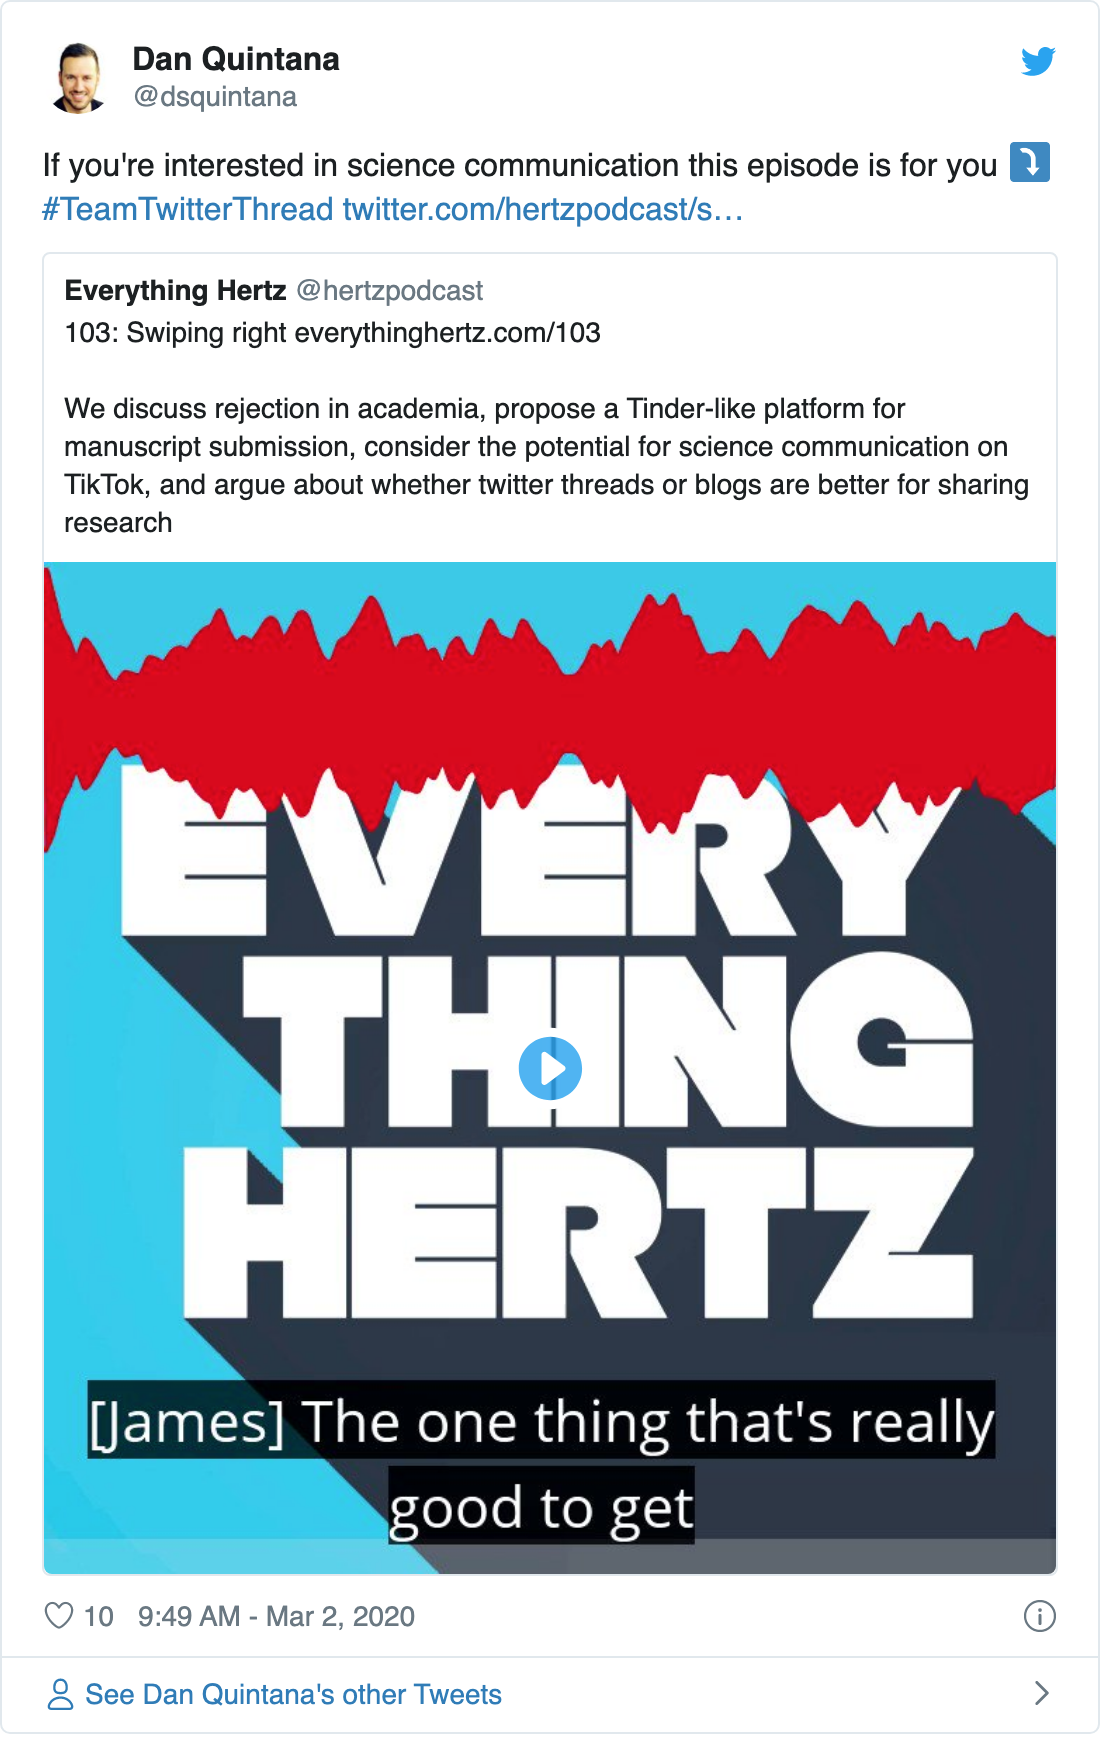
\includegraphics{twitter_book_files/figure-latex/tweet-about-quote-RTs-1.png}

Here's another example of a retweet with a comment.

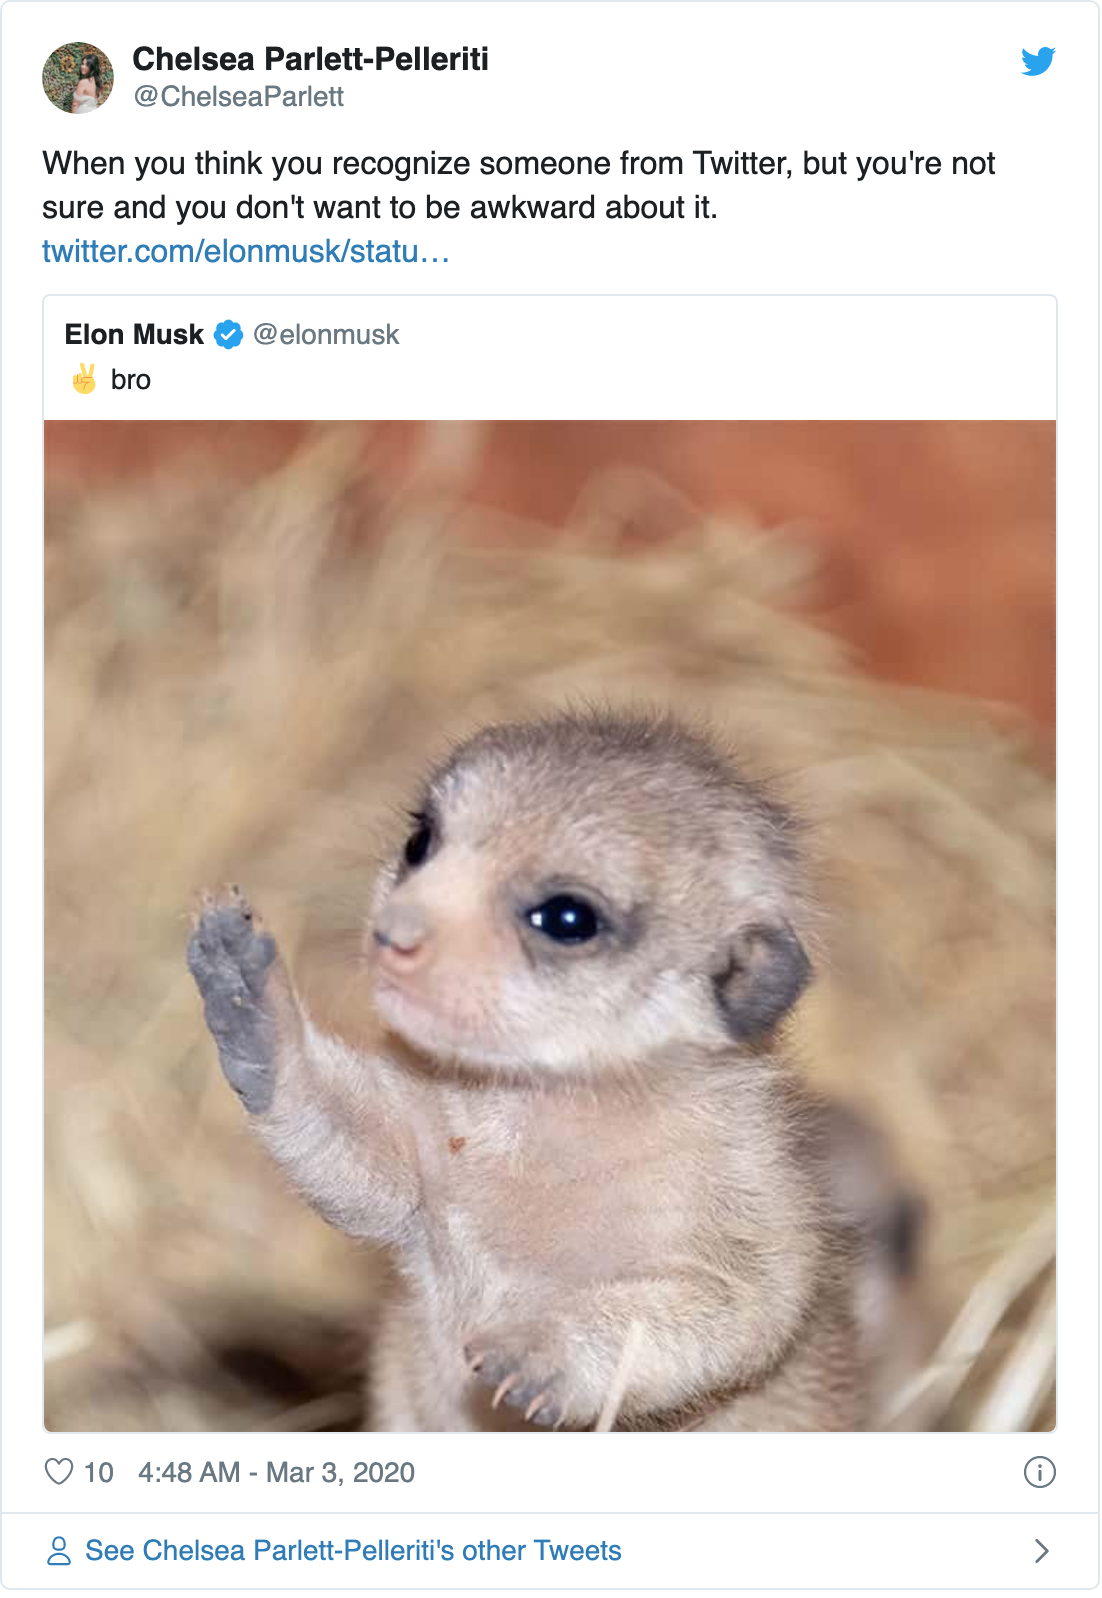
\includegraphics{twitter_book_files/figure-latex/tweet-about-quote-RTs-example2-1.png}

Remember, if you want your followers to see a tweet in your timeline (e.g., a colleague announces a new paper), then you'll need to retweet it---only ``liking'' the tweet isn't enough.

\hypertarget{replying-to-tweets}{%
\subsection{Replying to tweets}\label{replying-to-tweets}}

One of the great things about Twitter is that it makes it much easier to chat with people that are otherwise difficult to contact via email. An email (usually) includes a salutation, some brief chit-chat, the actual question or comment, then a sign off. With twitter you just write the question or comment. In the following example, I'm replying to a tweet from \href{https://twitter.com/xieyihui}{@xieyihui}, who quote-retweeted one of my tweets.

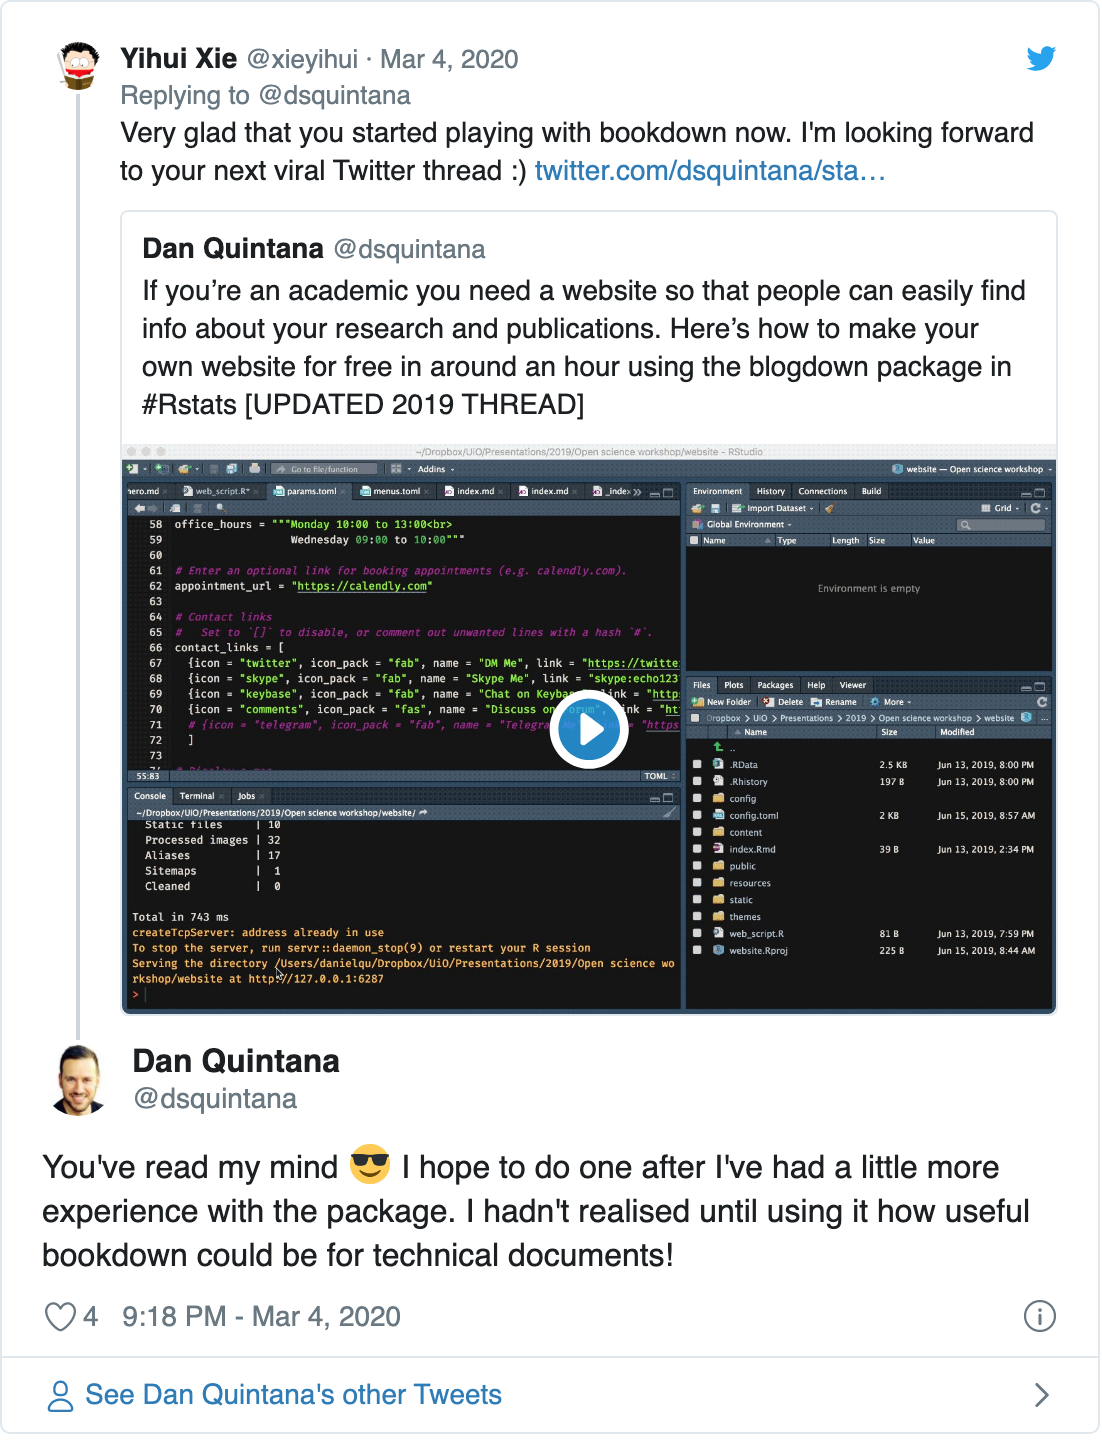
\includegraphics{twitter_book_files/figure-latex/tweet-about-reply-1.png}

Replying to tweets is one of the best ways to build your network, as it helps you to establish your expertise in your topic area. All the usual tweeting options are also available for replies.

\hypertarget{direct-messages}{%
\section*{Direct messages}\label{direct-messages}}
\addcontentsline{toc}{section}{Direct messages}

You can send a private direct message (often abbreviated as a ``DM'') to other Twitter users. This is a useful feature if you want to ask a question, but would rather the question wasn't public. But keep in mind that you can only send direct messages to people that are following you or people that have \href{https://help.twitter.com/en/using-twitter/direct-messages\#receive}{opted in to recieve direct message from anyone}. I've decided to keep my direct messages open, so that anyone can contact me, but this is up to you. In addition, you can send group direct messages if you would like to privately chat in a group.

If you want to get in contact with another scholar who's active on Twitter, a direct message is generally more effective than an email as there's much less friction writing a direct message. There's no need for long-winded formalities, formatting, or long email signatures. Just keep your message short if you're contacting someone you don't know for the first time. If your message doesn't fit on a smartphone screen, it's far too long.

\hypertarget{your-twitter-style}{%
\section*{Your Twitter style}\label{your-twitter-style}}
\addcontentsline{toc}{section}{Your Twitter style}

\hypertarget{how-personal-should-you-tweets-be}{%
\subsection{How Personal should you tweets be?}\label{how-personal-should-you-tweets-be}}

This is up to you, so share whatever you're comfortable with. Some people like to keep their personal and academic lives separate, and others like to mix things up. One benefit of sharing some personal tweets is that it gives your Twitter account a little more personality, but don't feel that you \emph{have} to do this.

\hypertarget{finding-your-twitter-voice}{%
\subsection{Finding your twitter ``voice''}\label{finding-your-twitter-voice}}

Be yourself. Trying to be someone you're not on Twitter is not sustainable in the long run. Another aspect to consider is how ``professional'' you want your Twitter account to be. Some people think that you shouldn't tweet anything you wouldn't say in front of a live audience of your peers. I understand this sentiment, and realize that different fields have different conventions. But at the same time, you also need to think about the \emph{context} of Twitter, which is typically more casual than doing an academic talk. Just keep in mind that anyone can search through your tweets, if they want. Finally, some institutions have a social media policy, so it's best to check if your institution has one before you start tweeting.

\hypertarget{using-a-pseudonym}{%
\subsection{Using a pseudonym}\label{using-a-pseudonym}}

Some scientists would prefer to not use their real identities on Twitter, for various reasons, and that's ok! While not using a real identity can limit \emph{some} of the perks of Twitter (e.g., research collaborations), a pseudonymous user can still reap several benefits. But don't take it from me, here's \href{https://twitter.com/PsyBrief}{@PsyBrief}, who used to have a pseudonymous account (but since identified himself), on what he had gotten out of Twitter while he was pseudonymous.


\includegraphics{twitter_book_files/figure-latex/tweet-about-pseudonym-1.png}

\hypertarget{finding-people-to-follow}{%
\section*{Finding people to follow}\label{finding-people-to-follow}}
\addcontentsline{toc}{section}{Finding people to follow}

There are various ways to find people to follow on Twitter. Try searching for some key words of interest in \href{https://help.twitter.com/en/using-twitter/twitter-search}{Twitter search}, and have a look at the users behind these tweets. If you've found a few interesting accounts, have a look at who \emph{they're} following. Over time, you'll find more accounts as you'll come across more retweets from accounts that you don't follow already.

If you click on the ``People'' tab when searching (see image below) this will show you accounts that have a specific keyword in their bio.

\begin{figure}

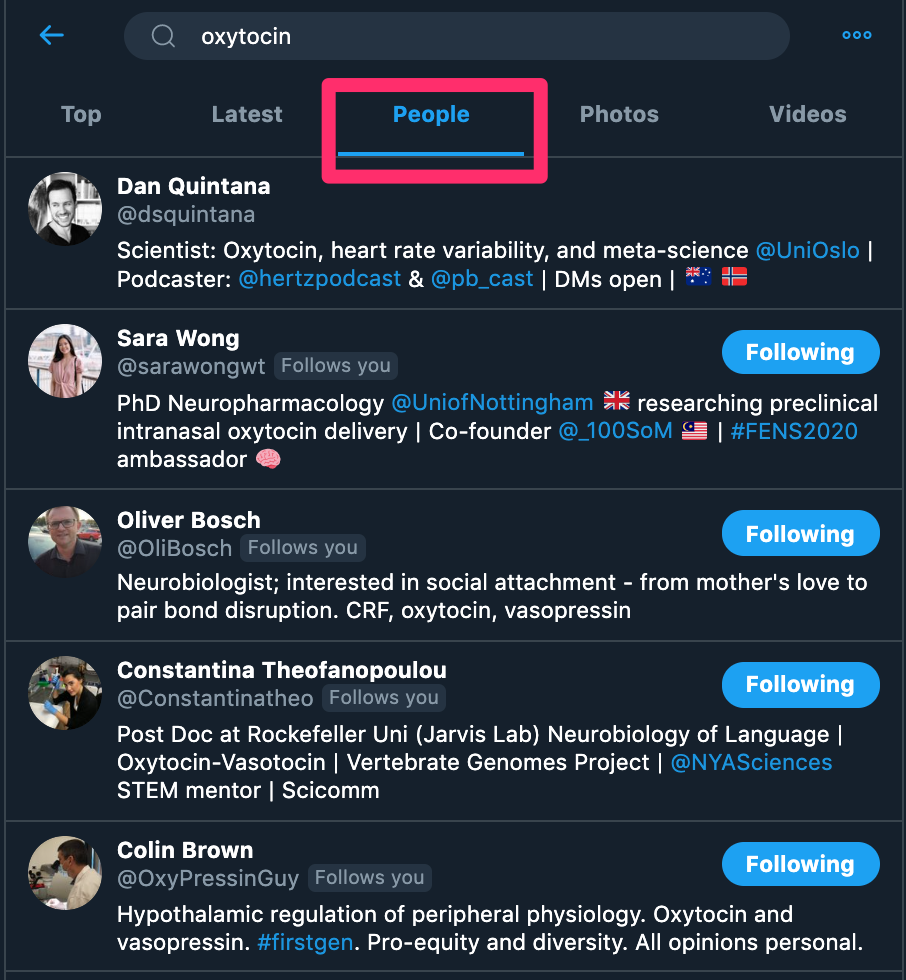
\includegraphics[width=0.8\linewidth]{images/bio_search} \hfill{}

\caption{Searching for keywords in bios}\label{fig:unnamed-chunk-10}
\end{figure}

You will also see a ``Who to follow'' box next to your main feed on the desktop site. These are \emph{usually} good recommendations, but sometimes you get some odd suggestions. Either way, these recommended users are worth checking out from time to time. These recommendations are based on the accounts the people you are following are interacting with and following themselves.

If your bio and recent tweets align with the interests of the people you follow, they may follow you back. However, people aren't obligated to follow you back so don't expect this as a given.

Remember, you can always \href{https://help.twitter.com/en/using-twitter/how-to-unfollow-on-twitter}{``unfollow''} people. Twitter \textbf{will not} send people a notification if you unfollow them. Alternatively, you can also \href{https://help.twitter.com/en/using-twitter/twitter-mute}{``mute''} people. This means that you're still following them, but their tweets won't appear in your feed.

\hypertarget{composing}{%
\chapter{Composing tweets}\label{composing}}

The most common question I get at social media workshops that I've run is, ``What should I tweet?''. There is no easy answer to this, because every researcher and their subfield is different. But regardless of your subfield, \textbf{the best way to engage your followers is to either entertain or educate}. In other words, you should aim to help people either pass time or save time. Being entertaining doesn't come naturally to most people, so don't worry if this isn't you. But as a scientist, you are very well-placed to educate, no matter your level of training.

Thanks to \protect\hyperlink{beginner}{Chapter 1}, you're up to speed with the general mechanics of Twitter. You also just learned about the ``entertain or educate'' principle, with \emph{any} scientist ready to educate. But even when arriving at this point, many scientists hit a wall, because they believe they can only tweet the finished product of their work, which is typically papers. But as soon as you realise that the \emph{process} of your work is just as interesting as the \emph{output}, then things become much easier. You're going to see a few examples of this below.

When it comes to tweet frequency, it's hard to give any firm recommendations. Whether you're tweeting too much depends on how many people your followers are following, and how much \emph{they} tweet. So, this means that the ``too much'' threshold is different for everyone. In my opinion, I think it's fairly difficult to tweet too much. In the early days of Twitter (or any social network), where users didn't follow that many people, it was pretty easy to flood someone's timeline. But now, people tend to follow hundreds (sometimes thousands) of accounts, so this is harder to do. I think the upside of more tweets outweighs the downside a few people unfollowing you because they think you tweet too much. You never know which tweets other people will find interesting.

\hypertarget{some-example-tweets}{%
\section*{Some example tweets}\label{some-example-tweets}}
\addcontentsline{toc}{section}{Some example tweets}

\hypertarget{tweeting-about-your-own-research-papers}{%
\subsection{Tweeting about your own research papers}\label{tweeting-about-your-own-research-papers}}

This is one of the most common tweets you'll see from scientists who aren't very active on Twitter. When a new paper is published, they'll log on, post the title of their paper with a link to the paper, and then log off until their next paper is published. There are so many more types of tweets that you can compose, but I'm going to walk through how you can lift your game with these types of tweets, which are one of the main reasons many scientists are on Twitter.

\textbf{1. Add an image from the paper to go with the tweet.} Have a look through the paper to see if there's a striking image that can be used. If there are no figures in your paper, you can just take a screenshot of the abstract or a particularly interesting part of the paper. \href{https://evernote.com/products/skitch}{Skitch} is a handy app for screenshots, as you can easily annotate and highlight images. If you're on your smartphone, you can also just take a screenshot and crop the image to your needs. You can add up to four images per tweet, so if you have more than one striking image you can take advantage of this

\textbf{2. Add a quote from the paper.} Find a striking quote from the paper to include in your tweet. You can either write this as text, or take a screenshot of it and then highlight the quote, using Skitch or other software.

\textbf{3. Tag your co-authors and the journal.} Co-authored papers are a team effort, so you should acknowledge your team. In addition, this gives your followers the chance to find more people to follow. If you have a lot of co-authors, remember that you can also tag authors in images as well. This means that your co-authors will get notified of the tweet and others can see who else is involved in the resesarch.

\textbf{4. Add your own commentary of the paper.} If you're not including a quote, you should share \emph{why} you think the paper is interesting. Maybe it's your first paper or it's part of a project you've been working on for a long time.

\textbf{5. Add a link to a non-paywalled version of the paper.} People might see the tweet, but not bother clicking on the link if they do not have institutional access to the journal. However, if you include a link to a preprint or a postprint\footnote{A preprint is a version of an article that is posted to a preprint repository before peer-review. Most journals allow you to submit papers that have been posted as preprints and do not consider this dual-publication. Check your journal's policies. A postprint is a version of paper that has undergone peer-review but has not been typeset. These are typically posted to the author's personal or institutional website. Postprints are usually just a PDF version of the final Word document that was sent to the journal. Unlike preprints, journal policies vary regarding postprints, so it's best to check before uploading one.}, then people know they can easily access the paper.

In the following example of a paper I co-authored, I mention a summary of the results, highlight the sample size as this is a notable feature of the paper, tag my co-authors who are on Twitter, include a link to a postprint of the article, and attach a figure from the article.


\includegraphics{twitter_book_files/figure-latex/tweet-about-paper-1.png}

Here's another good example, with \href{https://twitter.com/GuyProchilo}{@GuyProchilo} sharing his first first-author paper. Notice that Guy tags his co-authors, the journal, adds a hashtag (\#IOpsych) relevant to his research field in this tweet (Industrial-organisational psychology), and includes a striking image of the paper.

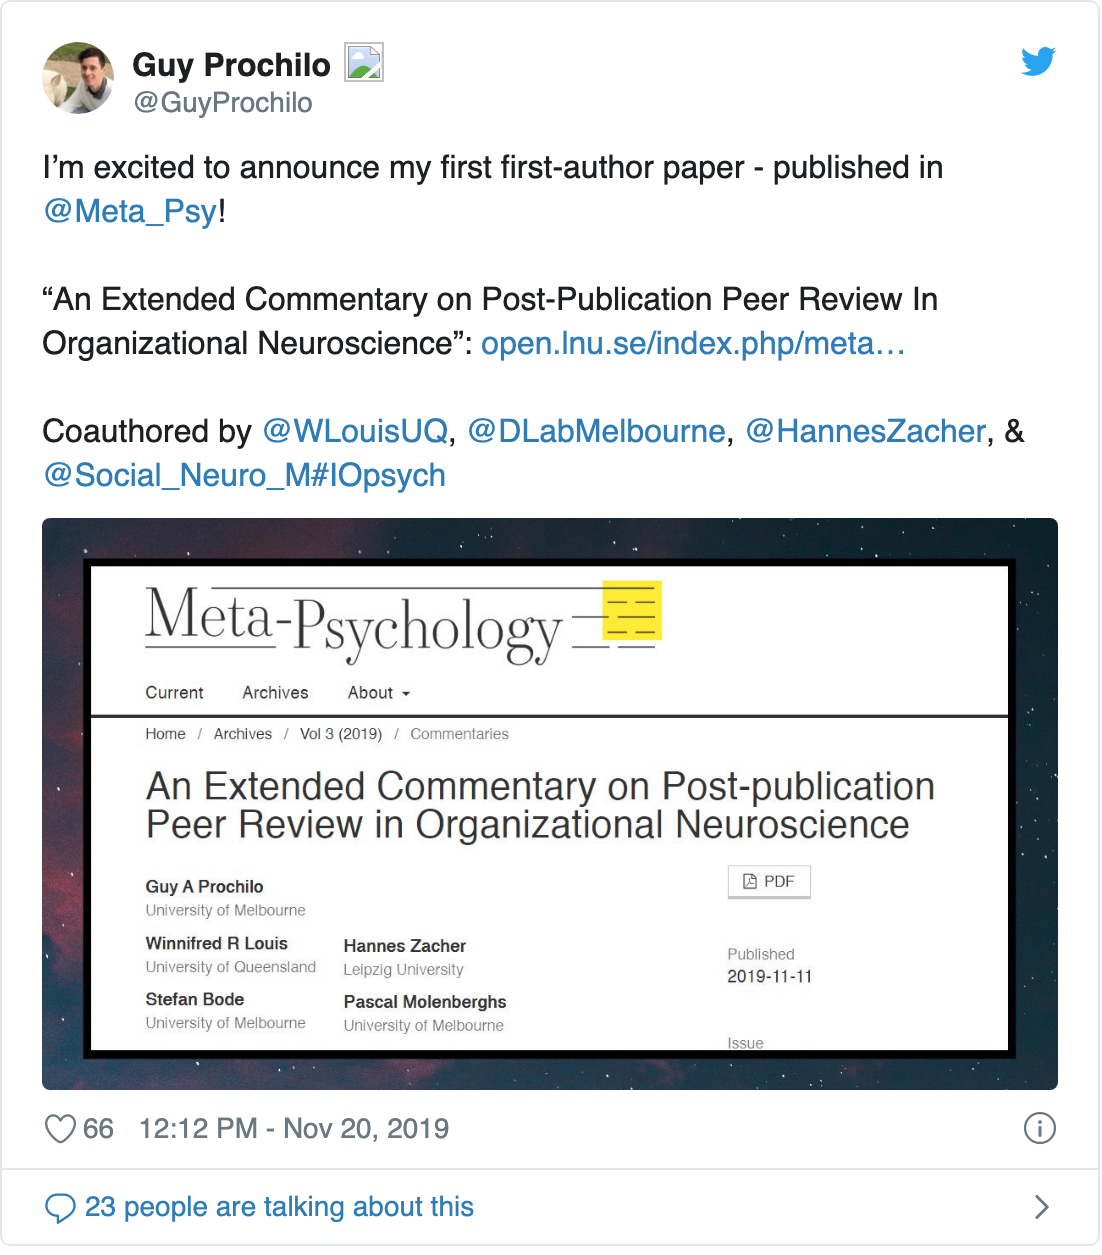
\includegraphics{twitter_book_files/figure-latex/tweet-from-guy-1.png}

While single tweets announcing new papers can be an effective way to share your new work, I think a thread, which are a series of connected tweets, does a better job---see \protect\hyperlink{advanced-twitter-skills}{Chapter 4} for how to make an effective thread to introduce your new work.

\hypertarget{tweeting-about-other-peoples-research-papers}{%
\subsection{Tweeting about other people's research papers}\label{tweeting-about-other-peoples-research-papers}}

There are only so many articles that you can co-author. So in addition, you should also share papers that you find interesting. If you haven't already, you should set up new publication alerts using keywords that are relevant to your work. Pubmed and Google Scholar are popular options for setting up paper alerts. The advantage of Google Scholar is that it will also capture new preprints and theses.

Below is an example of tweeting a link to a new paper, in which I added an image and quote from the paper, and mentioned the lead author and the journal that it was published in.

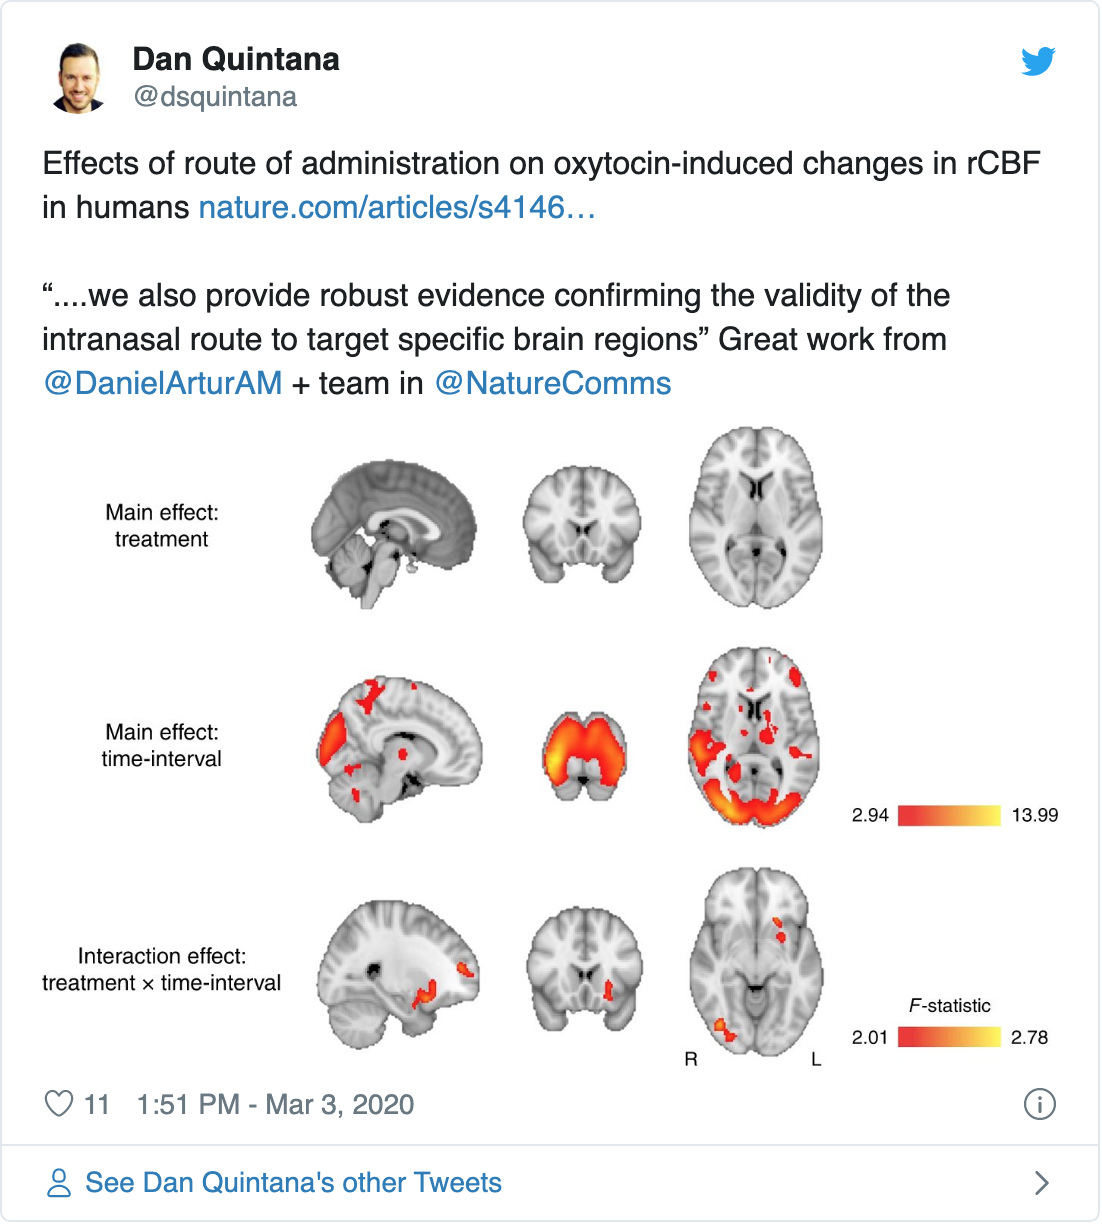
\includegraphics{twitter_book_files/figure-latex/tweet-about-paper-with-image-1.png}

\hypertarget{sharing-information-about-yourself}{%
\subsection{Sharing information about yourself}\label{sharing-information-about-yourself}}

Twitter provides a great way to connect with other researchers and to share information about yourself that you typically can't convey in a scientific paper. This is the sort of information that you could only normally learn in person, such as at a conference or a lab visit. But as travel is expensive and time-consuming, this option isn't open for everyone.

Here's an example from \href{https://twitter.com/_DaniBeck}{@\_DaniBeck}.

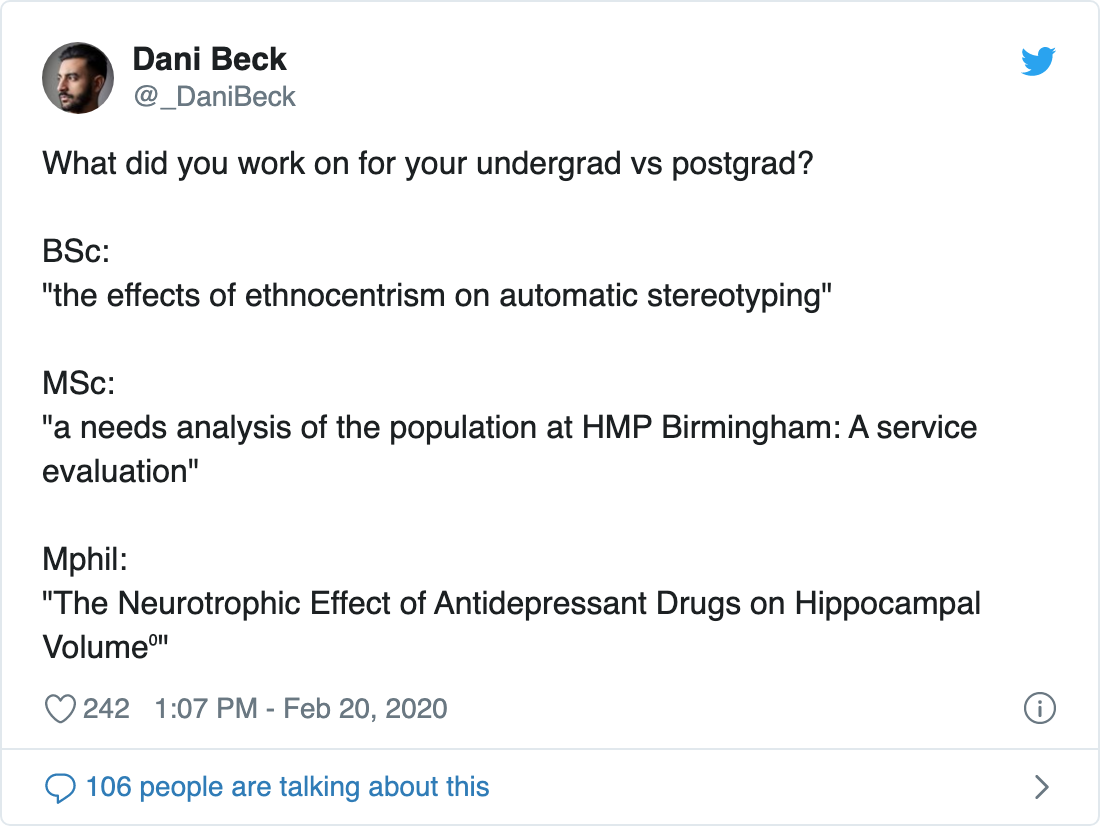
\includegraphics{twitter_book_files/figure-latex/tweet-introduction-1.png}

\hypertarget{sharing-your-toolkit}{%
\subsection{Sharing your toolkit}\label{sharing-your-toolkit}}

As scientists, we use several tools in our day-to-day work. Even if these tools seem commonplace to you, your followers will appreciate learning about new ways to do their work. Here's an example of me tweeting about the \href{https://bookdown.org/home/}{`bookdown' R package}, which I've used to write this book.


\includegraphics{twitter_book_files/figure-latex/tweet-toolkit-1.png}

Notice that the link has been converted into a small image with information, which is called a \href{https://developer.twitter.com/en/docs/tweets/optimize-with-cards/overview/abouts-cards}{Twitter Card}. This is a feature of some websites (including this one), which include Twitter Card information in their underlying code. If you're tweeting from your smartphone, the Twitter Card will appear (if it's available) as soon as you enter the link. This doesn't occur when tweeting from your desktop, but you can quickly check if there's a Twitter Card associated with the link you're going to post on the \href{https://cards-dev.twitter.com/validator}{Twitter Card Validator} website. If the Twitter Card contains a nice image then you might not need to add your own. You can also delete the Twitter Card from your tweet as well.

\hypertarget{asking-a-question}{%
\subsection{Asking a question}\label{asking-a-question}}

Twitter can be a great way to get advice. If you don't have many followers, you should also consider tagging experts that might know the answer (but don't spam people, so use this sparingly). Here's an example that I used, which was also used for researching this book.

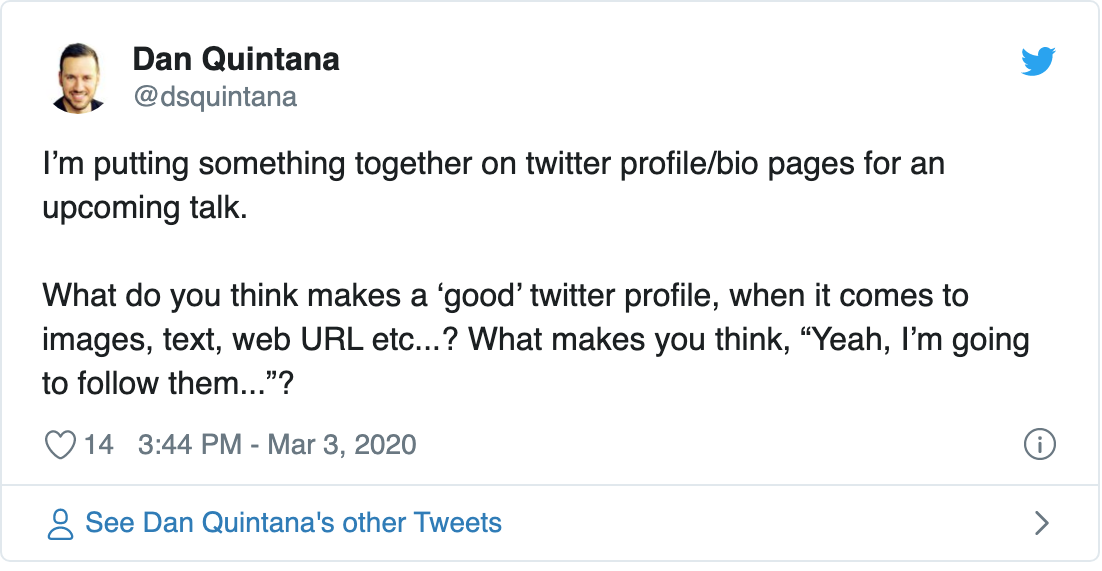
\includegraphics{twitter_book_files/figure-latex/tweet-ask-question-1.png}

This book is written for both HTML (online) and PDF (print) output. This is a book about Twitter, so I use a lot of tweet examples. One benefit of an online version is that you can embed tweets, which means that readers can visit the tweet's original source and read any replies to the tweet. It's also easy to see at a glance how many people have engaged with the tweet, as these numbers are attached to the bottom of embedded tweets. However, converting a HTML element into a image for a PDF is not as straightforward as you would think, as you essentially have to take a screenshot for each the tweet. To avoid this extra work, I put a call out on Twitter:

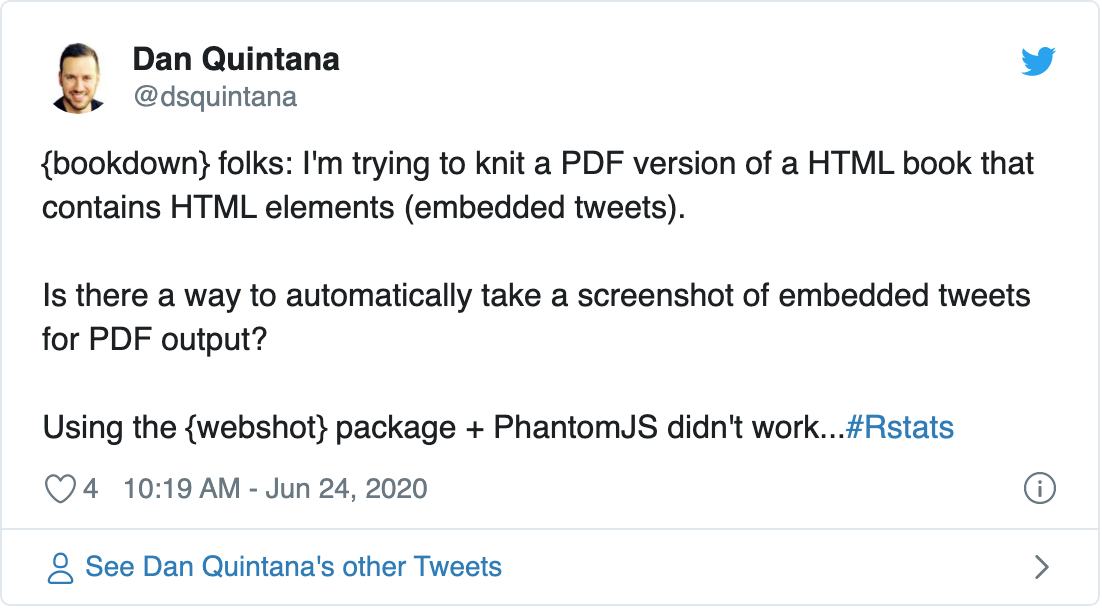
\includegraphics{twitter_book_files/figure-latex/tweet-call-out-1.png}

Fortunately, Garrick Aden-Buie (\href{https://twitter.com/grrrck}{@grrrck}) found this tweet and updated his \href{https://github.com/gadenbuie/tweetrmd}{`tweetmd' R package}, which solved my problem.

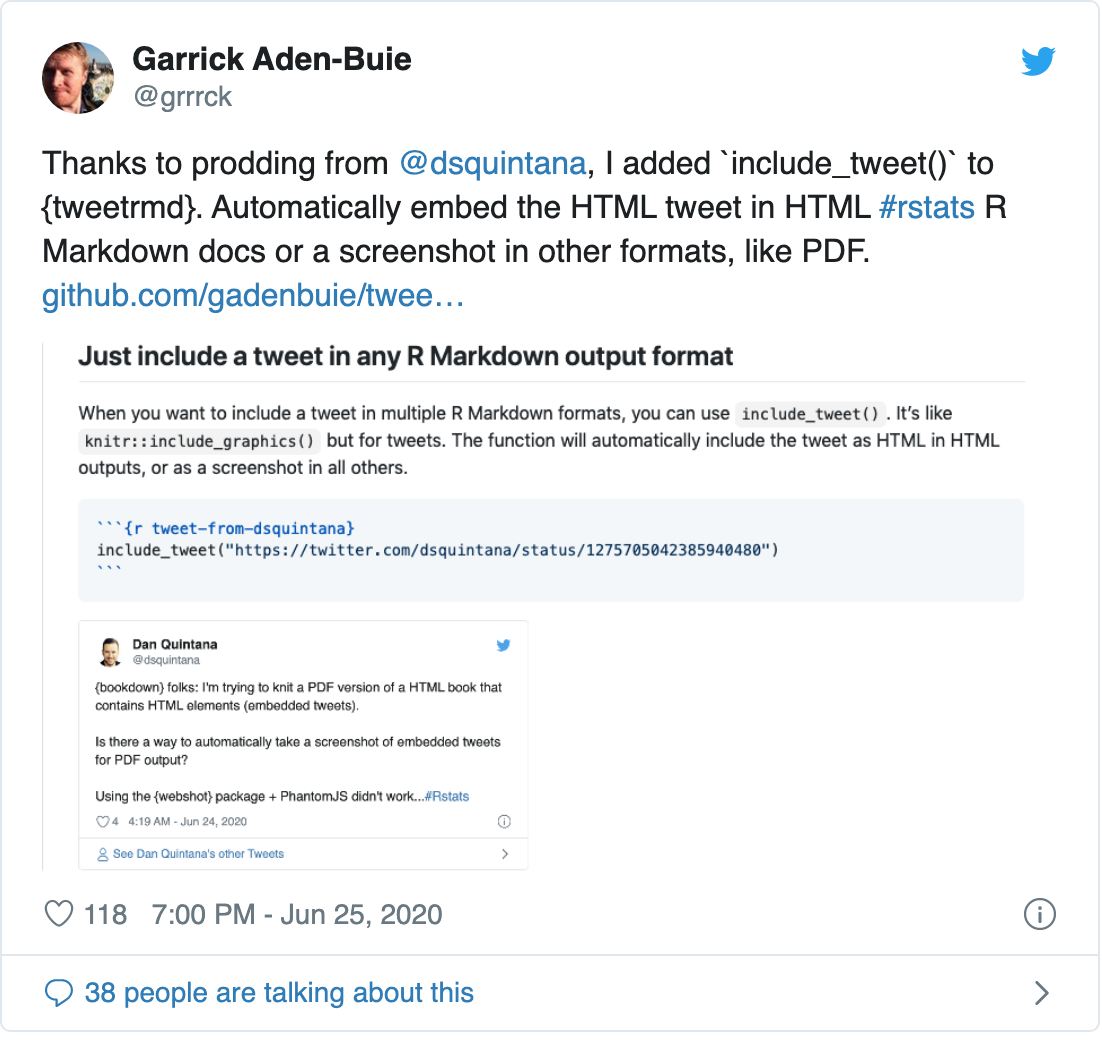
\includegraphics{twitter_book_files/figure-latex/tweet-tweetmd-1.png}

\hypertarget{answering-questions}{%
\subsection{Answering questions}\label{answering-questions}}

A great thing to tweet when you have have nothing to tweet is to help other people by answering their questions. There are several hashtags that are often used by scientists to ask questions, such as \#AcademicChat and \#PhDchat. What might seem like an easy solution to you may save someone else hours of work.

\hypertarget{replying-to-tweets}{%
\subsection{Replying to tweets}\label{replying-to-tweets}}

One of the fastest ways you can build connections on Twitter and to establish yourself as an expert in your area is to reply to other people's tweets. This seems counterintuitive, as one would think that conventional tweets are a better way to achieve these goals, but replies are almost guaranteed to be seen by the person you're replying to, whereas conventional tweets may not be seen at all (or quickly scrolled past), especially if you're new to Twitter. If others are following both yourself and the person you're replying to, they'll see the original tweet and your reply in their feed.

\hypertarget{sharing-memes}{%
\subsection{Sharing memes}\label{sharing-memes}}

Memes are a fun and effective way to demonstrate knowledge and authority in your research area. Notice in this example that this tweet was a quote retweet, so that people can see that I've remixed someone else's tweet.

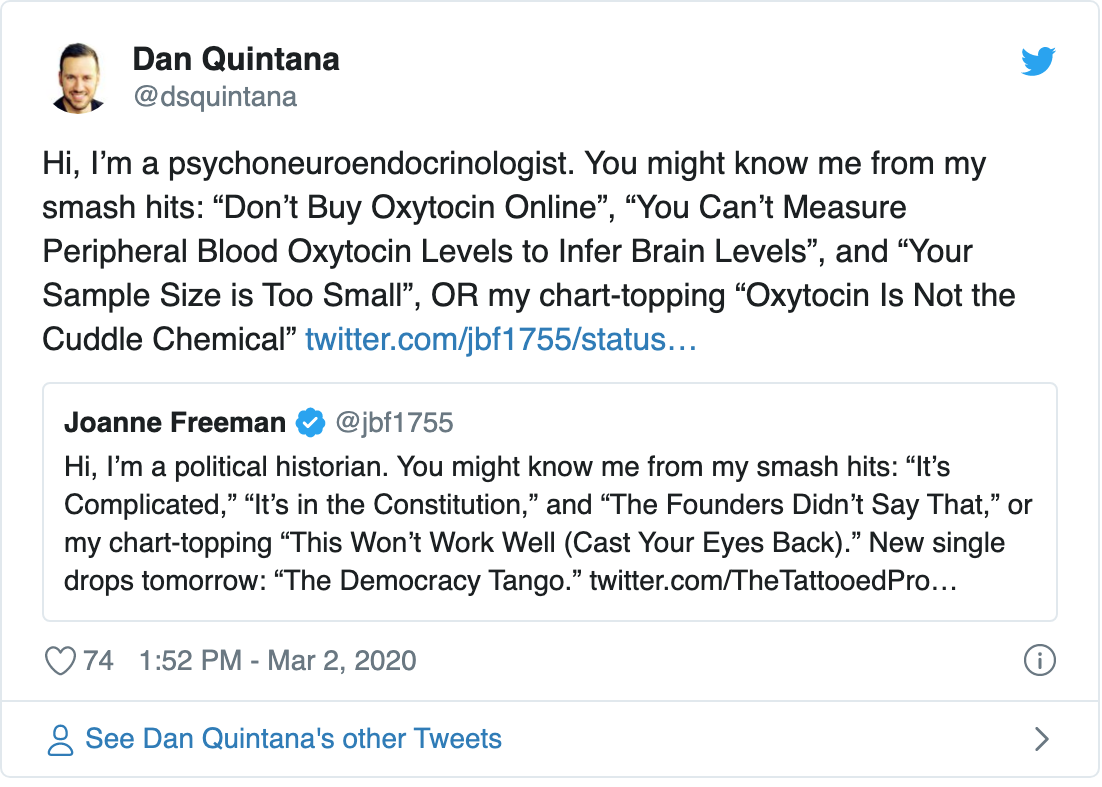
\includegraphics{twitter_book_files/figure-latex/tweet-meme-1.png}

\hypertarget{sharing-videos}{%
\subsection{Sharing videos}\label{sharing-videos}}

You can include a video that's up to two minutes and twenty seconds long in your tweets. In the following tweet, I've included a link to an eleven-minute instructional YouTube video. I can't show the entire video due to Twitter's limits, so I've included a short preview to entice people to click on the link to the full video.

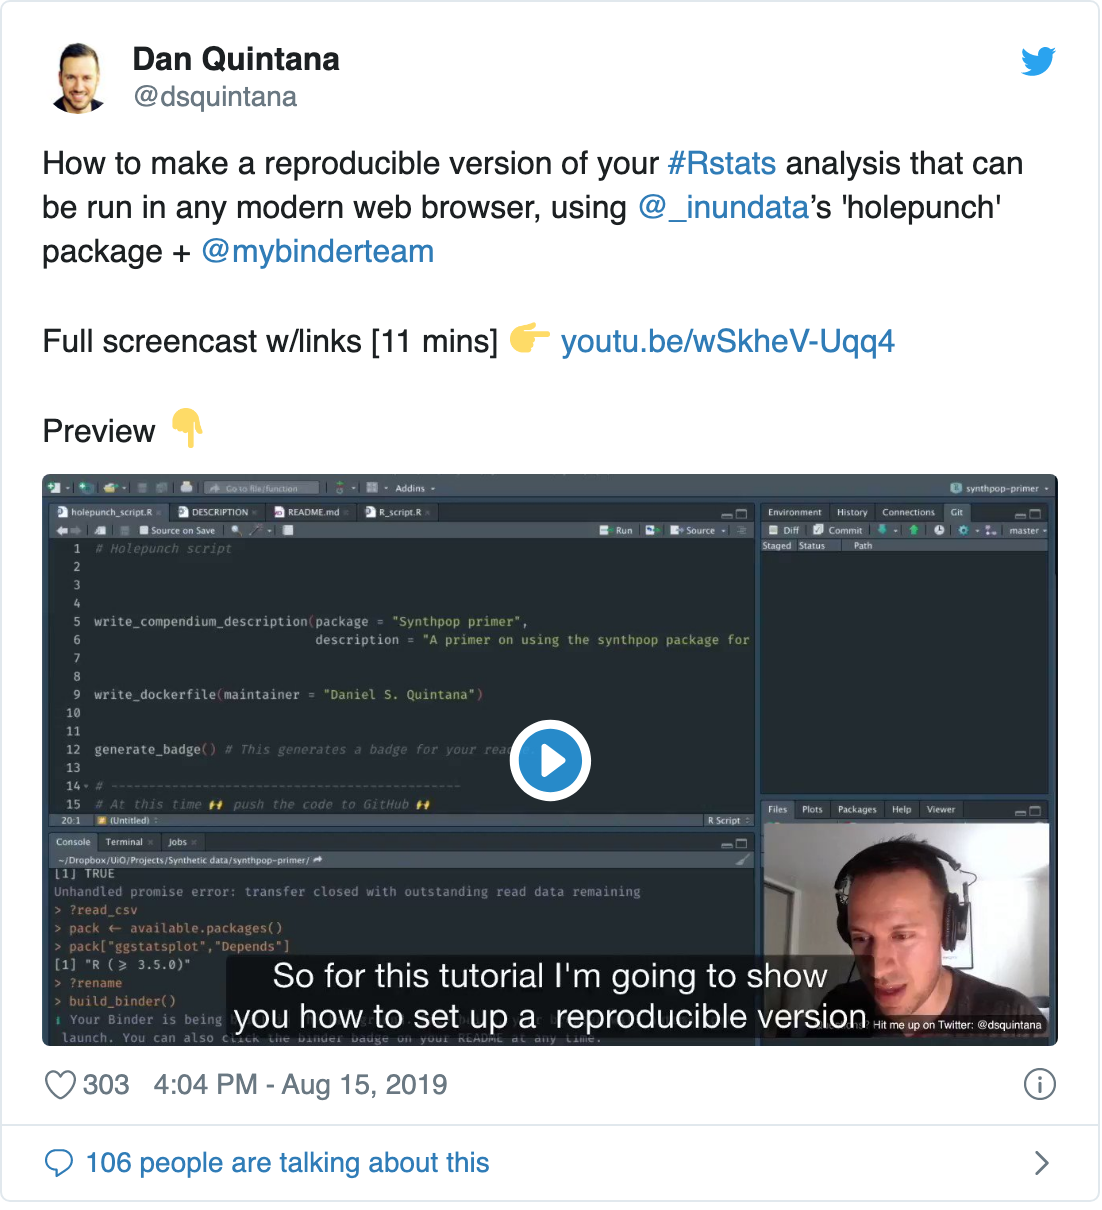
\includegraphics{twitter_book_files/figure-latex/tweet-video-1.png}

If I was only to post a link to the video on YouTube, the Twitter Card would only show a static image. This is better than nothing, but you're much better off with a short preview.

Also note that in this tweet I used the \#Rstats hashtag, I tagged the author of the R package and tagged the software service I used.

People can't always listen to audio when they're scrolling Twitter, so it's a good idea to include subtitles. This also increases accessibility for those with hearing impairments. When you upload your video to YouTube, it can \href{https://support.google.com/youtube/answer/6373554}{automatically transcribe your audio}. In my experience, the transcription is about 80\% accurate, so you will need to do \emph{some} editing of the transcription. However, this is much quicker than transcribing your video or audio clip from scratch. Another option for adding subtitles to your video is the \href{https://www.apalon.com/clipomatic.html}{``Cliptomatic'' app}. Like YouTube, the transcription is about 80\% accurate, but the editing function is pretty easy to use

\hypertarget{document-your-experiences}{%
\section*{Document your experiences}\label{document-your-experiences}}
\addcontentsline{toc}{section}{Document your experiences}

I hardly ever sit down and think, ``what will I tweet?''. Most of my tweets are simply offcuts of work I'm already doing, or things I'm already discussing in real life with colleagues.

For example, I was recently having a chat with some colleagues about grant applications. I told them a principle I used to write my applications, which they found useful. So I turned this into a tweet, which also seemed to resonate on Twitter.

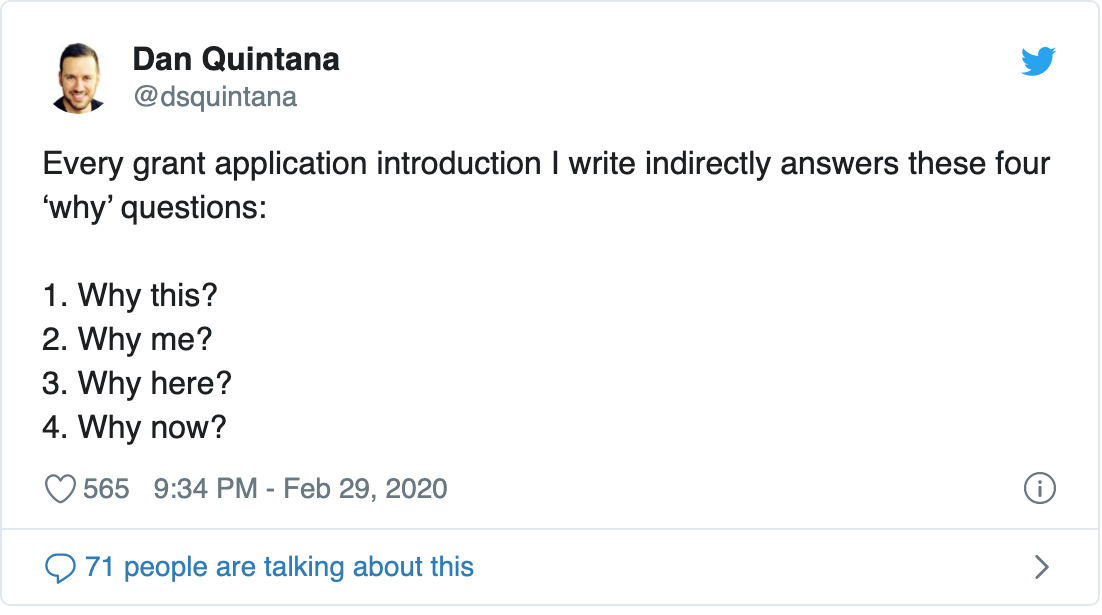
\includegraphics{twitter_book_files/figure-latex/tweet-grant-1.png}

This thread is another example of \href{https://austinkleon.com/show-your-work/}{``showing my work''}. I didn't have to think of something new to tweet, as I essentially copy and pasted my reply email.

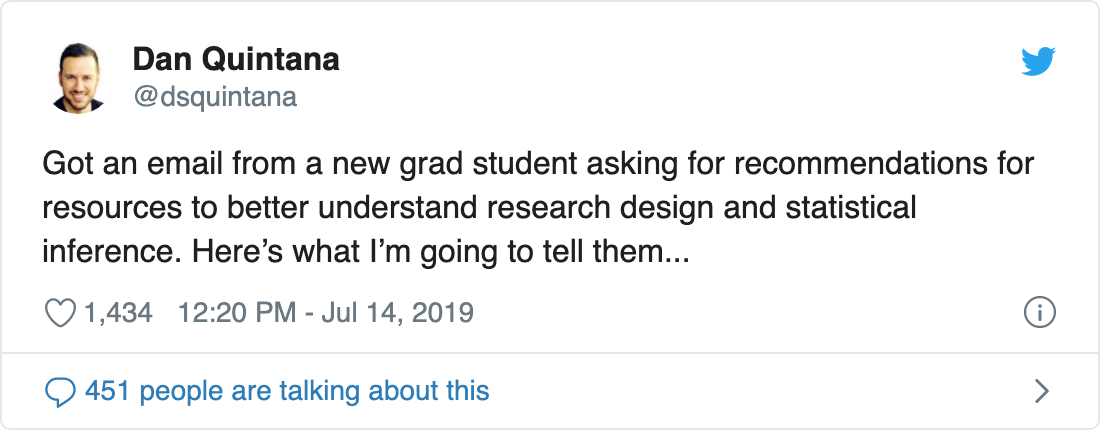
\includegraphics{twitter_book_files/figure-latex/tweet-research-design-1.png}

Peer-review is a task that most of us do, so you can take this opportunity to make a wider commentary about your research topic. For instance, I recently shared a point about power analysis using a peer-review I was conducting.

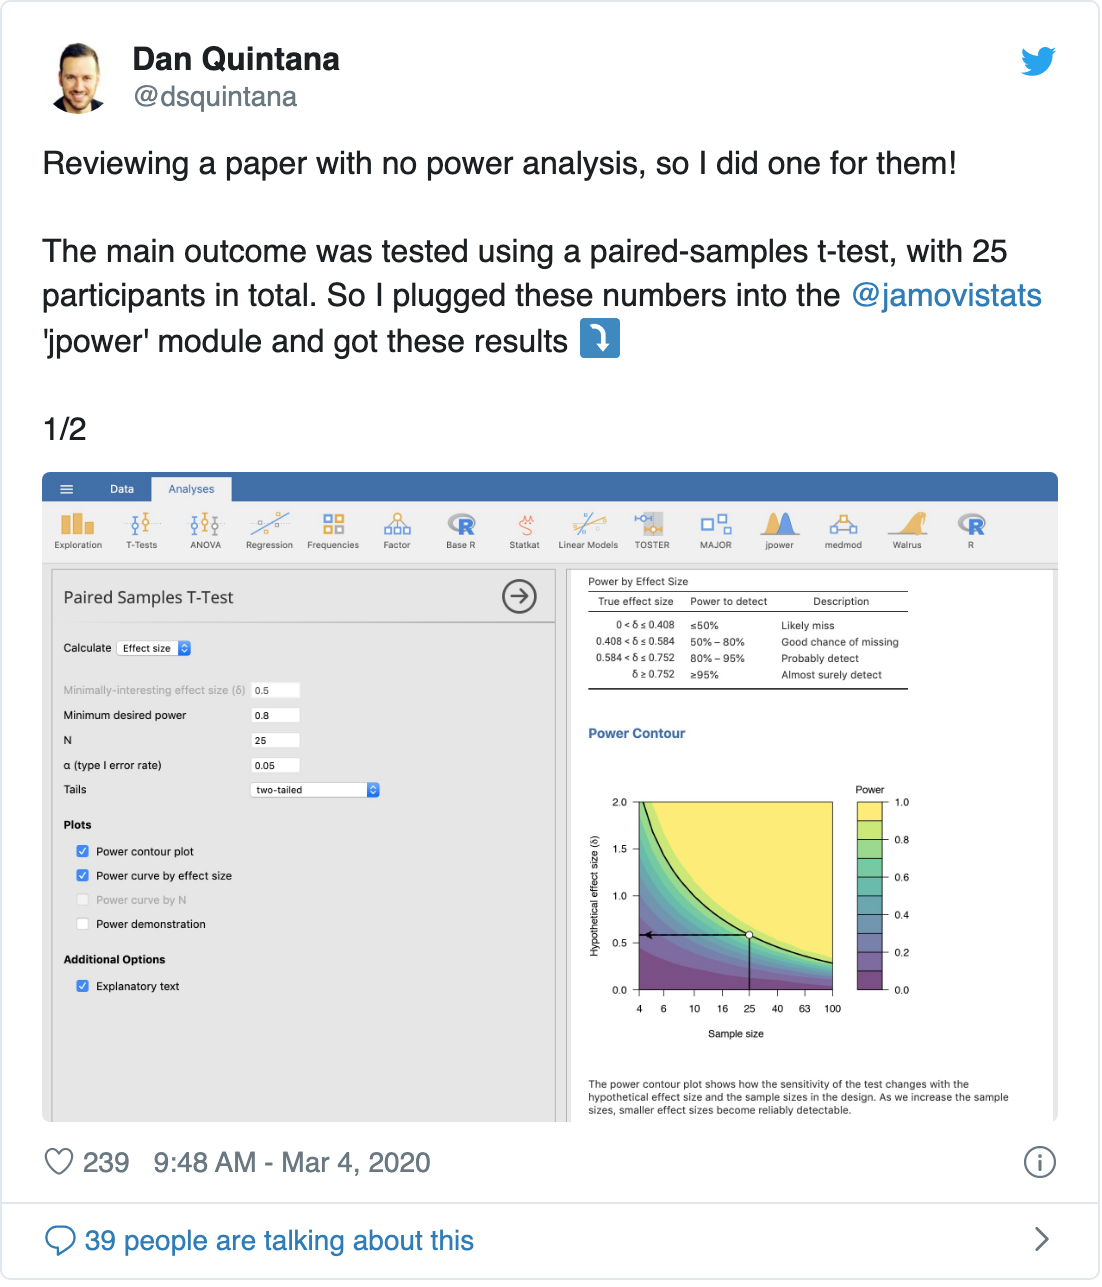
\includegraphics{twitter_book_files/figure-latex/tweet-power-analysis-1.png}

Let's break down this tweet:

\begin{enumerate}
\def\labelenumi{\arabic{enumi}.}
\tightlist
\item
  I used a line break to clearly separate the two parts of this tweet.
\item
  The screenshot image is eye catching (especially the plot) and conveys a lot of information.
\item
  The `down arrow' emoji adds a tiny bit of flair.
\item
  I tagged a tool that I mentioned \href{https://twitter.com/Jamovistats}{@Jamovistats}, so that followers could easily find out more.
\item
  I numbered this tweet ``1/2'', to signal that this is a two-part tweet. My followers will see these two tweets back-to-back, but people who see this tweet as a retweet will now know there is more than one tweet on this topic, and can then check the full conversation.
\end{enumerate}

Of course, if you're going to tweet about peer review you will need to keep things as anonymous as possible! Also consider that the author of the paper may follow you on Twitter or come accross your tweet if it gets retweeted.

You can also tweet about being at the \emph{other end} of the peer review process.


\includegraphics{twitter_book_files/figure-latex/tweet-peer-review-1.png}

Remember, the key is sharing the process of your work, not just the final product.

\hypertarget{intermediate}{%
\chapter{Intermediate Twitter skills}\label{intermediate}}

Here are a few ways that you can lift your Twitter game now that you've got some experience under your belt.

\hypertarget{pinning-a-tweet-to-your-profile}{%
\section*{Pinning a tweet to your profile}\label{pinning-a-tweet-to-your-profile}}
\addcontentsline{toc}{section}{Pinning a tweet to your profile}

Once you've got more than about twenty tweets, you should `pin' one of these tweets to the top of your profile. A pinned tweet will be the first tweet that someone sees when they visit your profile, so use this wisely. Here are some ideas of the types of tweets you should consider pinning to your profile:

\begin{itemize}
\tightlist
\item
  Your latest paper
\item
  Your most important paper
\item
  Information about an upcoming talk
\item
  A summary of your current research project
\item
  An announcement for research participant recruitment
\item
  An image of you doing your job or a text tweet describing aspects of your work
\item
  That you're looking for a new position
\end{itemize}

As for me, I tend to choose what is currently my most important paper. Pinned tweets continue to get likes and retweets long after you originally post them.

\hypertarget{bookmarking-tweets}{%
\section*{Bookmarking tweets}\label{bookmarking-tweets}}
\addcontentsline{toc}{section}{Bookmarking tweets}

While some people ``like'' tweets as a way to bookmark them for later use, Twitter has a specific bookmarking feature. Just click on the share button under a tweet, then click on ``Add Tweet to Bookmarks'', as \href{https://twitter.com/_DaniBeck}{@\_DaniBeck} demonstrates here.

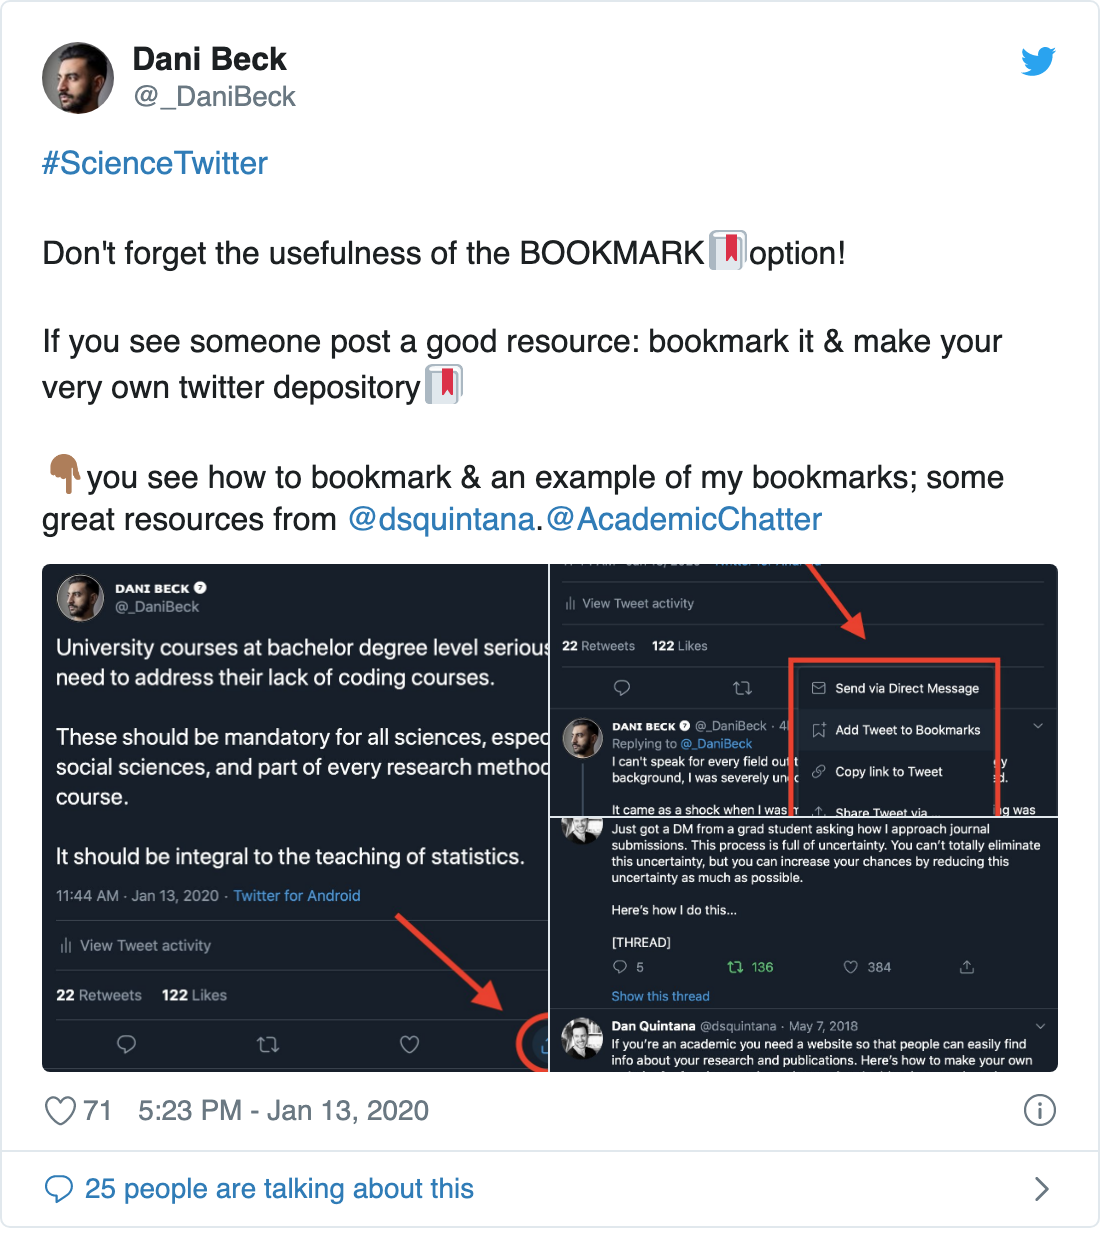
\includegraphics{twitter_book_files/figure-latex/tweet-bookmarking-1.png}

This is a handy feature for when you come across a tweet with a link to an interesting paper but you don't have the time now to read it that precise moment, for instance.

\hypertarget{hashtags}{%
\section*{Hashtags}\label{hashtags}}
\addcontentsline{toc}{section}{Hashtags}

These are useful for categorizing your tweets. One example of hashtag use is that they can organise communities of like-minded people. The \#PhDchat hashtag is a community of PhD students that often post questions and provide support for each other.


\includegraphics{twitter_book_files/figure-latex/tweet-hashtag-1.png}

Hashtags are also useful for organising tweets related to a specific event, like a conference. Many conferences now announce their `official' hashtag that should be used for tweets related to the conference. For many conferences, there are a lot of interesting conversations happening on Twitter, so make use of the conference hashtag by following it and posting your thoughts using the hashtag.

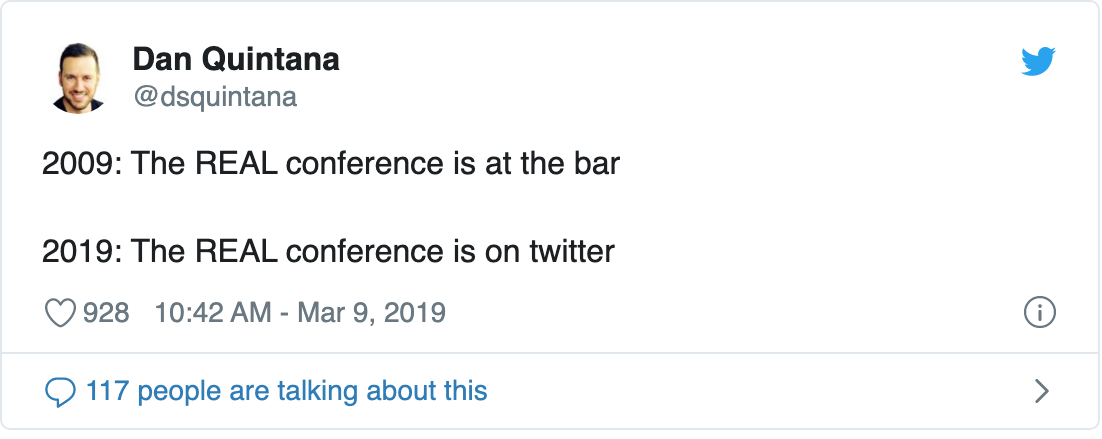
\includegraphics{twitter_book_files/figure-latex/tweet-conference-1.png}

You can also use hashtags in your profile bio, which were mentioned in \protect\hyperlink{beginner}{Chapter 1}, like \href{https://twitter.com/@ChelseaParlett}{@ChelseaParlett}.

\begin{flushleft}
\includegraphics[width=0.8\linewidth]{images/hashtagprofile} \end{flushleft}

By doing this, Chelsea's profile will appear when people search for the hashtags that she has included.

\hypertarget{images}{%
\section*{Images}\label{images}}
\addcontentsline{toc}{section}{Images}

When you post your images, you can tag Twitter usernames in your images. After adding your image, click on ``Tag people''.

\begin{figure}

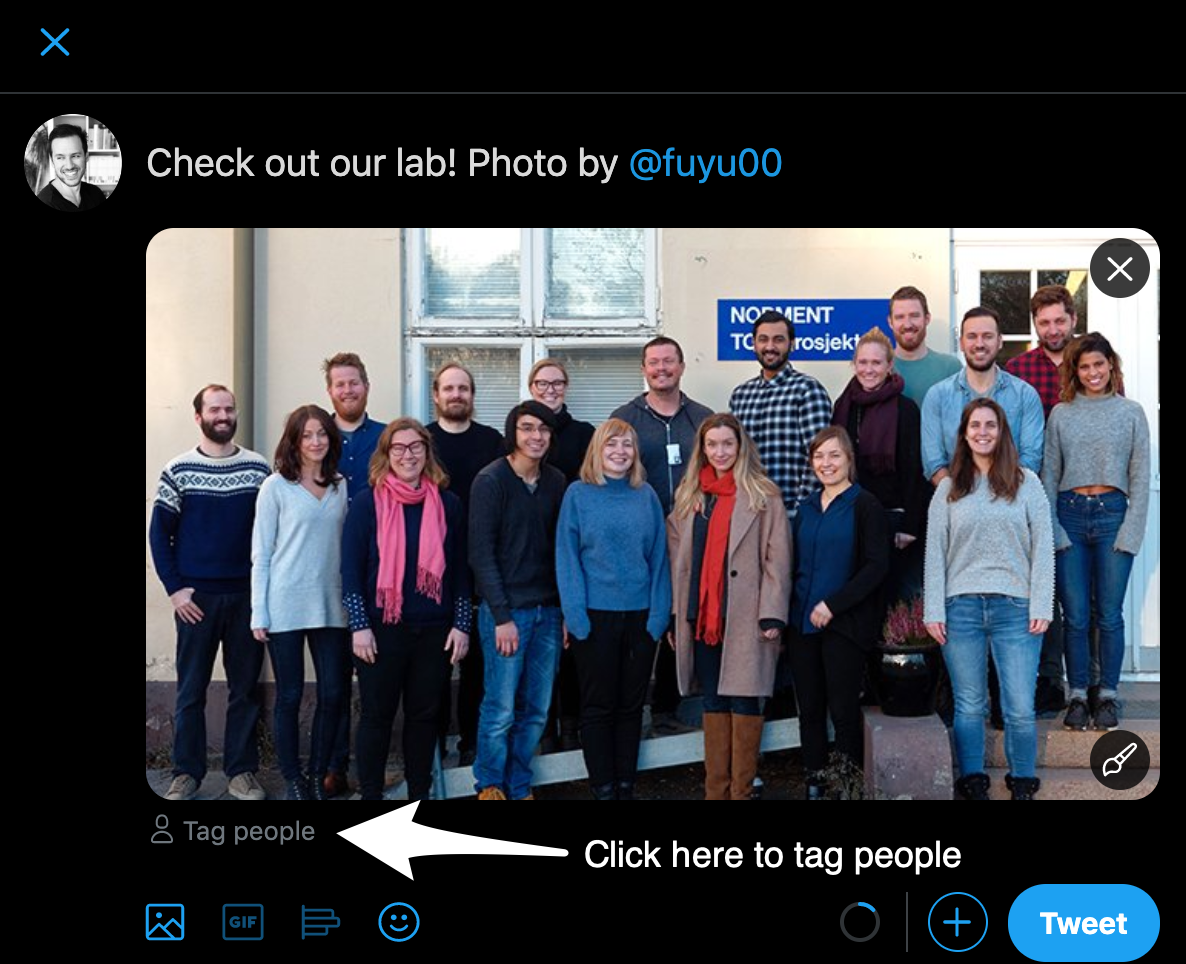
\includegraphics[width=0.8\linewidth]{images/tag} \hfill{}

\caption{Tagging users in photos.}\label{fig:unnamed-chunk-12}
\end{figure}

Tagging photos has a few advantages. First, it saves you a few characters in your tweet as you tag people in the photo instead. Anyone that you tag will be notified that they've been included in a photo. You don't have to use this feature for only tagging pictures of people. For example, you can post a screenshot of the abstract of a new paper and tag the co-authors of your paper.

\hypertarget{twitter-polls}{%
\section*{Twitter polls}\label{twitter-polls}}
\addcontentsline{toc}{section}{Twitter polls}

If you're reading this, you're probably a scientist, so you should understand that Twitter polls are by no means scientific. However, they still provide \emph{some} information and provide a fun alternative to typical text tweets.

\begin{figure}

{\centering 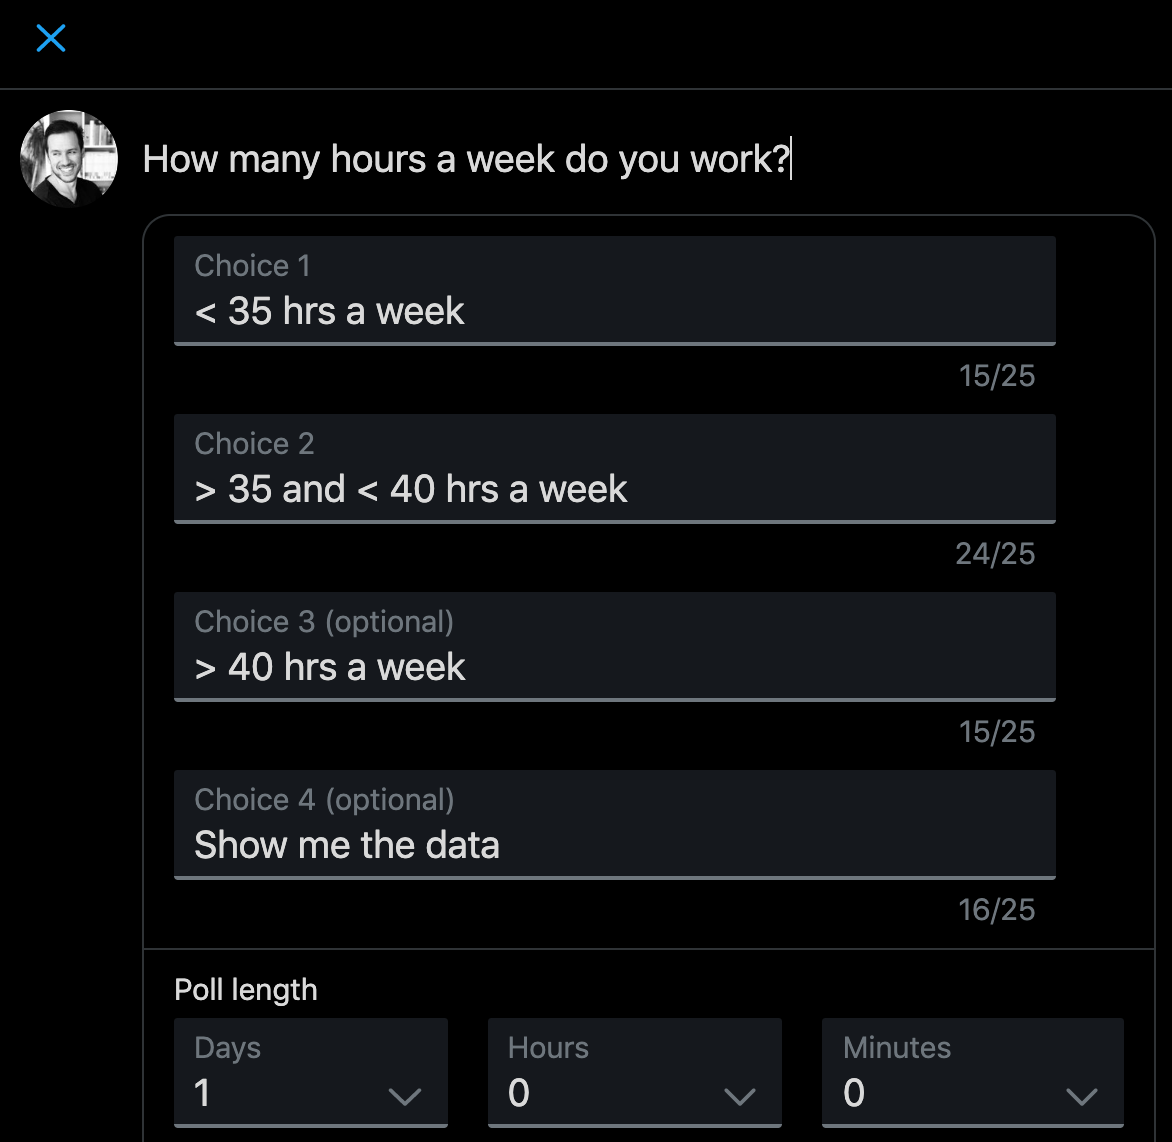
\includegraphics[width=0.8\linewidth]{images/poll} 

}

\caption{A twitter poll}\label{fig:unnamed-chunk-13}
\end{figure}

To improve data quality, people sometimes include a ``Show me the data'' option. This means that people can still see the results without swaying the vote with inaccurate data. You can also set how long the poll should run for. You will get a notification once the poll has closed, so that you can see the final results.

Polls can sometimes start an interesting discussion around the subject of the poll, so consider using this as a conversation starter.

\hypertarget{notifications}{%
\section*{Notifications}\label{notifications}}
\addcontentsline{toc}{section}{Notifications}

If you're easily distracted, I would consider \href{https://help.twitter.com/en/managing-your-account/notifications-on-mobile-devices}{editing your notification settings} or turning then off altogether. It's nice to get that little buzz on your phone or the little red dot on your Twitter browser \href{https://en.wikipedia.org/wiki/Favicon}{favicon}, but every little notification, and the time it takes to regain your focus, adds up over the day.If you're easily distracted by twitter, check out some of the tools mentioned in \protect\hyperlink{care}{Chapter 5}.

\hypertarget{lists}{%
\section*{Lists}\label{lists}}
\addcontentsline{toc}{section}{Lists}

With \href{https://help.twitter.com/en/using-twitter/twitter-lists}{Twitter lists}, you can create unique feeds that \emph{only} contain specific groups of Twitter accounts. This is a useful way of filtering your general feed, which can get quite busy once you start following more than a couple of hundred accounts. You can also subsribe to other user's curated lists.

Here are a few list suggestions if you'd like to make your own:

\begin{itemize}
\tightlist
\item
  Your collaborators
\item
  People in your institution or lab
\item
  Journals and preprint servers
\item
  Scientists that tweet about specific topics (e.g., statistics)
\item
  Non-science interests (e.g., music)
\item
  Accounts that make you laugh
\end{itemize}

These lists can either be public or private, and you don't have to be following accounts that you've added to your list.

\hypertarget{advanced}{%
\chapter{Advanced Twitter skills}\label{advanced}}

\hypertarget{twitter-threads}{%
\section*{Twitter threads}\label{twitter-threads}}
\addcontentsline{toc}{section}{Twitter threads}

You can't say a lot in a 280-character tweet, but you \emph{can} with a Twitter thread, which connects a series of tweets. In principle, there is no limit to how many tweets can go in a thread; however, Twitter will only let you post 20 consecutive tweets in a single instance. I think this is a sensible limit for a thread, but you can always add additional tweets after you've posted your first 20, if you like.

One benefit of using the Twitter app on your smartphone is that you can save your tweets as drafts---this includes threads as well. So, this means that you don't have to write a thread in a single sitting. Simply select ``Cancel'' when writing a tweet, then select ``Save draft''.

\hypertarget{using-a-twitter-thread-to-announce-a-new-paper}{%
\subsection{Using a twitter thread to announce a new paper}\label{using-a-twitter-thread-to-announce-a-new-paper}}

Threads are a great way to announce a new paper, as you can say much more than if you were posting a single tweet. I think threads are a much better way to announce your new papers than a blog post, because they're quicker to write and are more likely to be shared. Unless you add an approximate reading time for your blog posts, people don't know what to expect when they see a link to a blog post in Twitter. But threads are typically no longer than 20 tweets (and usually shorter), so people are more likely to start reading. In addition, you never know which tweet in your thread people will find particularly interesting. If you have a 20-tweet thread, then you have 20 tweets that can be potentially retweeted.

For more on why you should write threads, check out this thread.

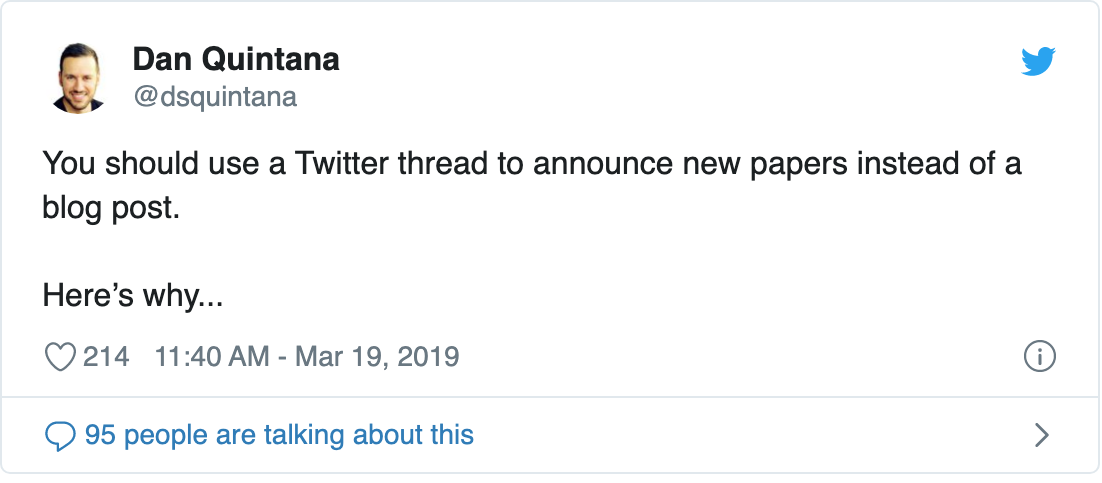
\includegraphics{twitter_book_files/figure-latex/tweet-why-thread-1.png}

\hypertarget{how-to-write-a-thread}{%
\subsubsection{How to write a thread}\label{how-to-write-a-thread}}

Here I've selected ten tweets out of a twenty-five-tweet thread I used to summarise a new paper.

Let's start with the first tweet. This is the introduction, which includes a link to the actual paper and four images from the paper. I also tagged the journal, so that they could be notified of the tweet and hopefully retweet it from their account. I also note that this is a thread, at the bottom of the tweet, so that readers know what to expect.

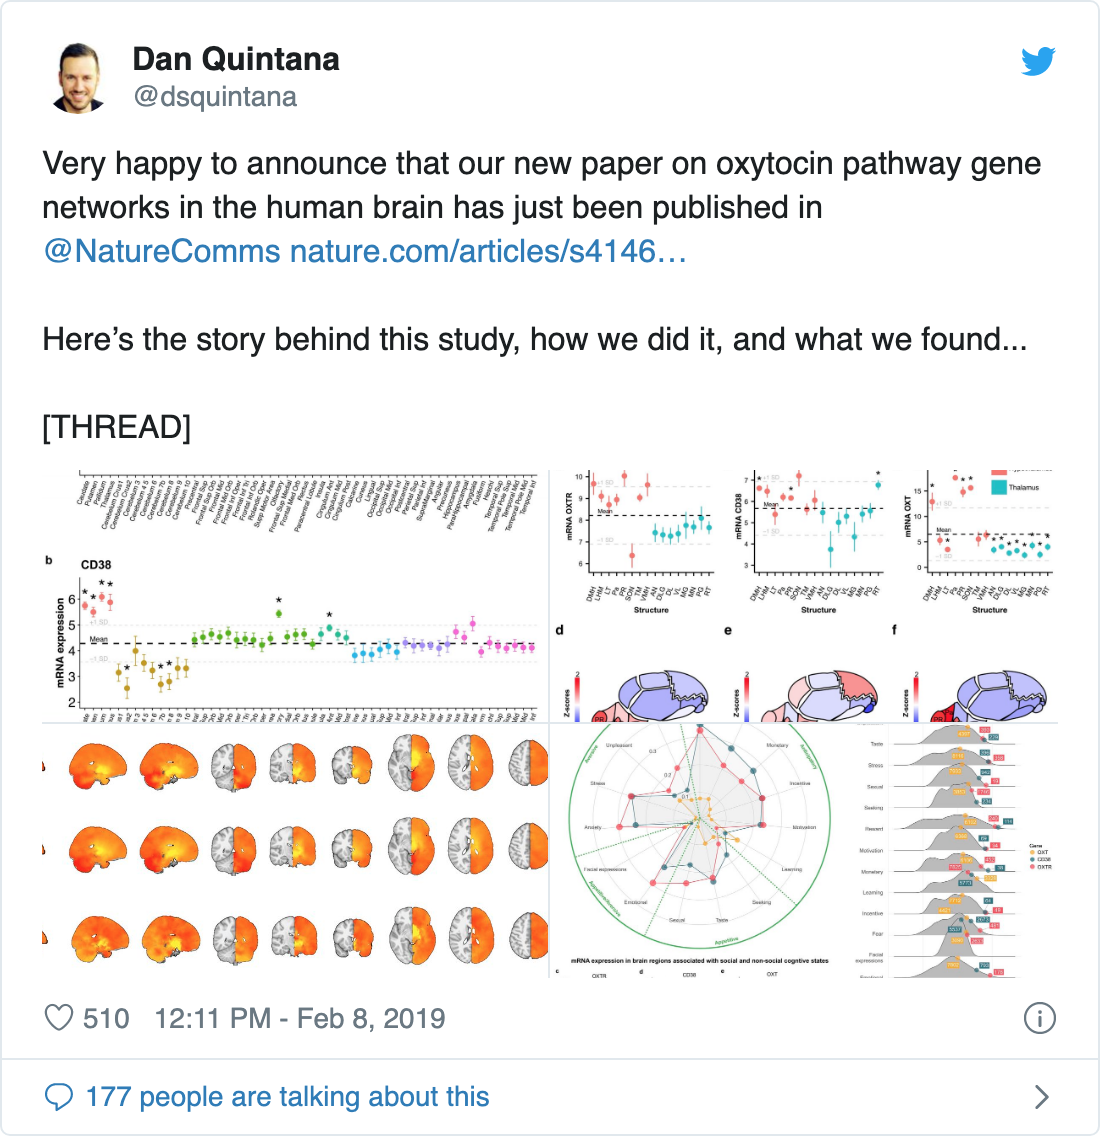
\includegraphics{twitter_book_files/figure-latex/tweet-thread1-1.png}

The next tweet gives a little context as to why I did the study. I added a striking image and a link to the paper it's from if people want to read more.

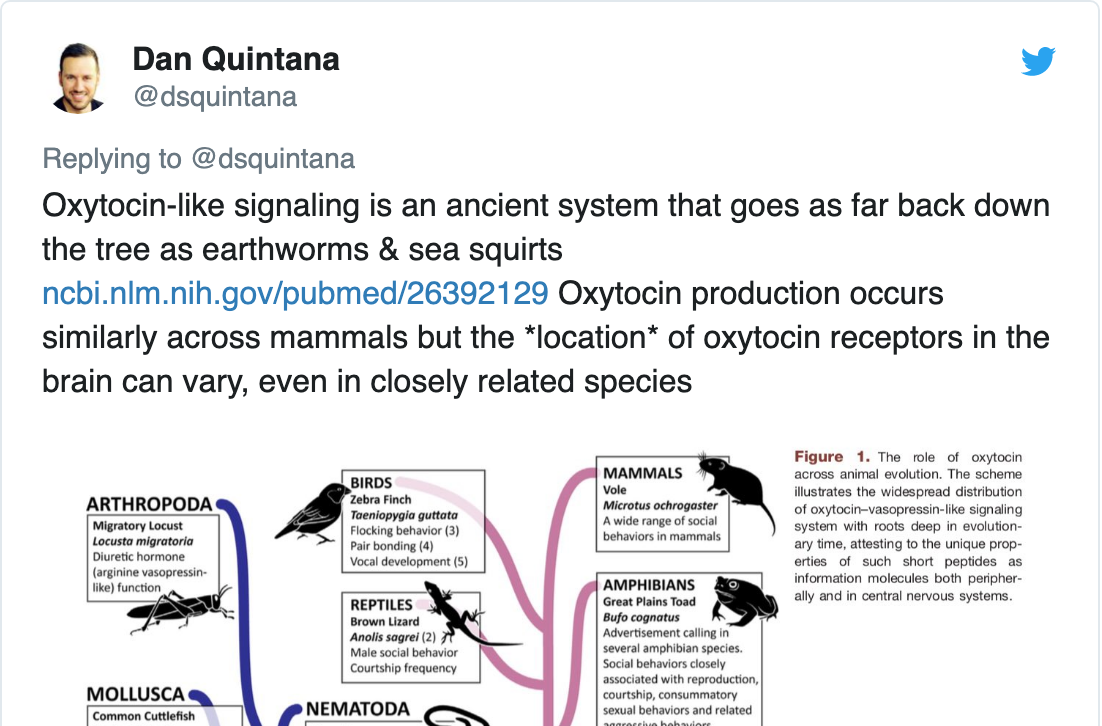
\includegraphics{twitter_book_files/figure-latex/tweet-thread2-1.png}

This tweet explains the story behind the paper idea and acknowledges the team behind the project. I also tag the source of the dataset that I used and my co-authors.


\includegraphics{twitter_book_files/figure-latex/tweet-thread3-1.png}

This tweet covers some of the methods for our analysis.

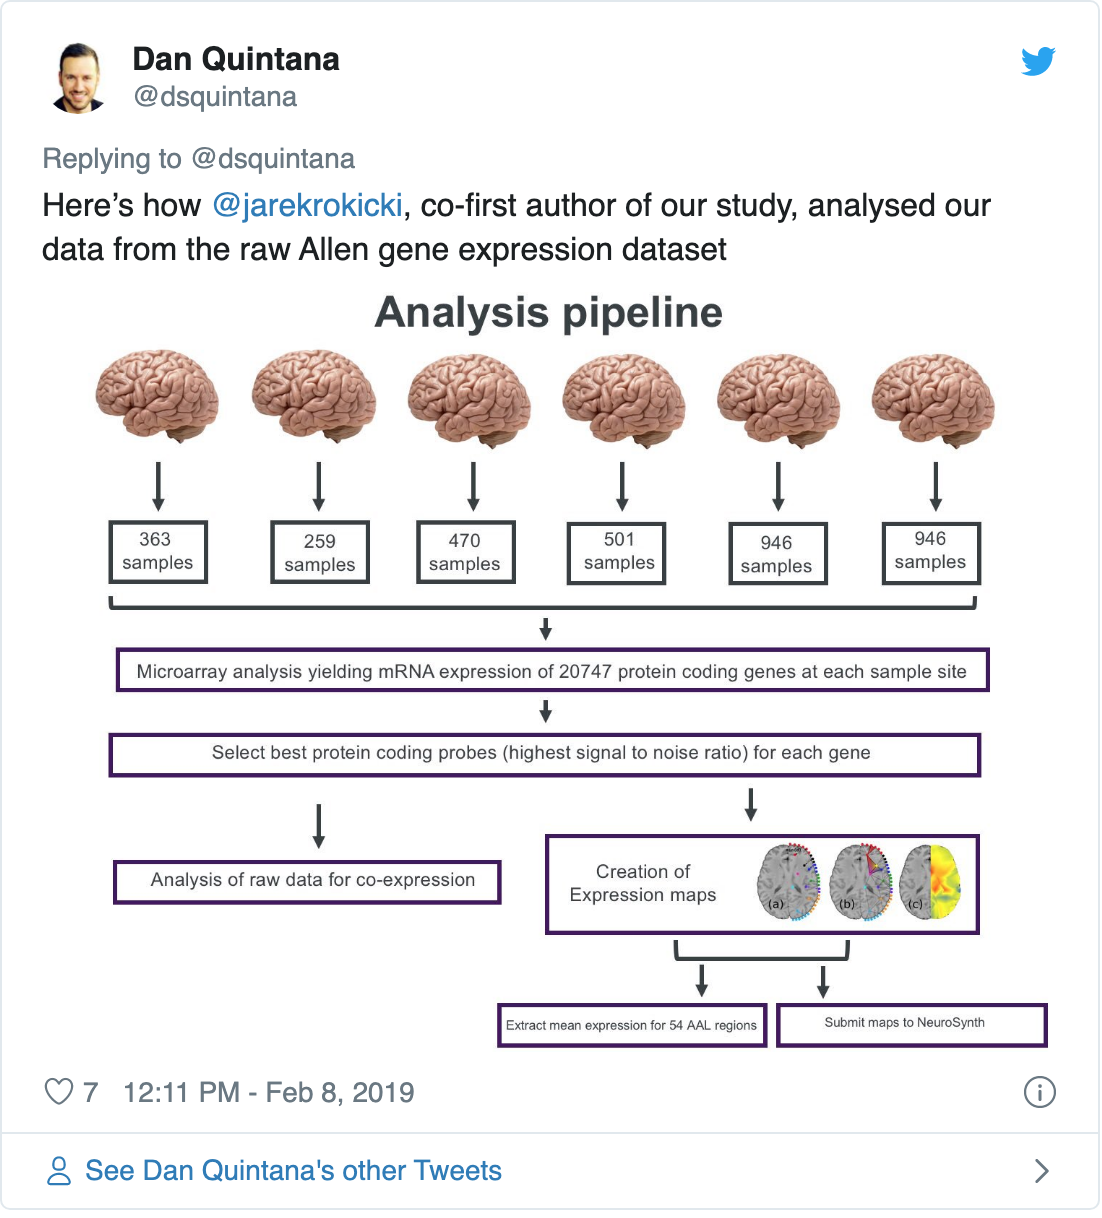
\includegraphics{twitter_book_files/figure-latex/tweet-thread4-1.png}

These two tweets describe some of the results of the paper, via some figures from the paper.

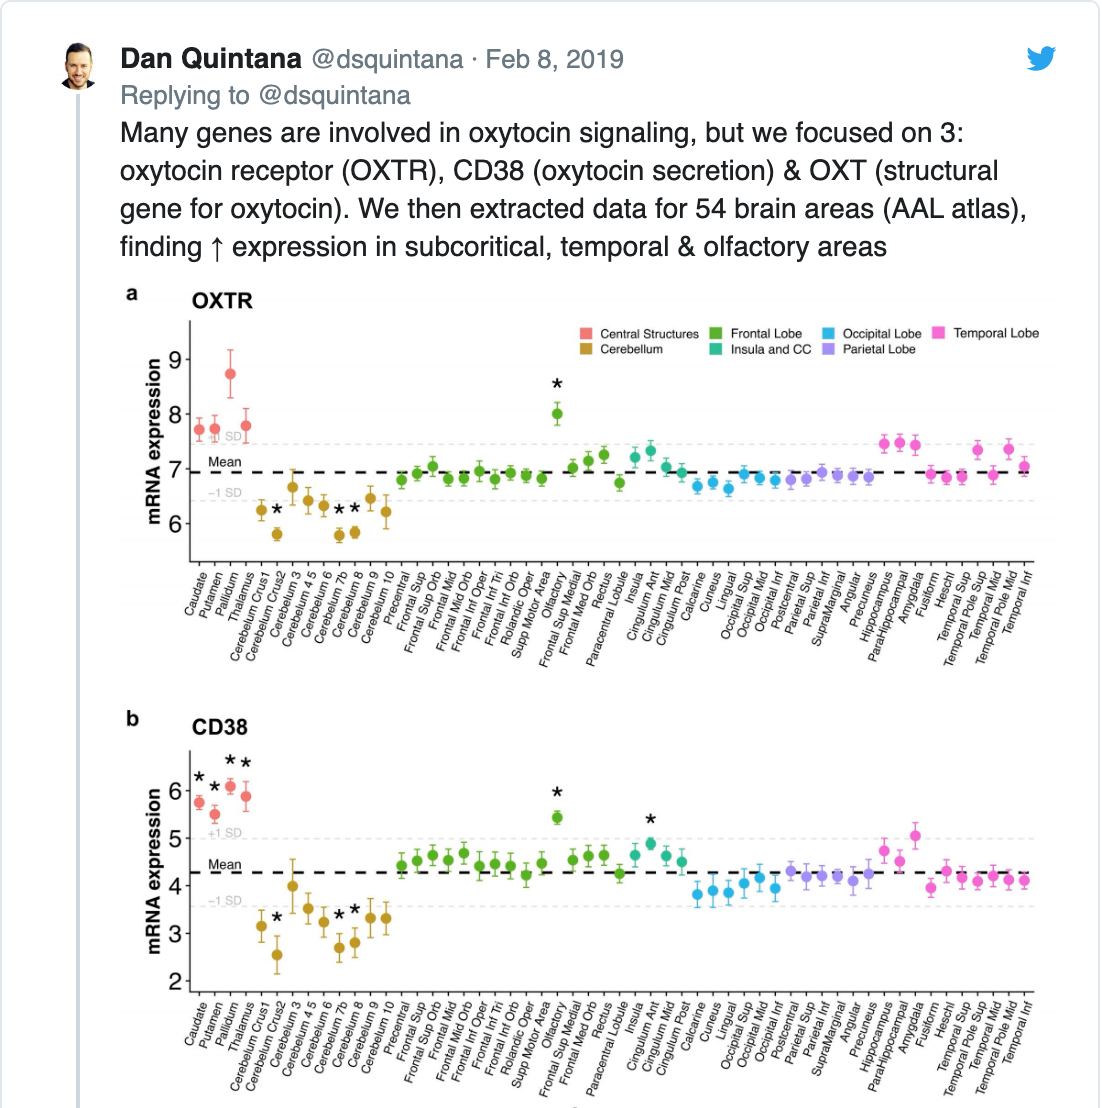
\includegraphics{twitter_book_files/figure-latex/tweet-thread5-1.png}

These two tweets describe some of our methods, including a link to the tool I used (i.e., NeuroSynth) and the paper describing this tool.

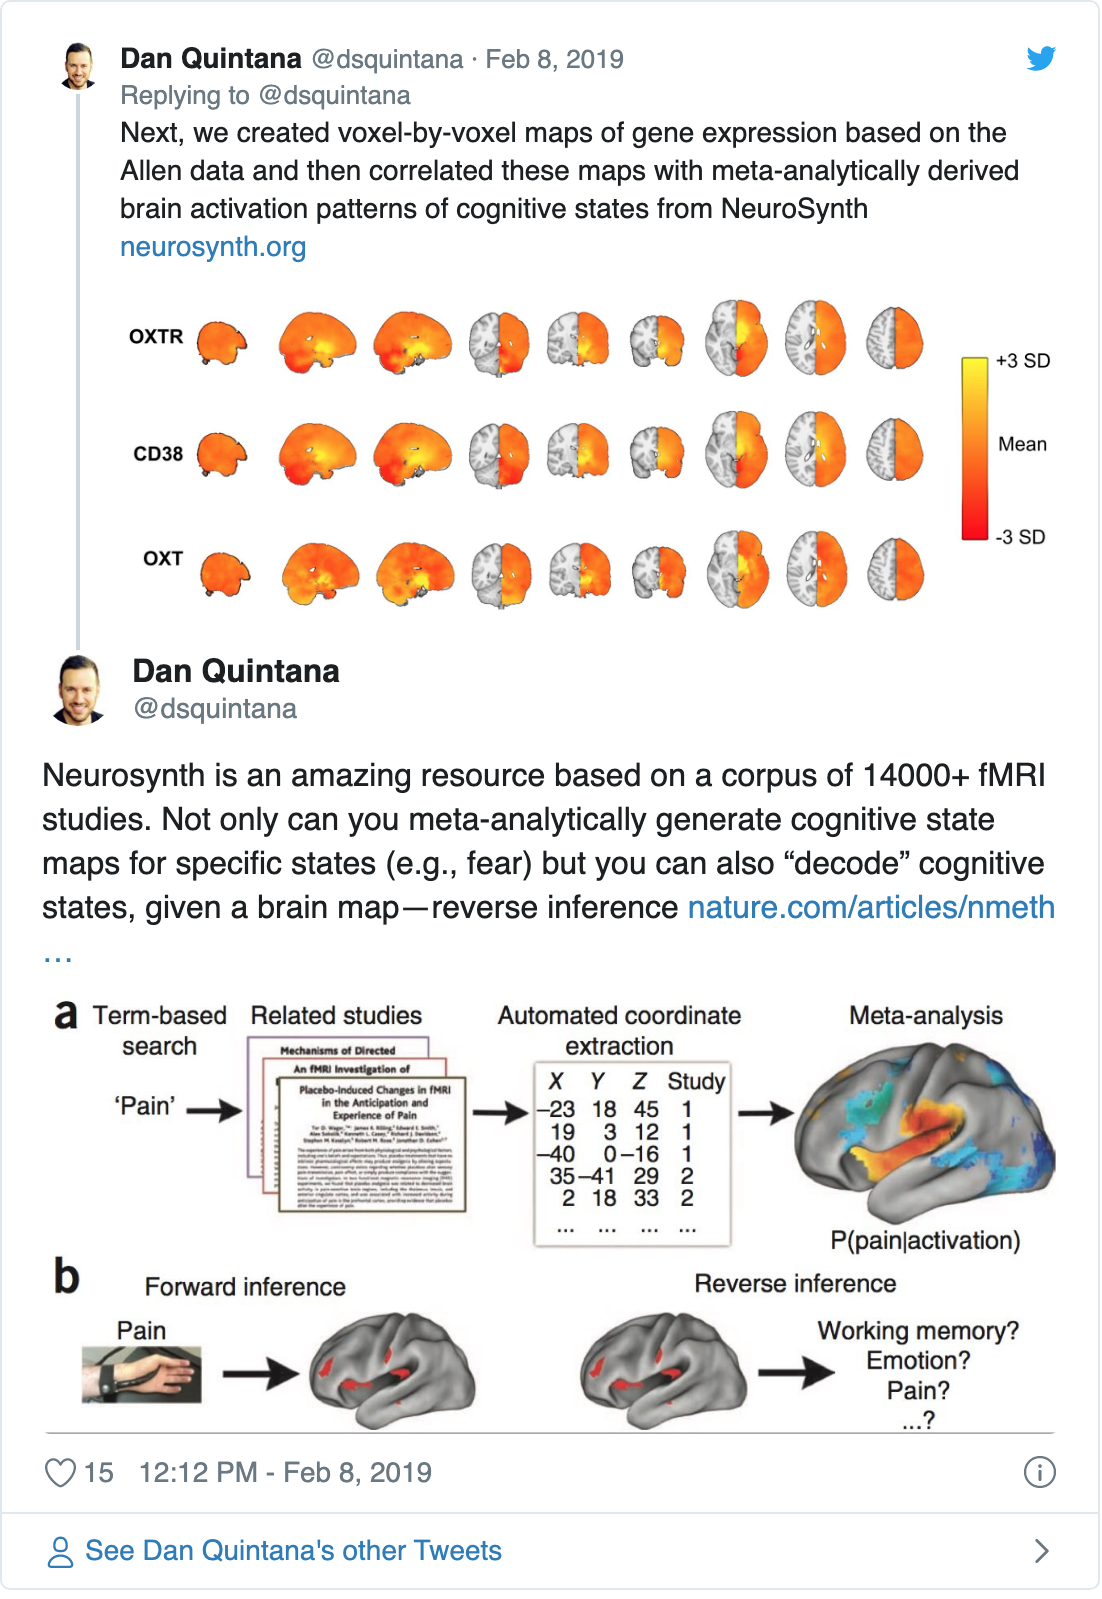
\includegraphics{twitter_book_files/figure-latex/tweet-thread6-1.png}

In this tweet, I acknowledge my inspiration for the study in the first place, to give a little more context.

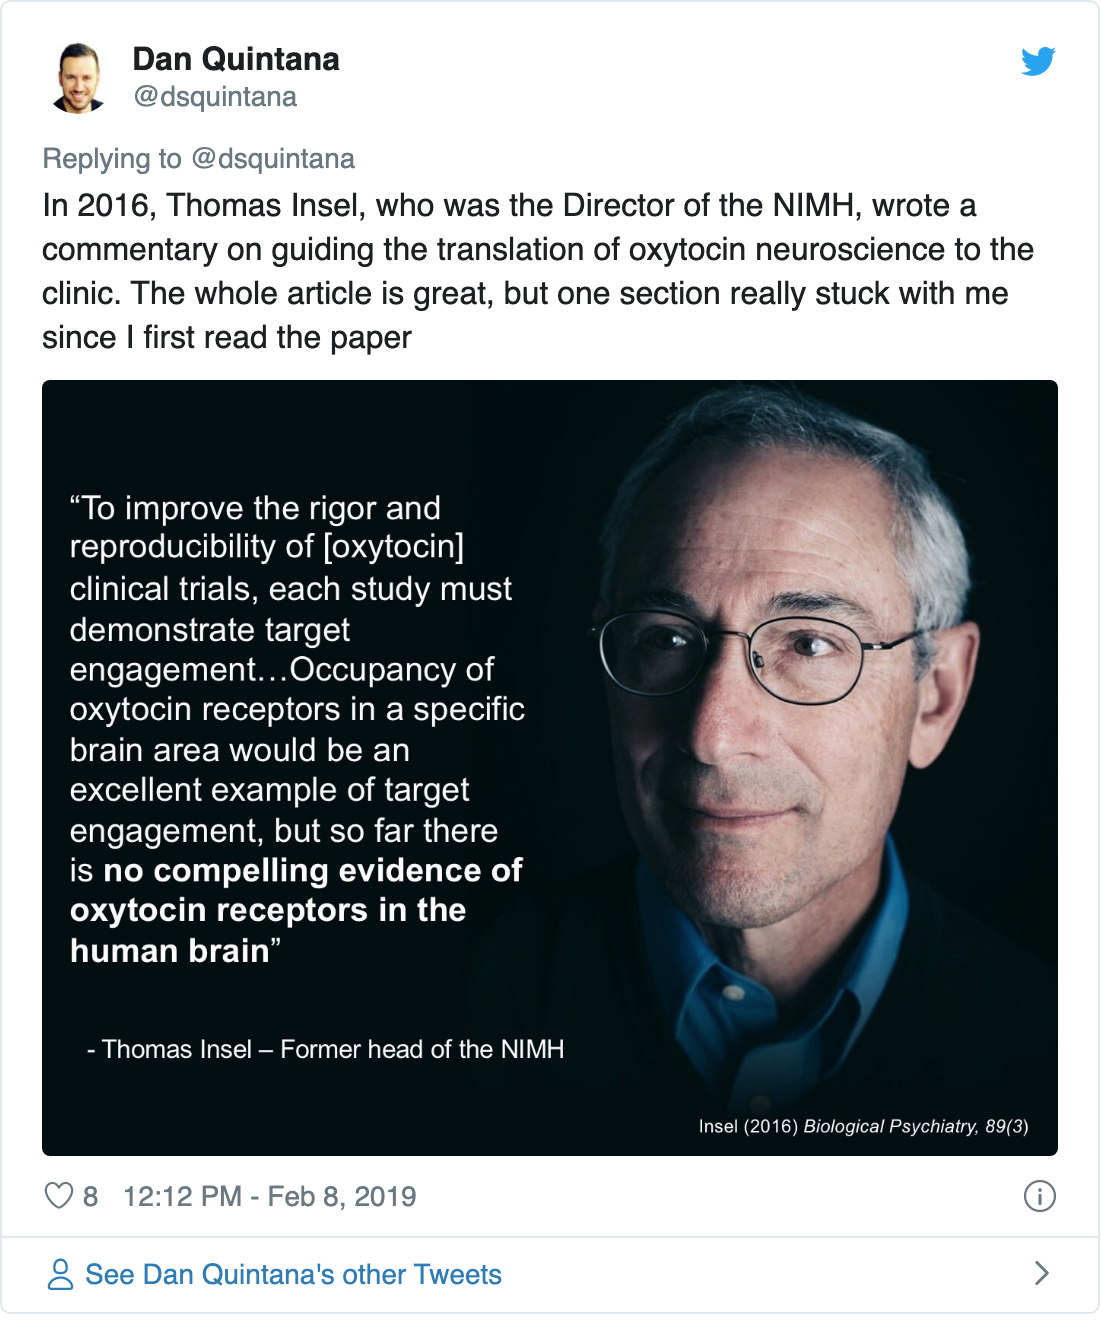
\includegraphics{twitter_book_files/figure-latex/tweet-thread7-1.png}

Finally, I provide a summary and I thank my team again (this paper was \emph{truly} a team effort).

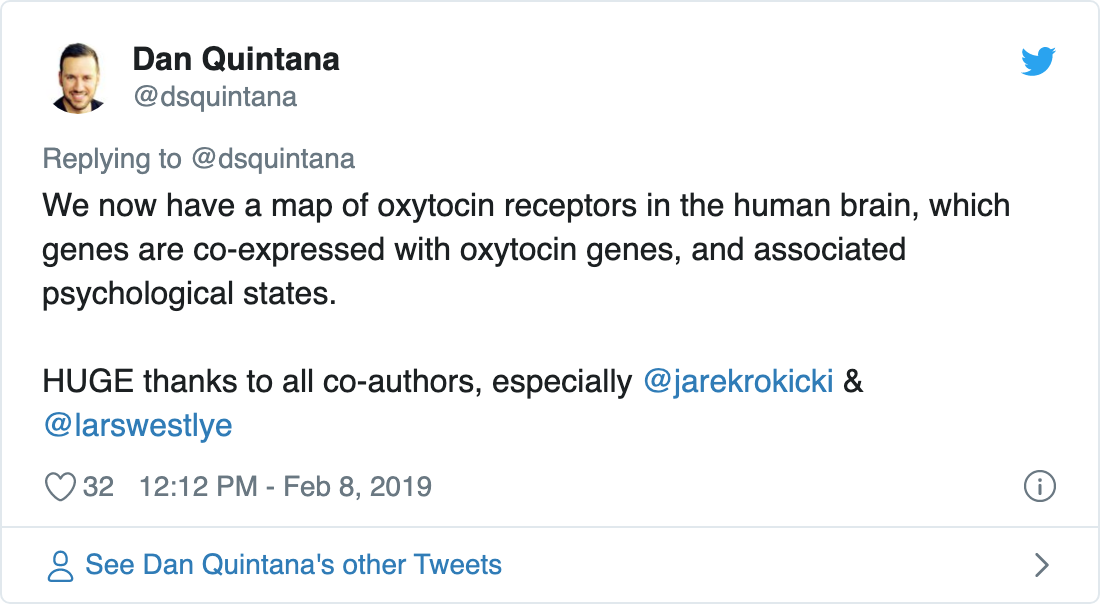
\includegraphics{twitter_book_files/figure-latex/tweet-thread8-1.png}

Before moving to the next section, here's a final tip for your threads: To increase the chances that people will share more individual tweets from your threads, do your best to write each tweet so that it can stand together on its own.

\hypertarget{going-viral}{%
\section*{Going viral}\label{going-viral}}
\addcontentsline{toc}{section}{Going viral}

It's almost impossible to predict which tweets will go viral, so don't spend time trying to make a viral tweet. I made the following tweet on a whim, thinking a few psychological scientists who are familiar with the \href{https://en.wikipedia.org/wiki/Rabbit\%E2\%80\%93duck_illusion}{rabbit-duck illusion} would find this funny. I was spectacularly wrong.

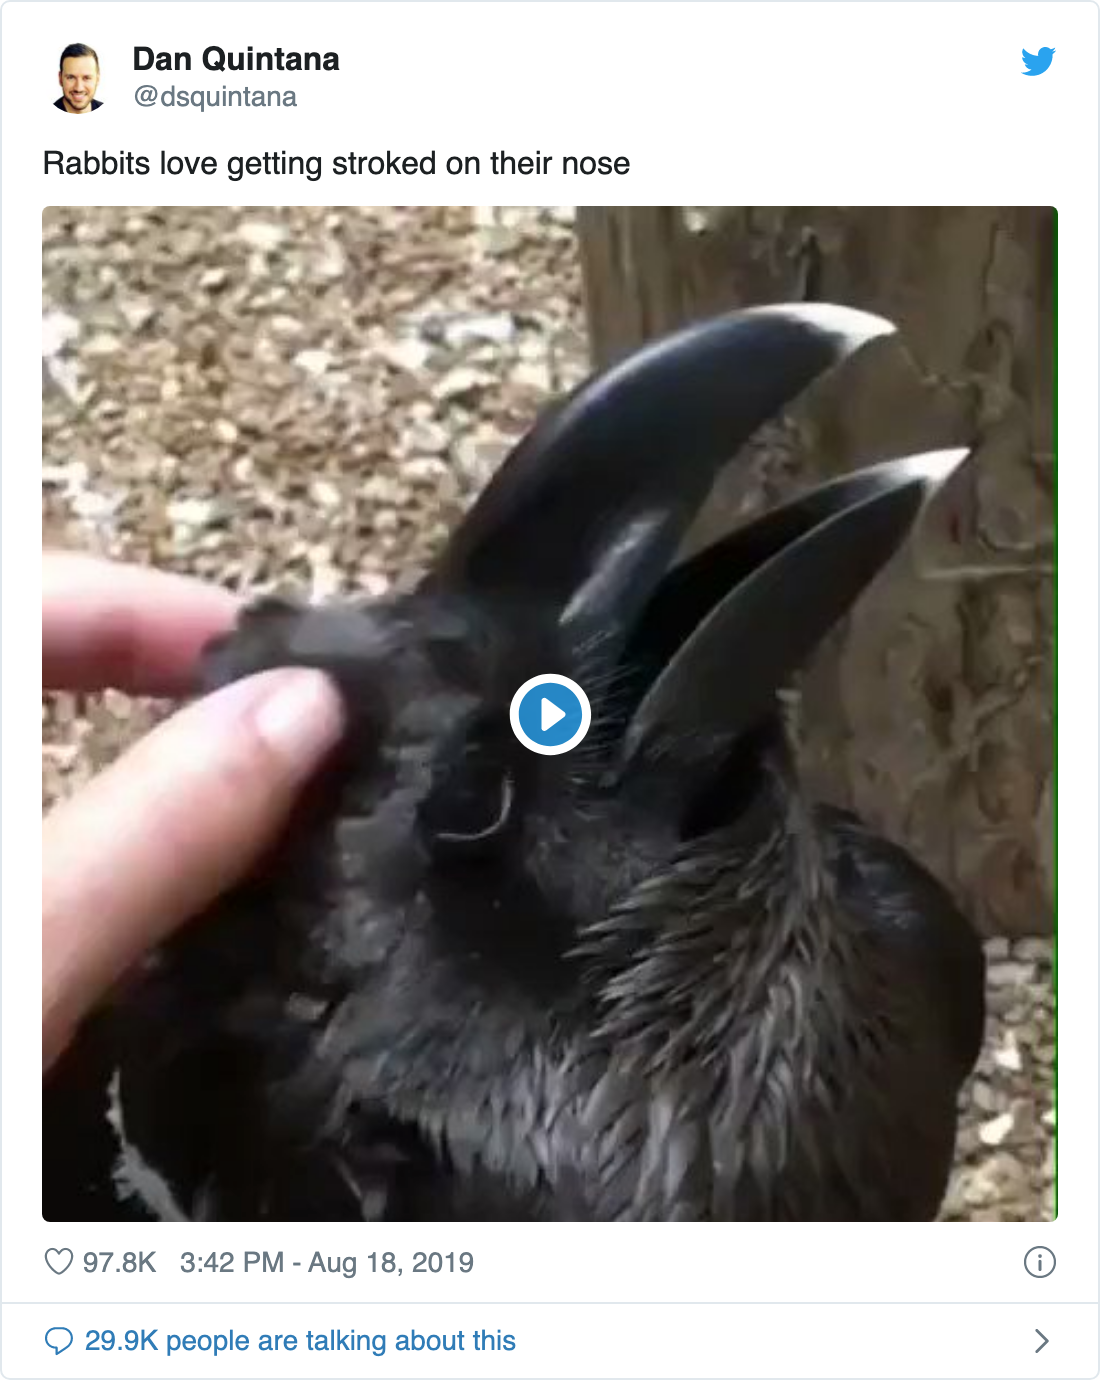
\includegraphics{twitter_book_files/figure-latex/tweet-viral-1.png}

While viral tweets have the upside of getting you a few more followers, Twitter will be essentially unusable for you during this period, as your notifications will be \textbf{flooded}. It's typically tweets that cover general topics that go viral, so you probably won't gain many new followers who are actually interested in your science---but if you're lucky you might get a few. I have found that the further your tweet travels outside of your network, the more \emph{unusual} the responses. You may also get a few nasty tweets as well, which I cover in the \protect\hyperlink{care}{next chapter}.

\hypertarget{making-your-own-gifs}{%
\section*{Making your own GIFs}\label{making-your-own-gifs}}
\addcontentsline{toc}{section}{Making your own GIFs}

GIFs get a lot of attention. For instance, instead of just posting a static image of your paper, you can create a GIF that scrolls through your paper. Of course, you could post this as a video, but people often expect audio when they come across a video. GIFs don't have audio and continually loop. There is a huge library of GIFs online and you can also \href{https://help.twitter.com/en/using-twitter/tweeting-gifs-and-pictures}{search for GIFs} directly in Twitter when composing a tweet.

If you would like to make GIFs on your desktop, I recommend the \href{https://gfycat.com/gifbrewery}{GIF Brewery app} (Mac only), as this gives you lots of options for making GIFs. For your smartphone, I recommend \href{https://imgplay.net/}{ImgPlay} (iOS and Android). The best part of this app is that you can squeeze the size of your GIFs to under the 5MB Twitter limit. You can't do this with GIF Brewery app, and you'll have to sometimes play around with the settings to get your GIF under the 5MB limit.

\hypertarget{getting-your-tweet-back-in-the-feed-again}{%
\section*{Getting your tweet back in the feed again}\label{getting-your-tweet-back-in-the-feed-again}}
\addcontentsline{toc}{section}{Getting your tweet back in the feed again}

No matter where you are in the world, some of your followers will be asleep when you tweet. This means that they might miss your tweet. Don't think too much about ``timing'' your tweets. However, if you've tweeted something important, like a new paper, there are ways to ``re-introduce'' your tweets to your user's feeds.

\textbf{1. Retweeting your original tweet.} I would keep this to minimum, as this is the digital equivalent of patting yourself on the back, but this is fine occasionally.

\textbf{2. Replying to your own tweet with a tweet containing additional information.} By doing this, your followers will see your original tweet (despite the fact it was tweeted in the past) and the new tweet.

\hypertarget{sharing-your-replies}{%
\section*{Sharing your replies}\label{sharing-your-replies}}
\addcontentsline{toc}{section}{Sharing your replies}

If you've written a reply to someone's tweet, the only time it will appear in someone else's feed is if they follow both you and the person you replied to, or if the twitter algorithm somehow pushes this tweet into people's feed if it's produced a lot of likes or retweets. However, if you want more people to see it, you can retweet that particular reply tweet.

\hypertarget{analytics}{%
\section*{Analytics}\label{analytics}}
\addcontentsline{toc}{section}{Analytics}

With the analytics feature, you can see how your individual tweets are performing in terms of impressions (i.e., how many people saw your tweet) and engagements (i.e., How people interacted with your tweet). Here's an example of the types of engagement you can measure.

\begin{figure}

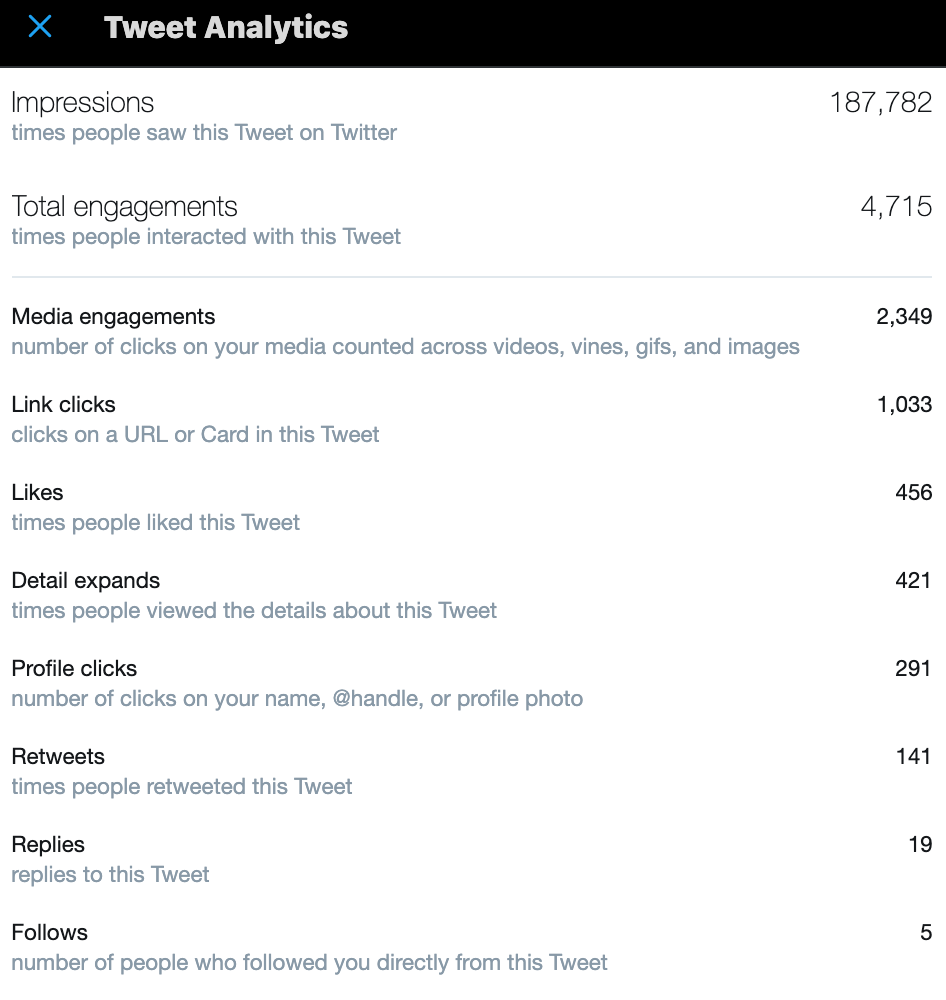
\includegraphics[width=0.8\linewidth]{images/analytics} \hfill{}

\caption{Using the analytics feature to understand how people are engaging with your tweets}\label{fig:unnamed-chunk-14}
\end{figure}

You shouldn't get too hung up on these numbers, but you can use them as a guide for how people are interacting with your tweets. For instance, you might learn that many people are clicking on the links that you share in your tweets. Or perhaps they're clicking more on the images that you're sharing.

\hypertarget{the-tweetdeck-app}{%
\section*{The Tweetdeck app}\label{the-tweetdeck-app}}
\addcontentsline{toc}{section}{The Tweetdeck app}

This \href{https://tweetdeck.com/}{web app}, which can also be downloaded as a \href{https://itunes.apple.com/gb/app/tweetdeck-by-twitter/id485812721?mt=12}{Mac app}, is Twitter on steroids. You can customise this app with different columns, which can contain your main feed, the feed of a specific user (including yourself), notifications, a specific search term, the tweets you've liked, and your messages.

\begin{figure}

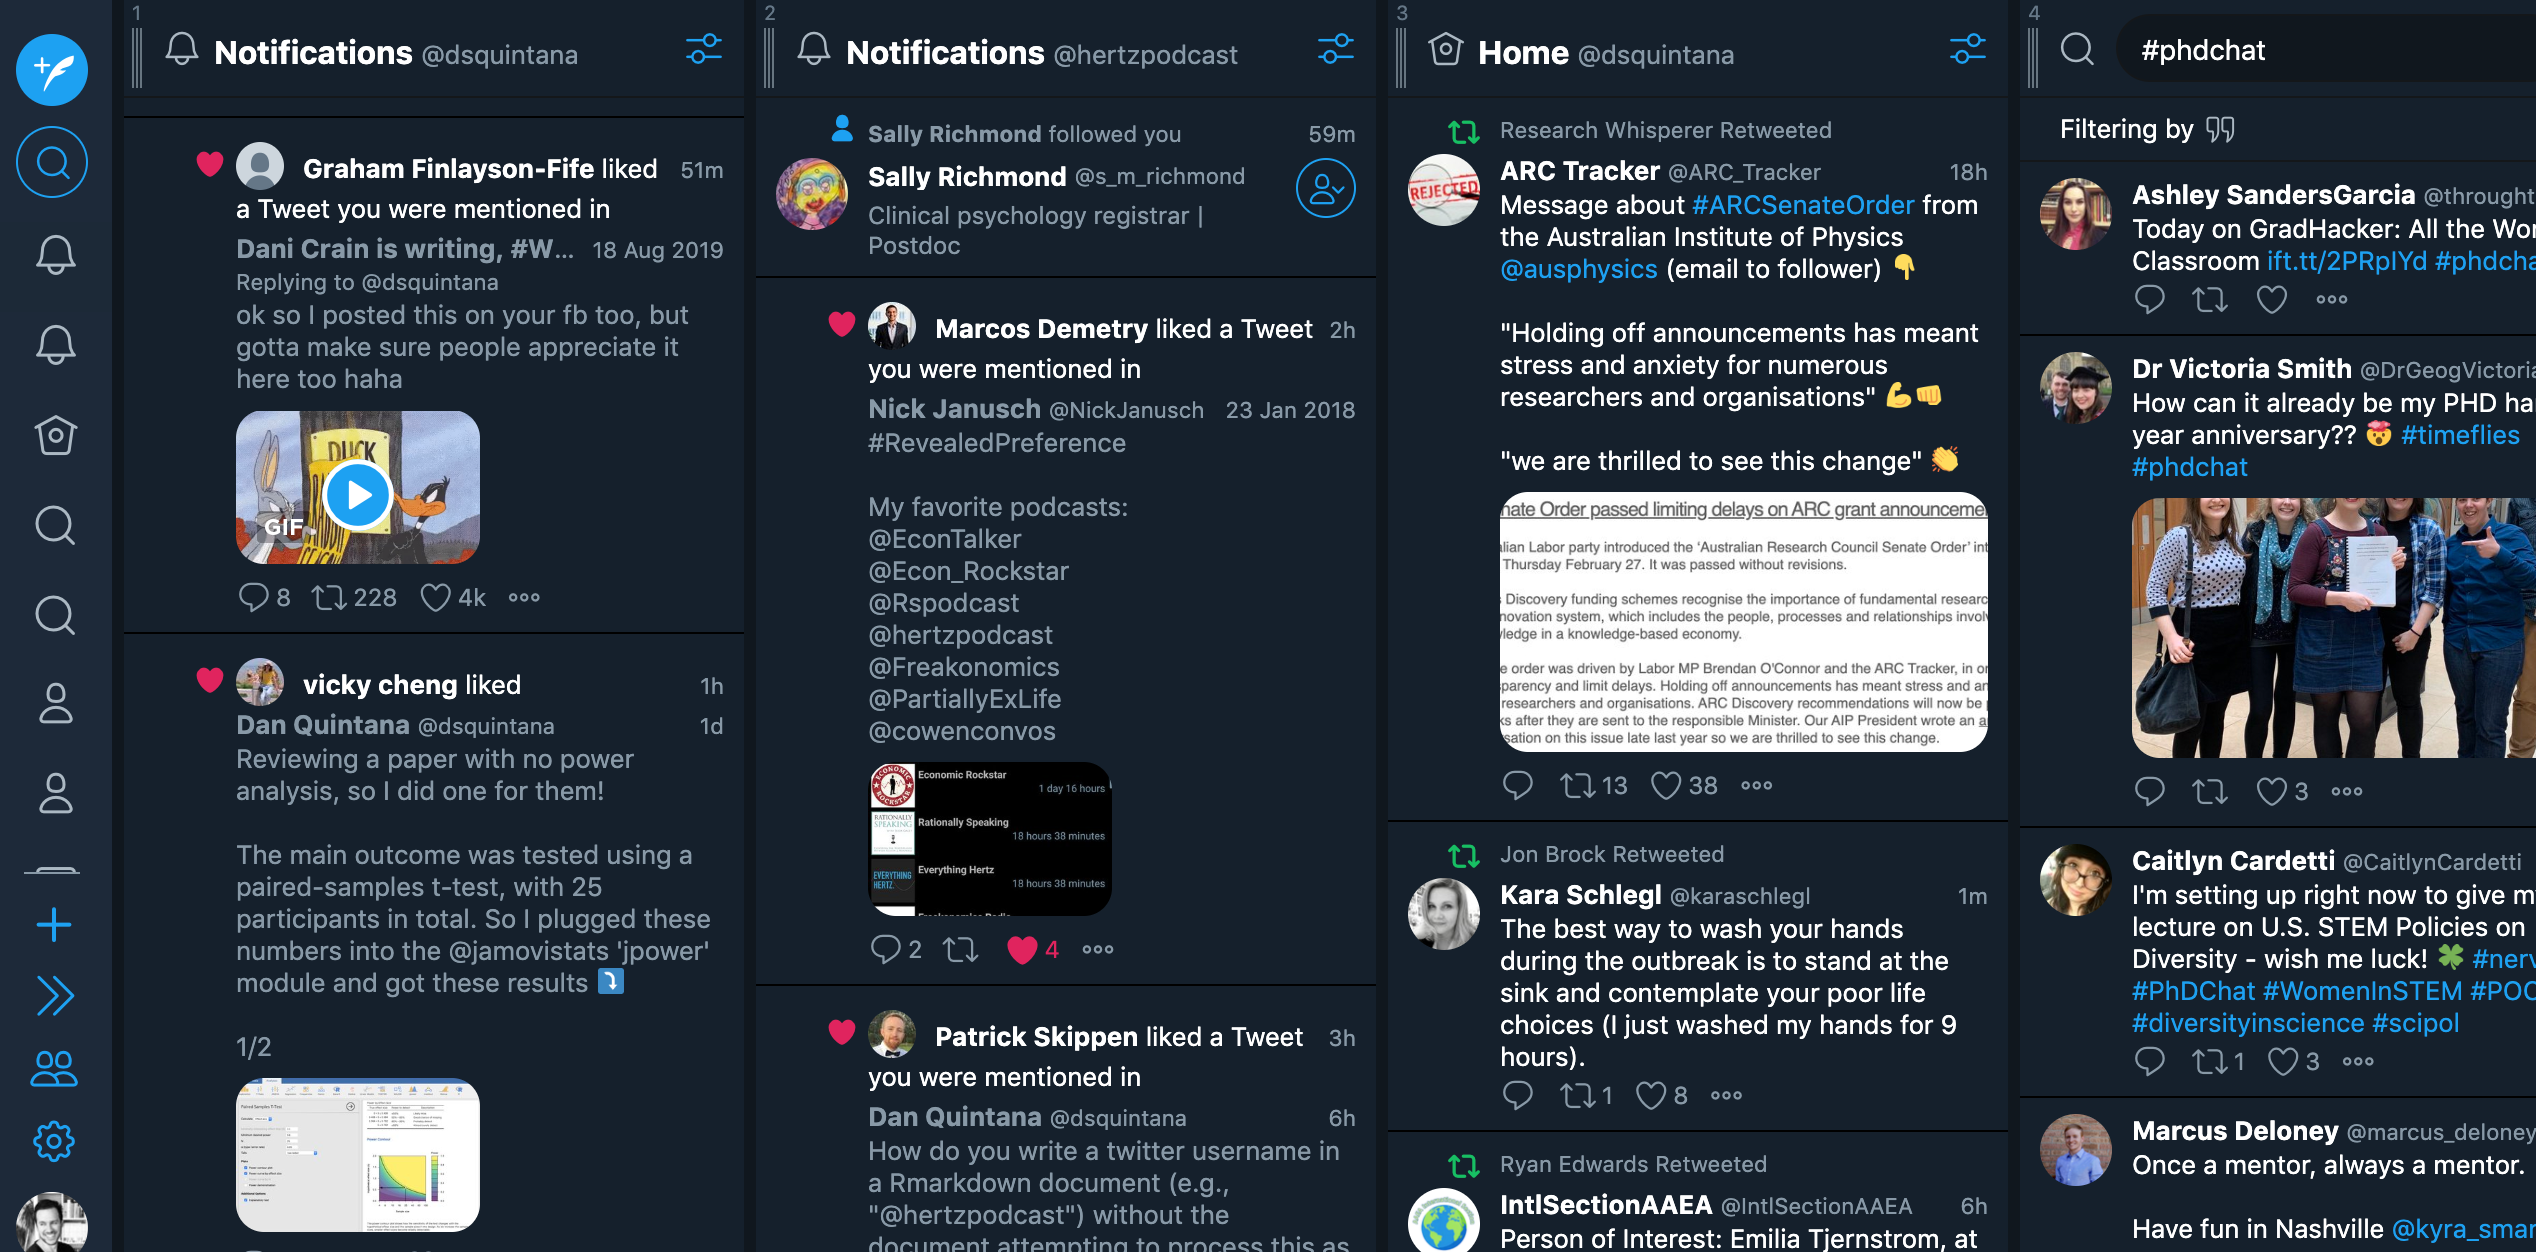
\includegraphics[width=0.8\linewidth]{images/tweetdeck} \hfill{}

\caption{Tweetdeck set up with four columns. Note that the fourth column is for keeping track of the PhDChat hashtag}\label{fig:unnamed-chunk-15}
\end{figure}

Tweetdeck can be particularly useful if you have more than one twitter account (e.g., your individual account and an account for your lab) of if you're following a specific hashtag or search term. You can create a column with any lists that you've put together, which I covered in the \protect\hyperlink{intermediate}{previous chapter}.

But I should warn you, this app can be very addictive because it can show you multiple streams of new information.

\hypertarget{curating-your-labs-twitter-account}{%
\section*{Curating your lab's Twitter account}\label{curating-your-labs-twitter-account}}
\addcontentsline{toc}{section}{Curating your lab's Twitter account}

Having a Twitter account for your lab is a useful way to highlight all the research from your group. It's also a great opportunity to give some exposure to members of your lab, by retweeting their tweets and tagging their usernames. Some labs rotate the curator from week-to-week between lab members, like \href{https://twitter.com/BalesLab}{@BalesLab}.

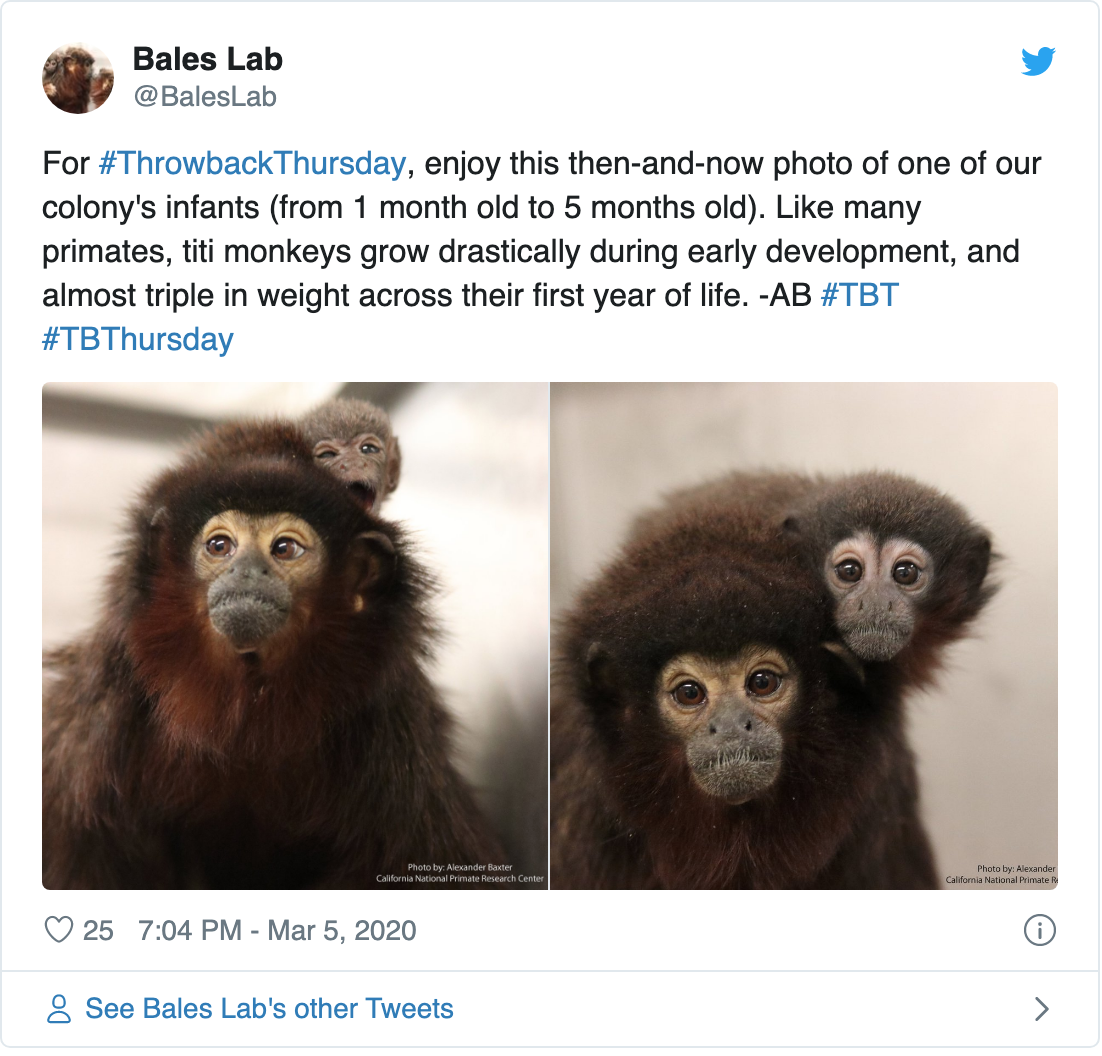
\includegraphics{twitter_book_files/figure-latex/tweet-lab-1.png}

Notice that the tweet is signed off with the initials ``AB''. This is to indicate that the tweet was written by \href{https://twitter.com/Alexer_Baxter}{@Alexer\_Baxter} who is curating the account for the week. This particular tweet is a great example of using a hashtag meme (\#ThrowbackThursday, in which you post a photo from the past) to highlight your work.

It's also a good idea to introduce the curator and to pin this introduction to your lab's Twitter profile, as discussed in the \protect\hyperlink{intermediate}{previous chapter}.

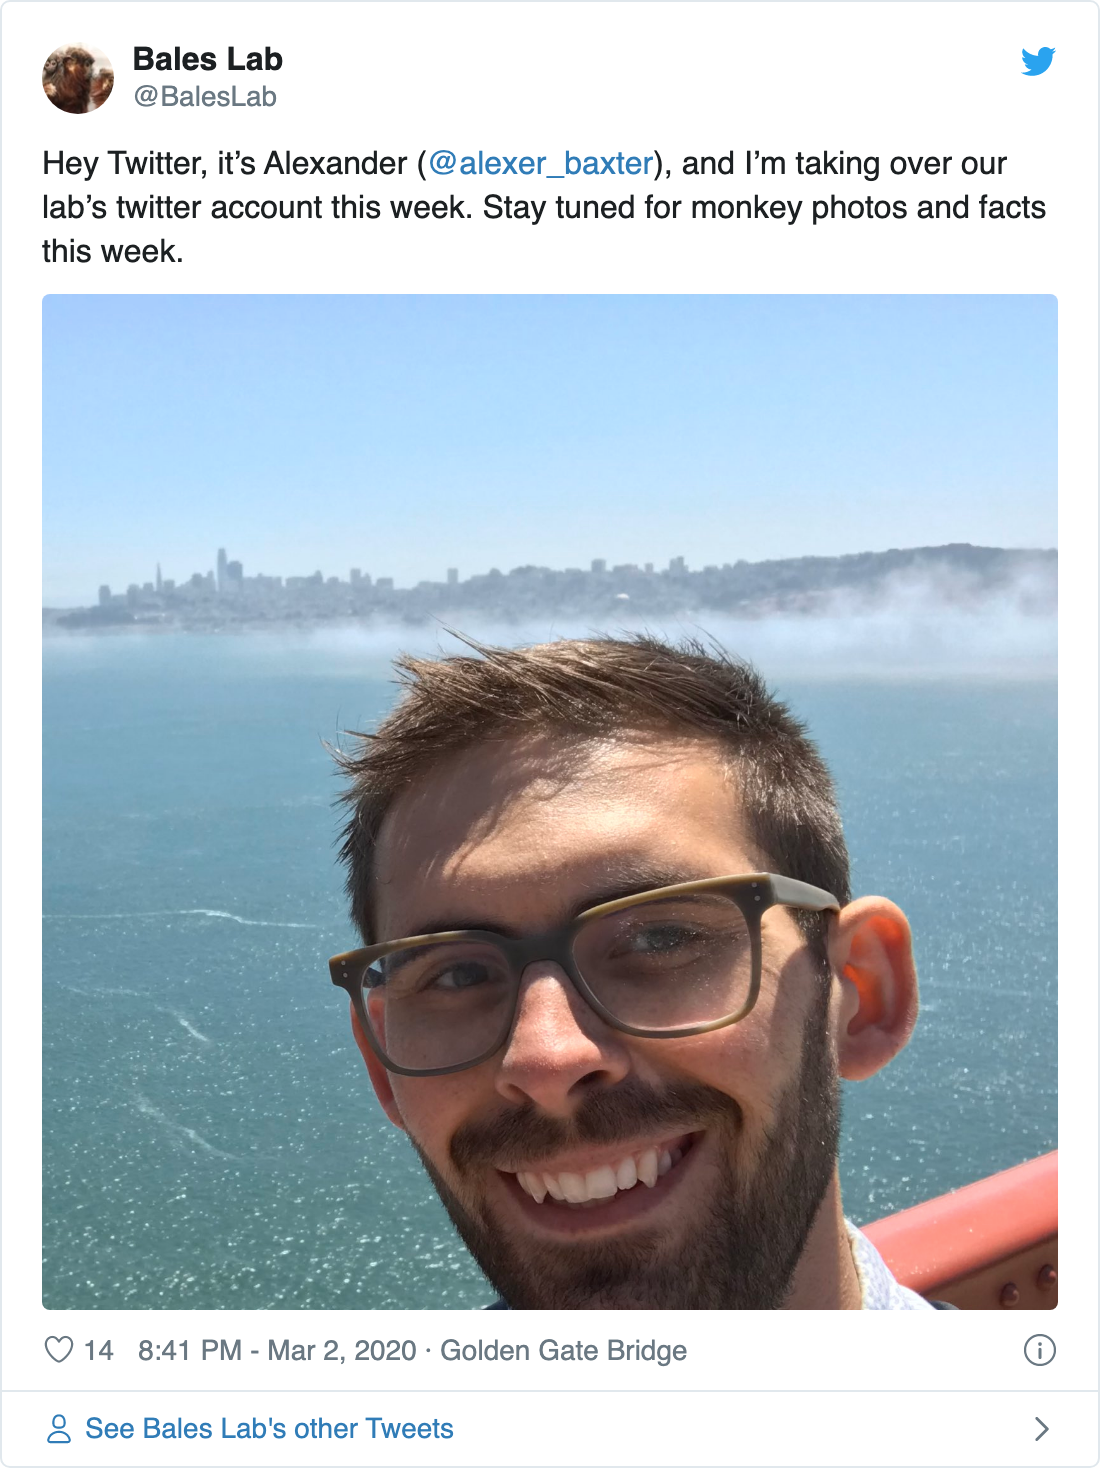
\includegraphics{twitter_book_files/figure-latex/tweet-curator-1.png}

\hypertarget{highlighting-your-work-on-other-platforms}{%
\section*{Highlighting your work on other platforms}\label{highlighting-your-work-on-other-platforms}}
\addcontentsline{toc}{section}{Highlighting your work on other platforms}

Twitter's popularity is not going to last forever (remember MySpace?). It's hard to predict the next big social media platform, but it's either going to be predominantly driven by text, video, or audio. If it's text-based platform, then by getting involved with Twitter \emph{now}, you'll get valuable experience. If you don't want to get involved on Twitter because it's a fad, you'll never get involved on \emph{any} network---they're all fads in the long run. However, if the next big thing is audio or video, then you can use Twitter to highlight your posts on these types of networks.

\hypertarget{video}{%
\subsection{Video}\label{video}}

YouTube is a natural home for any videos you may have of presentations. It's fairly straightforward to save a video of any online presentations that you give via Zoom or Microsoft Teams (just ask for people's permission to record and share beforehand in case they appear in the video).

Even if you don't use YouTube, this is the first point of call for millions of other people when they're wanting to learn about a new topic.

\hypertarget{audio}{%
\subsection{Audio}\label{audio}}

Podcasts have been steadily growing in popularity. While it's relatively straightforward to start your own podcast for very little money (see my \href{https://www.dsquintana.blog/podcast-guide/}{step-by-step guide}), it can be hard for other people to find your podcast on the popular podcast directories. To combat this discovery problem, you can post previews of your podcasts and links to episodes on Twitter.

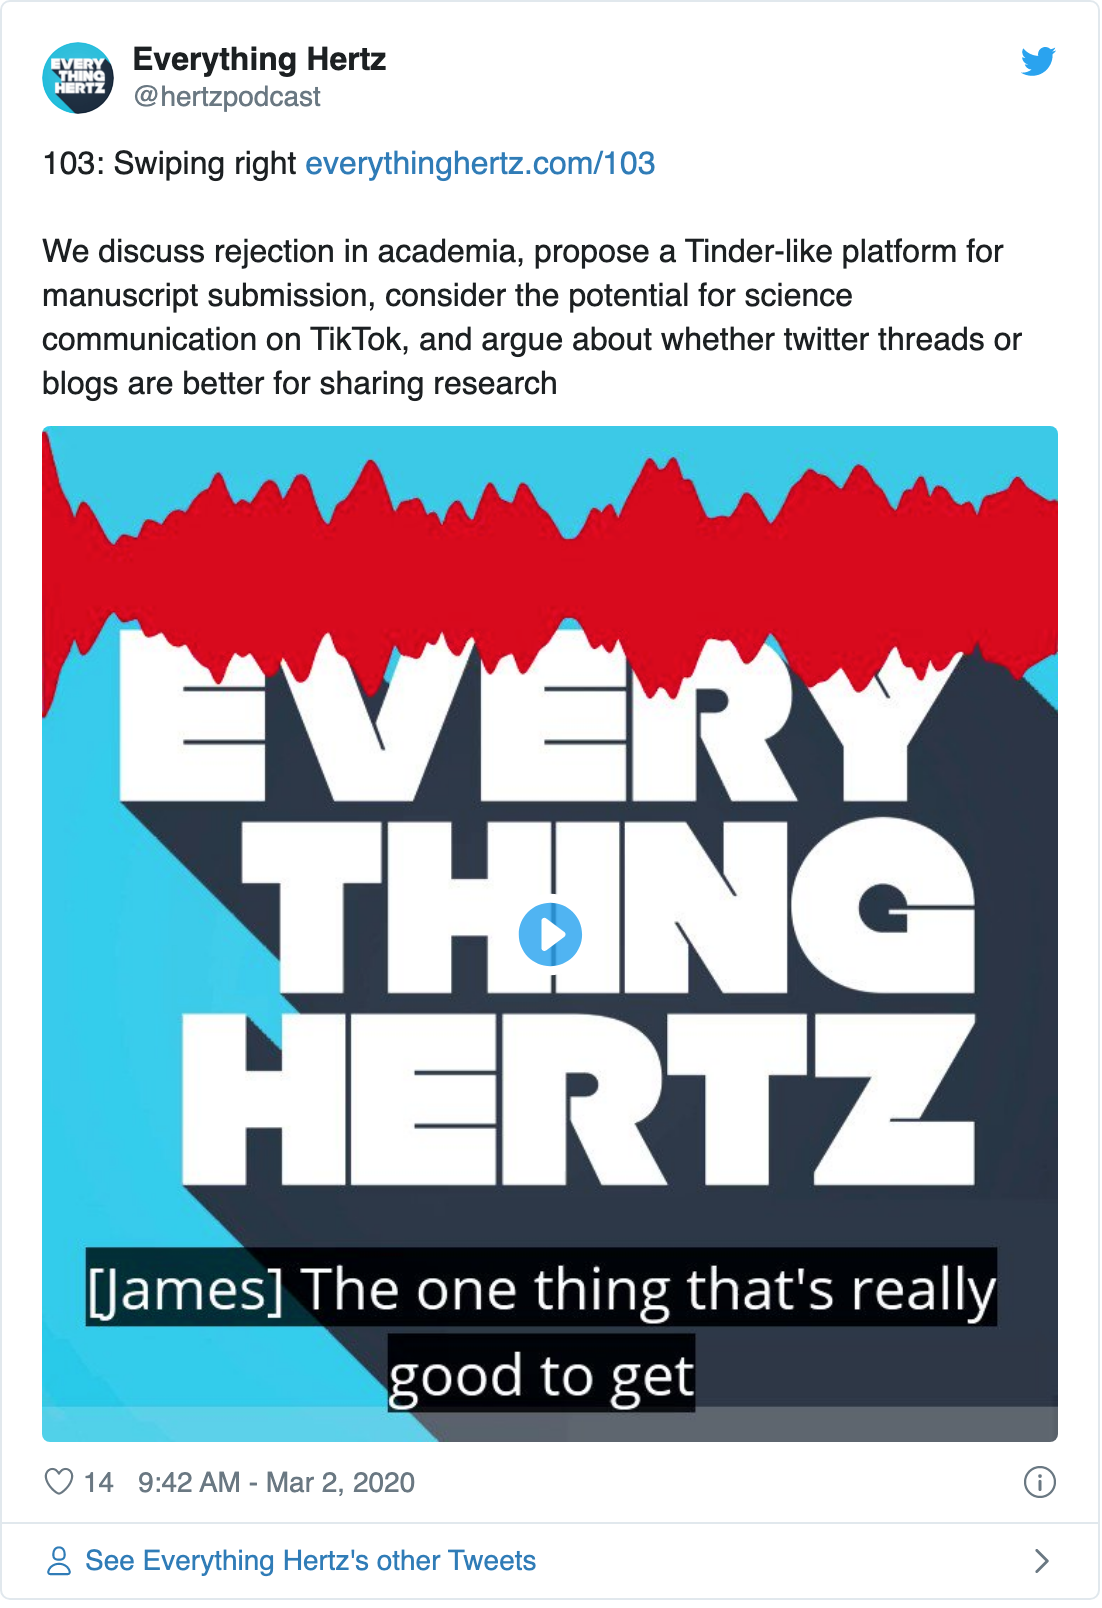
\includegraphics{twitter_book_files/figure-latex/tweet-audio-1.png}

Twitter doesn't automatically lend itself to sharing audio, but you can \href{https://www.dsquintana.blog/podcast-guide/}{create an audiogram and transribe the audio} (as the above clip) for easier sharing.

Twitter is also slowly rolling out an audio tweet feature.

\includegraphics{twitter_book_files/figure-latex/tweet-audio-feature-1.png}

As of writing, this feature is only available via the iOS Twitter app for limited accounts.

\hypertarget{care}{%
\chapter{Taking care of yourself on Twitter}\label{care}}

So far, I've covered all the benefits of Twitter. However, not everyone always has a positive experience on the platform. There are three main potential downsides to Twitter that I'm going to cover in this section.

\hypertarget{annoying-topics-or-users-clogging-your-feed}{%
\section*{Annoying topics (or users) clogging your feed}\label{annoying-topics-or-users-clogging-your-feed}}
\addcontentsline{toc}{section}{Annoying topics (or users) clogging your feed}

There might be some situations where people are tweeting a lot about a particular topic that you're not interested, such as when they're tweeting updates from a conference outside of your field. In these situations, you can mute specific users so they don't appear in your feed. They won't know that you've muted them and you're still following them. You can do this by clicking on the ``more'' button (the circle with three open circles) on a user's profile (Figure \ref{fig:mute}).

\begin{figure}

{\centering \includegraphics[width=0.8\linewidth]{images/mute} 

}

\caption{Muting a user}\label{fig:mute}
\end{figure}

You can also mute specific topics appearing in your timeline, for a set period of time (or forever) by adjusting your settings (Figure \ref{fig:mute-word}).

\begin{figure}

{\centering \includegraphics[width=0.8\linewidth]{images/mute_word} 

}

\caption{Muting a keyword}\label{fig:mute-word}
\end{figure}

\hypertarget{spending-too-much-time-on-twitter}{%
\section*{Spending too much time on Twitter}\label{spending-too-much-time-on-twitter}}
\addcontentsline{toc}{section}{Spending too much time on Twitter}

Twitter is designed to hold your attention for as long as possible, so it's no surprise that it can become addictive. The constant flow of new information and the intermittent reward of likes, retweets, and new followers makes it \emph{really easy} to get hooked. It wouldn't be this popular if it wasn't fun. This can become a problem, because if you're spending all your time on the platform then you'll have no work to share.

If you're like me, and you sometimes can't resist checking Twitter whenever you have a spare moment, there are desktop apps available, like \href{https://selfcontrolapp.com/}{\emph{SelfControl}} (MacOS) and \href{https://getcoldturkey.com/}{\emph{Cold Turkey}} (MacOS and Windows), which can block distracting websites. You may want to set this for smaller blocks or for entire days. Personally, I work in periods of forty minutes, in which I block all distracting websites. I take a 10-20 minute break between work sessions, and that's when I usually check Twitter.

It's fine if you want to take a break from the platform from time-to-time. As for me, I have occasional periods where I delete the Twitter app from my phone. I do this if I either have a very tight deadline or if I notice that I've been using the plafrom too much. The \href{https://support.apple.com/en-us/HT208982}{Screen Time} iOS app has been an eyeopener when it comes to my use. Don't let the reward of a couple more likes or followers overshadow lost hours of work.

\hypertarget{dealing-with-abusive-or-harmful-tweets}{%
\section*{Dealing with abusive or harmful tweets}\label{dealing-with-abusive-or-harmful-tweets}}
\addcontentsline{toc}{section}{Dealing with abusive or harmful tweets}

While not everyone has experienced harmful tweets, it is important to acknowledge that there have been some cases of harassment and verbal abuse in the Twitter science community. This will probably not be a regular experience for you, but it \emph{could} happen.

You can block accounts, which means they can't follow you or interact with you. Keep in mind that if they log out of their account which was blocked, they can see your tweets (if they're public). But they can no longer interact with you.

You can also report abusive or harmful tweets (or accounts) to Twitter, by following \href{https://help.twitter.com/en/safety-and-security/report-abusive-behavior}{these instructions}.

Ultimately, your wellbeing is more important than potentially getting a few extra followers and retweets. Don't be shy when it comes to blocking and muting people if required.

\hypertarget{one-month-twitter-bootcamp}{%
\chapter{One-month Twitter bootcamp}\label{one-month-twitter-bootcamp}}

If you're new to Twitter or you signed up in the past but haven't tweeted since, this one-month template will help get you started. For most days, I'll give you two options for what you can tweet.

This isn't a magic formula, simply a template for people to use who aren't sure how to get started with Twitter. Of course you can deviate from what I recommend here, but if you're not sure what to do, just refer to this guide.

As I've mentioned before, it's better to tweet too much than too little. When people look at your profile and decide whether to follow you, they're more likely to follow you if they see that you regularly tweet. This template provides a guide for what to tweet for twenty days, but bonus points if you also want to tweet on the weekends. I'll leave this up to you. Of course, you can do more than one tweet a day so this is just a minimum guideline.

\hypertarget{week-1}{%
\section*{Week 1}\label{week-1}}
\addcontentsline{toc}{section}{Week 1}

\hypertarget{day-1}{%
\subsection*{Day 1}\label{day-1}}
\addcontentsline{toc}{subsection}{Day 1}

Accountability is powerful, especially \emph{public} accountability, so your first tweet is going to announce your intention to tweet at least once every weekday for the first month. Here's an example: ``Over the next month I'm going to tweet at least once every weekday''.

Find about 50 people to follow (see section 1.6 for a refresher on finding people). As I mentioned in Chapter 1, don't follow too many people before you get started with this bootcamp.

\hypertarget{day-2}{%
\subsection*{Day 2}\label{day-2}}
\addcontentsline{toc}{subsection}{Day 2}

\begin{itemize}
\tightlist
\item
  Option 1: \protect\hyperlink{composing}{Share a study} that you've recently read. Remember to include an image (e.g., a screenshot of the abstract or a figure from the article) and tag the authors (if they're on Twitter). Just search their name + Twitter (e.g., ``Daniel Quintana twitter). If they have a more common name, try adding the term''scientist" or the field they're in (e.g., ``Chris Jackson geology twitter'').
\item
  Option 2: \protect\hyperlink{composing}{Share a summary} of one of your own studies, it doesn't have to be a recent one. If haven't published a paper yet, you can post a summary of your project plans.
\end{itemize}

\hypertarget{day-3}{%
\subsection*{Day 3}\label{day-3}}
\addcontentsline{toc}{subsection}{Day 3}

\begin{itemize}
\tightlist
\item
  Option 1: \protect\hyperlink{beginner}{Retweet} someone that you're following. Remember, if you find something interesting, there's a good chance your followers will find that interesting too
\item
  Option 2: Do a \protect\hyperlink{beginner}{quote-retweet}, in which you add a comment. This could be a simple as ``Here's an interesting paper''.
\end{itemize}

\hypertarget{day-4}{%
\subsection*{Day 4}\label{day-4}}
\addcontentsline{toc}{subsection}{Day 4}

\begin{itemize}
\tightlist
\item
  Option 1: Reply to someone's tweet with a comment. If you think that others would find this reply tweet useful, \protect\hyperlink{advanced}{retweet this tweet}.
\item
  Option 2: Ask a question using a \protect\hyperlink{intermediate}{hashtag} to target a specific community. For example, if you use the R statistical language, you use the \#Rstats hashtag. You can also ask general career questions using the \#PhDChat hashtag, if you're a graduate student.
\end{itemize}

\hypertarget{day-5}{%
\subsection*{Day 5}\label{day-5}}
\addcontentsline{toc}{subsection}{Day 5}

\begin{itemize}
\tightlist
\item
  Option 1: Share a tool that you use in your research (e.g., software)
\item
  Option 2: Post a link to a study that you've recently read
\end{itemize}

\hypertarget{week-2}{%
\section*{Week 2}\label{week-2}}
\addcontentsline{toc}{section}{Week 2}

\hypertarget{day-6}{%
\subsection*{Day 6}\label{day-6}}
\addcontentsline{toc}{subsection}{Day 6}

Now that you have a few tweets under your belt, follow another 50 people, or so.

\begin{itemize}
\item
  Option 1: Quote retweet something from one of the new people you just followed
\item
  Option 2: Reply to one of the tweets of the accounts you just followed
\end{itemize}

\hypertarget{day-7}{%
\subsection*{Day 7}\label{day-7}}
\addcontentsline{toc}{subsection}{Day 7}

\begin{itemize}
\tightlist
\item
  Option 1: Post the PowerPoint slides from one your presentations to Open Science Framework and share the link. Add the four best slides as images to your tweet. Don't forget to use images every opportunity you can. Alternatively, you can post a GIF preview of your entire slideshow:
\end{itemize}

\includegraphics{twitter_book_files/figure-latex/tweet-slideshow-1.png}

\begin{itemize}
\tightlist
\item
  Option 2: Share a paper you recently read and share the take-home message.
\end{itemize}

\hypertarget{day-8}{%
\subsection*{Day 8}\label{day-8}}
\addcontentsline{toc}{subsection}{Day 8}

\begin{itemize}
\tightlist
\item
  Option 1: Share a photo from your day (e.g., you lab, your desk, any books you're reading)
\item
  Option 2: Get meta and talk about how your finding this bootcamp
\end{itemize}

\hypertarget{day-9}{%
\subsection*{Day 9}\label{day-9}}
\addcontentsline{toc}{subsection}{Day 9}

\begin{itemize}
\tightlist
\item
  Option 1: Reply to a tweet
\item
  Option 2: Share a tool that you're currently using
\end{itemize}

\hypertarget{day-10}{%
\subsection*{Day 10}\label{day-10}}
\addcontentsline{toc}{subsection}{Day 10}

\begin{itemize}
\tightlist
\item
  Option 1: Post \protect\hyperlink{advanced}{a thread} describing one of your studies or your study plans (see section 4.1),
\item
  Option 1: \protect\hyperlink{intermediate}{Pin a new tweet} to your profile
\end{itemize}

\hypertarget{week-3}{%
\section*{Week 3}\label{week-3}}
\addcontentsline{toc}{section}{Week 3}

\hypertarget{day-11}{%
\subsection*{Day 11}\label{day-11}}
\addcontentsline{toc}{subsection}{Day 11}

Follow another 20 people, or so.

\begin{itemize}
\tightlist
\item
  Option 1: Ask a question using the \#ECRchat \protect\hyperlink{intermediate}{hashtag}
\item
  Option 2: Answer a question posed using the \#ECRchat \protect\hyperlink{intermediate}{hashtag}
\end{itemize}

\hypertarget{day-12}{%
\subsection*{Day 12}\label{day-12}}
\addcontentsline{toc}{subsection}{Day 12}

\begin{itemize}
\tightlist
\item
  Option 1: Post a link to music you're listening too (e.g., Spotify)
\item
  Option 2: Share the link to a paper that you've recently read and give a brief summary
\end{itemize}

\hypertarget{day-13}{%
\subsection*{Day 13}\label{day-13}}
\addcontentsline{toc}{subsection}{Day 13}

\begin{itemize}
\tightlist
\item
  Option 1: Post a \protect\hyperlink{intermediate}{Twitter poll}
\item
  Option 2: Share a link to software package or took you're currently using
\end{itemize}

\hypertarget{day-14}{%
\subsection*{Day 14}\label{day-14}}
\addcontentsline{toc}{subsection}{Day 14}

\begin{itemize}
\tightlist
\item
  Option 1: Make a video describing the results for one of your recent papers
\item
  Option 2: Comment on someone else's tweet
\end{itemize}

\hypertarget{day-15}{%
\subsection*{Day 15}\label{day-15}}
\addcontentsline{toc}{subsection}{Day 15}

\begin{itemize}
\tightlist
\item
  Option 1: Retweet someone
\item
  Option 2: Retweet someone and add a quote
\end{itemize}

\hypertarget{week-4}{%
\section*{Week 4}\label{week-4}}
\addcontentsline{toc}{section}{Week 4}

\hypertarget{day-16}{%
\subsection*{Day 16}\label{day-16}}
\addcontentsline{toc}{subsection}{Day 16}

Follow another 20 people, or so.

\begin{itemize}
\tightlist
\item
  Option 1: Post a picture of your work in progress (e.g., a manuscript draft, a scientific figure, programming code)
\item
  Option 2: Post a picture of your hobby
\end{itemize}

\hypertarget{day-17}{%
\subsection*{Day 17}\label{day-17}}
\addcontentsline{toc}{subsection}{Day 17}

\begin{itemize}
\tightlist
\item
  Option 1: Post a link to a study that you've recently read
\item
  Option 2: Share a summary of one of your own studies or your project plans.
\end{itemize}

\hypertarget{day-18}{%
\subsection*{Day 18}\label{day-18}}
\addcontentsline{toc}{subsection}{Day 18}

\begin{itemize}
\tightlist
\item
  Option 1: Share a \protect\hyperlink{composing}{meme}
\item
  Option 2: Share a link to a book your reading (or a podcast you're listening to)
\end{itemize}

\hypertarget{day-19}{%
\subsection*{Day 19}\label{day-19}}
\addcontentsline{toc}{subsection}{Day 19}

\begin{itemize}
\tightlist
\item
  Option 1: Answer a question asked using the \#ECRchat (or similar) hashtag
\item
  Option 2: Ask a question asked using the \#ECRchat (or similar) hashtag
\end{itemize}

\hypertarget{day-20}{%
\subsection*{Day 20}\label{day-20}}
\addcontentsline{toc}{subsection}{Day 20}

\begin{itemize}
\tightlist
\item
  Tweet that you've completed your one-month Twitter bootcamp
\end{itemize}

\hypertarget{acknowledgements}{%
\chapter{Acknowledgements}\label{acknowledgements}}

Thanks to \href{https://twitter.com/_DaniBeck}{@\_DaniBeck}, \href{https://twitter.com/PsyBrief}{@PsyBrief}, \href{https://twitter.com/@ChelseaParlett}{@ChelseaParlett}, \href{https://twitter.com/BrianPulling}{@BrianPulling},
\href{https://twitter.com/dhlwilson}{@dhlwilson}, and \href{https://twitter.com/biomechstu}{@biomechstu} who provided feedback on a draft version of this book.

The lightglobe icon was created by \href{https://twitter.com/dcossyle}{@dcossyle} and downloaded from \href{https://desiree.rbind.io/post/2019/making-tip-boxes-with-bookdown-and-rmarkdown/}{this page}. The salt shaker icon was made by \href{https://www.flaticon.com/authors/freepik}{Freepik} from \href{http://www.flaticon.com/}{www.flaticon.com}.

Thanks to \href{https://twitter.com/grrrck}{@grrrck} for his work on the \href{https://github.com/gadenbuie/tweetrmd}{`tweetmd' R package}.

I wrote and published this book using the \href{https://bookdown.org/}{bookdown R package} and host the book on \href{https://github.com/dsquintana/t4scientists}{Github}. I first learned about these tools on Twitter, of course.

  \bibliography{book.bib,packages.bib}

\end{document}
